\documentclass[12pt]{report}

% Paquetes LaTeX y estilos globales
\usepackage[utf8]{inputenc}
\usepackage{multicol}
\usepackage{xcolor}
\usepackage{subfigure}
\usepackage[english]{babel}
\usepackage[utf8]{inputenc}
\usepackage{graphicx}
\usepackage{titlesec}
\usepackage[bookmarks,breaklinks,colorlinks=true,allcolors=blue]{hyperref}
\usepackage{listings}
\usepackage{inconsolata}
\usepackage{float}
\usepackage{mathpazo} % Fuente Palatino
\usepackage[labelfont=bf]{caption}
\usepackage{multirow}

\usepackage[square,numbers]{natbib}
\usepackage[nottoc,notlof,notlot]{tocbibind}  % Mete la bibliografía como capítulo en la TOC, los parámetros excluyen los otros índices de aparecer también
\usepackage{geometry}
\usepackage{amsmath}
\usepackage{parskip}
\usepackage[official]{eurosym}
\usepackage{todonotes}
\usepackage{csquotes}
\usepackage{tocbasic}  % Estilos de la TOC
% Formato del título de capítulos y secciones
\titleformat{\chapter}[block]{\normalfont\huge\bfseries}{\thechapter.}{.5em}{\Huge}[\vspace{2pt}{\titlerule[2pt]}]

\titlespacing*{\chapter}{0pt}{-19pt}{25pt}

\titleformat{\section}[block]{\normalfont\Large\bfseries}{\thesection.}{.5em}{\Large}

\titleformat{\part}[block]{\titlerule[2pt]\normalfont\Huge\bfseries\centering}{Parte \Roman{part}\\\vspace{15pt}}{0pt}{\Huge}[\vspace{2pt}{\titlerule[2pt]}]

% Tamaños y estilos de elementos en la TOC
\DeclareTOCStyleEntry[
    linefill=\bfseries\TOCLineLeaderFill,
    beforeskip=12pt,
    entrynumberformat=\chapterprefixintoc,
    entryformat=\chaptertocformat,
    pagenumberformat=\chaptertocformat,
    dynnumwidth
]{tocline}{chapter}

\DeclareTOCStyleEntry[
    % linefill=\bfseries\TOCLineLeaderFill,
    beforeskip=30pt,
    entrynumberformat=\chapterprefixintoc,
    entryformat=\parttocformat,
    pagenumberformat=\partpagetocformat,
    numwidth=0pt
]{tocline}{part}

\newcommand\chaptertocformat[1]{\large{\textbf{#1}}}%
\newcommand\chapterprefixintoc[1]{#1}%
\newcommand\parttocformat[1]{\Large{\textbf{#1}}}%
\newcommand\partpagetocformat[1]{} % Don't print the page number for parts

% Alias para estilos de texto comunes
\newcommand{\negritas}[1]{\textbf{#1}}
\newcommand{\cursiva}[1]{\textit{#1}}
\newcommand{\codigo}[1]{\texttt{#1}}

% Formato del código fuente con lstlisting
\lstset{
  basicstyle=\ttfamily,
  breaklines=true,
}

% Márgenes
\geometry{
    a4paper,
    margin=2.75cm
}
\setlength{\marginparwidth}{2cm} 

% Limite de profundidad del índice
\setcounter{tocdepth}{2}

% Eliminar el guionado
\tolerance=1
\emergencystretch=\maxdimen
\hyphenpenalty=10000
\hbadness=10000

% Indentación de párrafos
\setlength{\parindent}{.75cm}

\renewcommand{\lstlistingname}{Code extract}
\renewcommand*{\lstlistlistingname}{Code excerpt indexcode excerpt}

% Comandos para establecer variables
\newcommand{\setTitle}[1]{\def\tfgTitle {#1}}
\newcommand{\setAuthor}[1]{\def\tfgAuthors {#1}}
\newcommand{\setDegree}[1]{\def\tfgDegree {#1}}
\newcommand{\setSupervisor}[1]{\def\tfgSupervisor {#1}}
\newcommand{\setDepartment}[1]{\def\tfgDepartment {#1}}
\newcommand{\setMonth}[1]{\def\tfgMonth {#1}}
\newcommand{\setYear}[1]{\def\tfgYear {#1}}
\newcommand{\setDedication}[1]{\def\tfgDedication {#1}}

% Estilos para el código
% Configuración genérica
\definecolor{codegreen}{rgb}{0,0.6,0}
\definecolor{codegray}{rgb}{0.5,0.5,0.5}
\definecolor{codepurple}{rgb}{0.58,0,0.82}
\definecolor{editorOcher}{rgb}{0.8, 0.3, 0} % #FF7F00 -> rgb(239, 169, 0)
\definecolor{editorGreen}{rgb}{0, 0.5, 0} % #007C00 -> rgb(0, 124, 0)

\lstdefinestyle{listingstyle}{
    backgroundcolor=\color{white},  
    keywordstyle=\bfseries\color{blue},
    numberstyle=\tiny\color{codegray},
    stringstyle=\color{editorGreen},
    commentstyle=\color{codegray},
    basicstyle=\ttfamily\color{black},
    breakatwhitespace=false,         
    breaklines=true,                 
    captionpos=b,                    
    keepspaces=true,                 
    numbers=left,                    
    numbersep=5pt,                  
    showspaces=false,                
    showstringspaces=false,
    showtabs=false,                  
    tabsize=2,
    frame=tb,
    keywords=[2]{True,False},
    literate=%
*{0}{{{\color{editorOcher}0}}}1
{1}{{{\color{editorOcher}1}}}1
{2}{{{\color{editorOcher}2}}}1
{3}{{{\color{editorOcher}3}}}1
{4}{{{\color{editorOcher}4}}}1
{5}{{{\color{editorOcher}5}}}1
{6}{{{\color{editorOcher}6}}}1
{7}{{{\color{editorOcher}7}}}1
{8}{{{\color{editorOcher}8}}}1
{9}{{{\color{editorOcher}9}}}1,
}

\lstset{style=listingstyle}
\lstset{columns=fullflexible}

\lstdefinelanguage{css}{
  keywords={color,background-image:,margin,padding,font,weight,display,position,top,left,right,bottom,list,style,border,size,white,space,min,width, transition:, transform:, transition-property, transition-duration, transition-timing-function},	
  sensitive=true,
  morecomment=[l]{//},
  morecomment=[s]{/*}{*/},
  morestring=[b]',
  morestring=[b]",
  alsoletter={:},
  alsodigit={-}
}
% JavaScript
\lstdefinelanguage{javascript}{
  morekeywords={abstract, arguments, await, boolean, break, byte, case, catch, char, class, const, continue, debugger, default, delete, do, double, else, enum, eval, export, extends, false, final, finally, float, for, function, goto, if, implements, import, in, instanceof, int, interface, let, long, native, new, null, package, private, protected, public, return, short, static, super, switch, synchronized, this, throw, throws, transient, true, try, typeof, var, void, volatile, while, with, yield},
  morecomment=[s]{/*}{*/},
  morecomment=[l]//,
  morestring=[b]",
  morestring=[b]'
}


%%%%%%%%%%%%%%%%%%%%%%%%%%%%%%%%%%%%%%%%%%%%%%%%%%%%%%%%%%%%%%%%%%%%%%%%%%%%%%%%%%%%%

% Variables para la portada
\setTitle{Reconocimiento de relaciones del genoma con la respuesta ante el cáncer}
\setAuthor{Sergio Santiago Sánchez} % Si hay más de un autor, separarlos con \\
\setDegree{Master's Degree in Logic, Computation and Artificial Intelligence} % Cambiar si es necesario
\setSupervisor{Miguel Ángel Gutiérrez Naranjo \\Miguel Cárdenas Montes} % Si hay más de un tutor, separarlos con \\
\setMonth{July } % Dejar sólo el mes de la convocatoria en que se presenta el trabajo
\setYear{2024/25} % Por ejemplo, 2022/23

%%%%%%%%%%%%%%%%%%%%%%%%%%%%%%%%%%%%%%%%%%%%%%%%%%%%%%%%%%%%%%%%%%%%%%%%%%%%%%%%%%%%%

% Dedicatoria del trabajo
% Si no se desea incluir, comentar o borrar la línea siguiente para eliminar la página de dedicatoria
\setDedication{Aquí la dedicatoria del trabajo}

%%%%%%%%%%%%%%%%%%%%%%%%%%%%%%%%%%%%%%%%%%%%%%%%%%%%%%%%%%%%%%%%%%%%%%%%%%%%%%%%%%%%%

% Comienzo del documento
\begin{document}

    % Portada y secciones no numeradas
    \thispagestyle{empty} % Impide que se incluya número de página en la portada
\begin{center}

\vspace*{1cm}


\includegraphics[width=\textwidth]{figures/etsii_us.png}

\vspace*{3cm}
\begin{large}
MASTER'S THESIS
\end{large}

\vspace*{0.1in}
\textbf{\huge \tfgTitle}

\vspace*{.2in}

{\large Written by}\\
\textbf{\Large \tfgAuthors}

\vspace*{3cm}

\textbf{To obtain the title of}\\
{\large \tfgDegree}

\vspace*{0.2in}

\textbf{Advisors}\\
{\large \tfgSupervisor}\\

\vspace*{0.2in}


\vspace*{.6in}
\textbf{\Large \tfgMonth  Examination Session, Curse \tfgYear}

\end{center}

% Dedicatoria
\ifdefined\tfgDedication
    \newpage
    \thispagestyle{empty}
    
    \vspace*{\fill}
    \begin{center}
    \textit{\tfgDedication}
    \end{center}
    \vspace*{\fill}
\fi

\clearpage\setcounter{page}{1} % Comienza a incluir números de página a partir de aquí
\pagenumbering{roman} % En números romanos
    \chapter*{Acknowledgments}

I would like to thank all my friends who have supported me, both by helping me to disconnect and by motivating me during the most difficult moments of my research. But I would particularly like to highlight the help of Nicole, who has encouraged me to keep going at all times, cheered me up when I needed it and spent many hours reviewing what caused me the most uncertainty: writing in English. Without your help, I probably wouldn't have finished on time.

I would also like to express my gratitude to my two tutors, Miguel Cárdenas and Miguel Ángel Gutiérrez, for their patience throughout the development of this work. I sincerely appreciate their willingness to correct my mistakes, as well as their efforts to find time to meet with me and guide me, even in difficult moments.
    \chapter*{Resumen}
Incluya aquí un resumen de los aspectos generales de su trabajo, en español.

\vspace{.5cm}

\textbf{Palabras clave:} Palabra clave 1, palabra clave 2, ..., palabra clave N
    \chapter*{Abstract}
Genetically personalised therapies for treating cancer are showing great advances, improving patients' quality of life and life expectancy. However, there is a key challenge in this type of treatment, as it is currently impossible to accurately predict a person's response to a drug, which is a major problem. If the treatment is too intense, not only will it not help the patient, but it will also worsen their condition.

This study makes use of the Genomics of Drug Sensitivity in Cancer (GDSC) dataset, which includes information on genomic and pharmacological profiles and data on the characteristics of cancer cell lines, constituting a great source of information. To exploit this data, algorithms based on both neural networks and trees have been used, always with the aim of providing a model that is not only accurate but also useful to society.

The research aims to obtain a model capable of predicting the  \(LN\_IC_{50}\) variable, which is an indicator of the concentration of drug needed to inhibit the growth of cancer cells by 50%.

The resulting model has, in turn, been validated using explainability techniques, providing certainty about the reliability of the predictions and demonstrating that genetic profiles influence the patient's response to cancer drugs.

\vspace{.5cm}

\textbf{Keywords:} cancer, drug response, treatment effectiveness, neural networks, XGBoost, explainability, SHAP.
    
    % Índice del documento y de figuras
    \begingroup
        % Los enlaces son normalmente azules, pero en los índices se configuran a negro para que no aparezca todo azul
        \hypersetup{linkcolor=black}
        \tableofcontents
        \listoffigures
        \listoftables
        \lstlistoflistings
    \endgroup
    
    % Cambia el estilo de números de página de romanos a normal
    \clearpage\pagenumbering{arabic}
    
    % Capítulos del trabajo
    %\chapter{Ejemplos de uso de LaTeX}\label{cap:ejemplos}

\todo[inline]{Este capítulo se incluye únicamente como ayuda y referencia de uso de \LaTeX. No debe aparecer en el documento final.}

\section{Introducción}
En este capítulo se muestran ejemplos de uso de \LaTeX{} para operaciones comunes. 

\section{Estilos}\label{sec:estilos}
Se pueden aplicar estilos al texto como \textbf{negritas}, \textit{cursiva}, \underline{subrayado} y \texttt{monoespaciado}. También se \textcolor{red}{pueden} \textcolor{blue}{aplicar} \textcolor{green}{colores}, y \underline{\textit{combinar}} \textbf{\textcolor{red}{estilos}}. Se recomienda usar sólo negritas para hacer énfasis, y no abusar de este recurso.

Por comodidad para usuarios no habituados con LaTeX, esta plantilla define algunos alias de comandos más fáciles de recordar para estilos de texto comunes: \negritas{negritas}, \cursiva{cursiva} y \codigo{código}.

\section{Listados}
Con itemize se pueden crear listas no numeradas:

\begin{itemize}
    \item Fresas
    \item Melocotones
    \item Piñas
    \item Nectarinas
\end{itemize}

De manera similar, enumerate permite crear listas numeradas:

\begin{enumerate}
    \item Elaborar la memoria del TFG
    \item Elaborar la presentación
    \item Presentar el TFG
    \item Solicitar el título de Grado
\end{enumerate}

\section{Subsecciones}
Se pueden definir subsecciones con el comando \texttt{subsection}:

\subsection{Primera subsección}\label{sec:subseccion}
Esto es una subsección

\subsection{Segunda subsección}
Esto es otra subsección.

\subsubsection{Sub-sub-sección}
Este es un tercer nivel de profundidad, que no aparece en el índice general. Se recomienda no utilizarlo, si es posible.

\section{Imágenes y figuras}
Todas las imágenes y figuras del documento se incluirán en la carpeta ``figures''. Se pueden incluir de la siguiente manera:

\begin{figure}[htp]
    \centering
    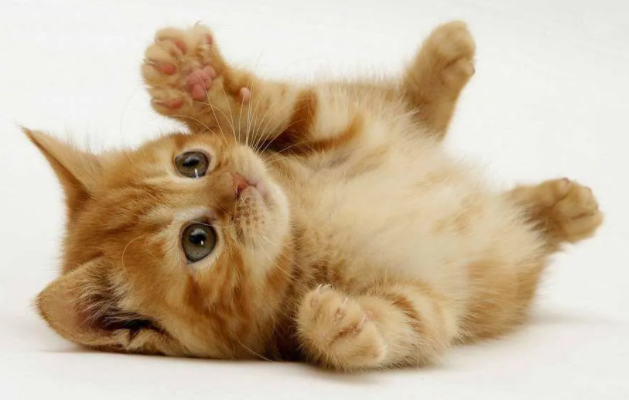
\includegraphics[width=0.7\textwidth]{figures/ejemplo.png}
    \caption{Un feroz depredador}
    \label{fig:ejemplo}
\end{figure}

Observe que las figuras se numeran automáticamente según el capítulo y el número de figuras que hayan aparecido anteriormente en dicho capítulo. Existen muchas maneras de definir el tamaño de una figura, pero se aconseja utilizar la mostrada en este ejemplo: se define el ancho de la figura como un porcentaje del ancho total de la página, y la altura se escala automáticamente. De esta manera, el ancho máximo de una figura sería 1.0 * textwidth, lo que aseguraría que se muestra al máximo tamaño posible sin sobrepasar los márgenes del documento.

Tenga en cuenta que LaTeX intenta incluir las figuras en el mismo sitio donde se declaran, pero en ocasiones no es posible por motivos de espacio. En esos casos, LaTeX colocará la figura lo más cerca posible de su declaración, puede que en una página diferente. Esto es un comportamiento normal.

\section{Tablas}
Existe una gran variedad de formas de crear tablas en LaTeX puro, y todas ellas tienen cierta complejidad. A continuación se muestra un ejemplo simple de tabla nativa, en la Tabla \ref{table:ejemplo}. Se recomienda crear un archivo en la carpeta \textit{tables} por cada tabla nativa que se desee incluir, y enlazarla mediante el comando \texttt{input}.

\begin{table}[htp]
\centering

    % Esta primera línea define las columnas de la tabla. Los posibles tipos de columna son:
    % c: texto centrado
    % l: texto alineado a la izquierda
    % r: texto centrado a la derecha
    % p: columna de ancho fijo
    % Las columnas tienen ancho dinámico según la anchura máxima de los elementos que contengan.

    % Las columnas l/r/c no parten el texto en filas diferentes si éste es demasiado largo. Para ello, puede utilizar el tipo de columna de ancho fijo "p".
    
    % Las barras verticales | se usan para definir los bordes verticales de la tabla. Pruebe a eliminar algunas y observe qué ocurre.
    \begin{tabular}{ | l | c | r | p{2cm} | }
        
        % A continuación van las filas de la tabla. En cada fila, las columnas se separan con el carácter &
        % Para terminar una fila se usa \\
        % Para incluir un borde horizontal entre filas se usa \hline

        % Cabecera con textos en negrita:
        \hline
        \textbf{Columna L} & \textbf{Columna C} & \textbf{Columna R} & \textbf{Columna P}\\
        \hline
        
        % Cuerpo de la tabla:
        Texto de ejemplo & Texto de ejemplo & Texto de ejemplo & Texto de ejemplo\\
        \hline
        ABC & DEF & HIJ & KLM\\
        \hline
        
    \end{tabular} 
    
    \caption{Tabla LaTeX de ejemplo}
    \label{table:ejemplo} 
\end{table}


Para tablas con un formato más complejo, considere la posibilidad de diseñarla usando otro software externo (por ejemplo Excel) e incluirla de manera similar a una figura. \textbf{Observe en el código LaTeX a continuación cómo usar el comando \texttt{captionof\{table\}}, en lugar de simplemente \texttt{caption}, hace que se liste como una Tabla en lugar de como una Figura}:

\begin{figure}[htp]
    \centering
    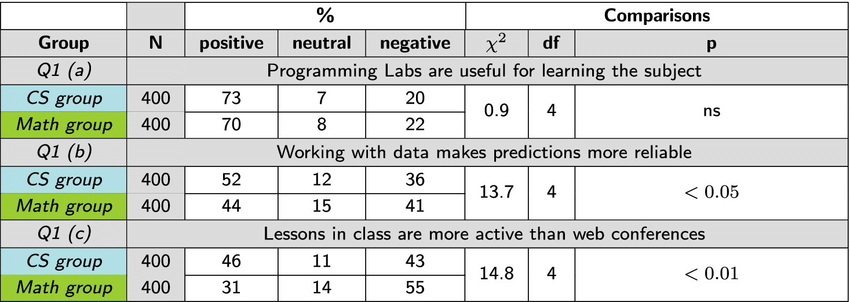
\includegraphics[width=1.0\textwidth]{tables/complex_table.png}
    \captionof{table}{Tabla compleja introducida como figura}
    \label{table:ejemplo2}
\end{figure}

\section{Referencias}
Observe cómo en el código fuente de esta sección se ha usado varias veces el comando \texttt{label}. Este comando permite marcar un elemento, ya sea capítulo, sección, figura, etc. para hacer una referencia numérica al mismo. Para referenciar una label se usa el comando \texttt{ref} incluyendo el nombre de la referencia:

Este es el capítulo \ref{cap:ejemplos}.

En la sección \ref{sec:estilos} se muestran ejemplos de estilos.

La subsección \ref{sec:subseccion} explica...

En la Figura \ref{fig:ejemplo} vemos que...

Esto evita que tengamos que escribir directamente los índices de las secciones y figuras que queremos mencionar, ya que LaTeX lo hace por nosotros y además se encarga de mantenerlos actualizados en caso de que cambien (pruebe a mover este capítulo al final del documento y observe cómo se actualizan automáticamente todos los índices referenciados). Además, las referencias mediante ``ref'' actúan como hipervínculos dentro del documento que llevan al elemento referenciado al pulsar en ellas.

Es habitual nombrar las ``label'' con un prefijo que indica el tipo de elemento para encontrarlo luego más fácilmente, pero no es obligatorio.

\section{Extractos de código}

Se pueden incluir extractos de código mediante lstlisting:

\begin{lstlisting}[language=Python, caption={Código Python}, label={cod:python}, captionpos=b]
num = float(input("Enter a number: "))
if num > 0:
   print("Positive number")
elif num == 0:
   print("Zero")
else:
   print("Negative number")
\end{lstlisting}

Para evitar tener que incluir el código directamente en el texto del documento, se pueden guardar en archivos separados y referenciarlos:

\lstinputlisting[
    float,
    floatplacement=!htp,
    language=Java,
    label=cod:java,
    caption=Código Java
]{code/java_example.java}

\lstinputlisting[
    float,
    floatplacement=!htp,
    language=html,
    label=cod:html,
    caption=Código HTML
]{code/html_example.html}

\lstinputlisting[
    float,
    floatplacement=!htp,
    language=javascript,
    label=cod:js,
    caption=Código JavaScript
]{code/javascript_example.js}

Los extractos de código también se pueden referenciar mediante label/ref: Extractos de código \ref{cod:python}, \ref{cod:java}, \ref{cod:html}, \ref{cod:js}. 

\section{Enlaces}
Puede enlazar una web externa mediante el comando \texttt{url}: \url{https://www.example.com}. También se puede vincular un enlace a un texto mediante el comando href: \href{https://www.example.com}{dominio de ejemplo}.

\section{Citas y bibliografía}
En LaTeX, los elementos de la bibliografía se almacenan en un fichero bibliográfico en un formato llamado BibTeX, en el caso de este proyecto se encuentran en ``bibliografia.bib''. Para citar un elemento se usa el comando \texttt{cite}. Se pueden citar tanto artículos científicos \cite{borrego2019} como enlaces web \cite{webETSII}. 

También se puede usar el comando \texttt{citet} para incluir una referencia junto con el nombre de su autor o autores: \citet{borrego2021}. Todas las citas se numeran automáticamente y se incluyen en la sección de bibliografía del trabajo. El orden por defecto es según su orden de aparición en el documento. Para ordenarlas por orden alfabético del autor, puede modificar el comando \texttt{bibliographystyle} del archivo principal y reemplazar su valor por el estilo \texttt{plainnat} (orden alfabético, nombres completos) o \texttt{abbrvnat} (orden alfabético, nombres abreviados).

Observe cómo los elementos bibliográficos almacenados en ``bibliografia.bib'' tienen una etiqueta asociada, que es la que se usa al citarlos mediante cite. \textbf{Añadir una referencia al fichero bibliográfico no hace que ésta aparezca automáticamente en la sección de bibliografía del trabajo, es necesario citarla en algún lugar del mismo}.

\section{Ecuaciones}
LaTeX tiene un potente motor para mostrar ecuaciones matemáticas y un amplio catálogo de símbolos matemáticos. El entorno matemático se puede activar de muchas maneras. Para incluir ecuaciones simples en un texto se pueden rodear de símbolos dólar: $1 + 2 = 3$, $\sqrt{81} = 3^2 = 9$, $\forall x \in y~\exists~z : S_z < 4$.

Las ecuaciones más complejas pueden expresarse aparte y son numeradas: ecuación \ref{eq:ecuacion}.

\begin{equation}\label{eq:ecuacion}
\lim_{x\to 0}{\frac{e^x-1}{2x}}
 \overset{\left[\frac{0}{0}\right]}{\underset{\mathrm{H}}{=}}
 \lim_{x\to 0}{\frac{e^x}{2}}={\frac{1}{2}}
 +7 \int_0^2
  \left(
    -\frac{1}{4}\left(e^{-4t_1}+e^{4t_1-8}\right)
  \right)\,dt_1
\end{equation}

Dispone \href{http://www.yann-ollivier.org/latex/texsymbols.pdf}{aquí} de un amplio listado de símbolos que pueden usarse en modo matemático.

\section{Caracteres y símbolos especiales}
Algunos caracteres y símbolos deben ser escapados para poder representarse en el documento, ya que tienen un significado especial en LaTeX. Algunos de ellos son:

\begin{itemize}
    \item El símbolo dólar \$ se usa para ecuaciones.
    \item El tanto por ciento \% se usa para comentarios en el código fuente.
    \item El símbolo euro \euro{} suele dar problemas si se escribe directamente.
    \item El guión bajo \_ se usa para subíndices en modo matemático.
    \item Las comillas deben expresarse `así' para comillas simples y ``así'' para comillas dobles. Las comillas españolas pueden expresarse \textquote{así}.
    \item La barra invertida o contrabarra \textbackslash{} se usa para comandos LaTeX.
    \item Otros símbolos que deben escaparse son las llaves \{ \}, el ampersand \&, la almohadilla \# y los símbolos mayor que \textgreater{} y menor que \textless{}.
\end{itemize}
    \chapter{Introduction and motivations}\label{cap:introduccion}

There is currently an extensive body of publicly available research foccused on finding a cure for cancer. The open access \cite{tcga_nci} \cite{gdsc_website} to much of this work enables researchers worldwide to build on it working with the community. This is how the scientific community tries to continue the chain until it achieves findings that can save lives. 

One line of research is the effect of a drug based on the patient's genome. There are records of patients and studies with the same medication and type of cancer but with different responses to treatment \cite{genomicBiology} \cite{metastasisCancer}. This variability raises critical questions, especially regarding the personalization of therapy. Decisions about which medication to administer and in what dosage directly affect people's quality of life. If a patient receives an excessive amount of medication, the consequences can be even worse than those of the cancer itself. Similarly, if the amount administered is less than required, the effects will not be as desired.

One of the main challenges of applying machine learning techniques to this type of research lies in the very nature of the data, which poses significant limitations. Generally, it is highly variable, with cancer records showing a large number of treatments for the same type, and often containing a considerable amount of noise or missing values. At the same time, genetic information is very extensive, further complicating the search for a model that meets all requirements.

To address these challenges, the proposed models must be highly robust in the face of different datasets. They must be able to function correctly despite noise and missing values.  In addition, these models must be updated regularly so that new knowledge about the disease is always available to provide quality predictions. Without these periodic predictions, the risk of obsolescence increases dangerously.

This is undoubtedly one of the most demanding and sensitive areas of research, not only due to its technical complexity, but also because of the profound human responsibility it entails. Working with data derived from serious illnesses such as cancer requires a constant awareness that behind each data point is a person, with their own story, struggle, and hope. The outcomes of such research have the potential to significantly improve patient care and quality of life. However, this potential is accompanied by a high degree of responsibility: a robust and well-validated finding can guide more effective treatments, while an error or oversight could lead to inappropriate clinical decisions, potentially harming lives. In this sense, the stakes are exceptionally high. It is a field that demands not only technical excellence but also ethical rigor, caution, and empathy. The risks are substantial but so are the opportunities to make meaningful, life-changing contributions to human health.
    \chapter{Core Knowledge}\label{cap:planificación}

\section{Introduction}

There are currently numerous techniques used in artificial intelligence. These not only come from physics or mathematics, but are also closely related to economics and computer science. Such is the catalog of possibilities available to us that it is often difficult to keep up to date, as new ideas emerge every day. Therefore, in order to obtain a better general understanding of this work, we will explain the principles of some of the methods or techniques used in the project, since understanding them will make it easier to follow the workflow. 
s
\section{Neural Networks}

If we look at the history of science and technology, we can observe that many advances are inspired by real biological systems. For example, a camera shares many similarities with the human eye. Another example is the processor, which consists of a large number of transistors connected to perform calculations. Neural networks are also part of this trend, as their structure is approximately based on biological neural networks. 

Neural networks are a type of machine learning model inspired by the human brain. They are designed to recognise patterns or relationships between data. This feature makes them the ideal type of model for images, language processing, or predictive modelling.

To fully comprehend this research, it is necessary to understand the following concepts.

\subsection{Relevant layers for this research}

There are numerous options available when selecting the appropriate layers for a neural network, each serving a distinct and well-defined purpose. Given the wide variability of existing architectures, this study will briefly describe the most influential layer types employed during the research, focusing on those that had the most significant impact on model performance and learning behavior.

\begin{itemize}
    \item \textbf{Dense}: Also known as fully connected, it is one of the simplest and best-known layers. Each neuron receives one input from each neuron in the previous layer and produces one output per neuron.
    \item \textbf{Convolutional 1D layers}: This is a layer used in neural networks to process sequential information, such as text, audio or genes. It allows one-dimensional convolution filters to be applied, thereby extracting relationships and patterns from the data. The output of a Conv1D layer is a feature map that captures the patterns extracted from the input data. These maps highlight local relationships in the sequence, such as recurring motifs or trends. However, one potential drawback of stacking many convolutional layers is that the original low-level information can become increasingly abstract or diluted. While deeper layers tend to capture more complex features, they may also lose fine-grained details present in the raw data.
\end{itemize}

\subsection{Regularization methods}

Regularisation is applied to machine learning models to prevent overfitting, which occurs when they learn the training data too well, including noise and outliers. This results in poorer generalisation when faced with new data.

Some examples include:
\begin{itemize}
    \item \textbf{L1 and L2 regularization}: Also known as Lasso (L1) and Ridge (L2) regularization, these techniques help prevent the model's weights from becoming too large. L1 Regularization encourages sparsity by driving less relevant weights to zero, effectively performing feature selection. L2 Regularization penalizes large weights more smoothly, distributing the error and promoting generalization.
    \item \textbf{Dropout}: This layer allows some neurons to be randomly reset to zero. This prevents the network from becoming overly dependent on a single neuron, thus avoiding overfitting.
    \item \textbf{Spatial dropout 1D}: This is an adaptation of dropout to networks in which convolutional layers are applied, so that the dimension of spatial dropout depends on the dimension of the convolutional layer, in this case 1.
    \item \textbf{Batch normalization}: Used to standardise the input to the layers, it reduces the impact of weight initialisation. It is very important to apply this layer before the activation function and not afterwards.
    \item \textbf{Max pooling}: It allows you to reduce the dimensionality of feature maps by selecting the maximum available using a sliding window.
\end{itemize}



\section{Predictions trees}

Decision trees are one of the most widely used types of machine learning algorithms, due not only to their great predictive power but also to their ease of interpretation, both in classification and regression tasks. The idea behind this algorithm is to divide the dataset into increasingly smaller subsets.

One of the main advantages is the interpretability they offer, without the need for any type of complex preprocessing or scaling. This makes them widely used in domains where understanding the reason behind each decision is important, such as biology or chemistry.

However, they do have disadvantages. For example, they are prone to overfitting, although there are techniques such as a posteriori pruning, maximum depth or minimum number of examples per leaf, to avoid this. But undoubtedly, the main drawback is that they are unable to generalise correctly when the test data falls outside the training domain.

The main types of tree algorithms include:

\begin{itemize}
    \item \textbf{CART}: It is a foundational decision tree algorithm, used for regression or classification tasks. It uses the Gini index or MSE to divide the data into different subsets, depending on whether it is a classification or regression problem.
    \item \textbf{RandomForest}: It is an ensemble learning method \footnote{Algorithms that combine several models, usually of the same type, produce an output based on all of them, applying techniques such as average voting.} used for both classification and regression tasks. It builds upon decision trees by combining multiple trees, which are independent, and aggregating their results to improve accuracy and reduce overfitting.
    \item \textbf{Gradient Boosted Trees}: This technique combines different decision trees, but unlike RandomForest, they are not independent. Each tree is trained with the aim of improving on those examples where the previous one failed. An example of this type of algorithm is XGBoost.
\end{itemize}

\section{SHAP values}

Based on Shapley values from cooperative game theory, SHAP is capable of measuring the contribution of a feature to a result, i.e., it quantifies the contribution of variables to the model output, both locally, a single example, and globally, the entire dataset. This allows us to determine which variables are most relevant in a prediction. 

The main advantage of SHAP over other explainability algorithms is that it provides a global view of the importance of the features in the entire dataset. In addition, thanks to its additive nature, it can be parallelised, as long as it is guaranteed that an example belongs to only one set, reducing computation times.

In addition, the implementation in Python \cite{shap} provides numerous graphs, thus facilitating the understanding of the data. For example:

\begin{itemize}
    \item \textbf{Summary plot}: This graph combines feature importance with their directional effect on the model's output, providing an intuitive representation of which variables are most influential, whether they contribute to an increase or decrease in predictions, and the range of input values that drive such behavior. The representation encompasses the entire dataset.
    
    \begin{figure}[H]
        \centering
        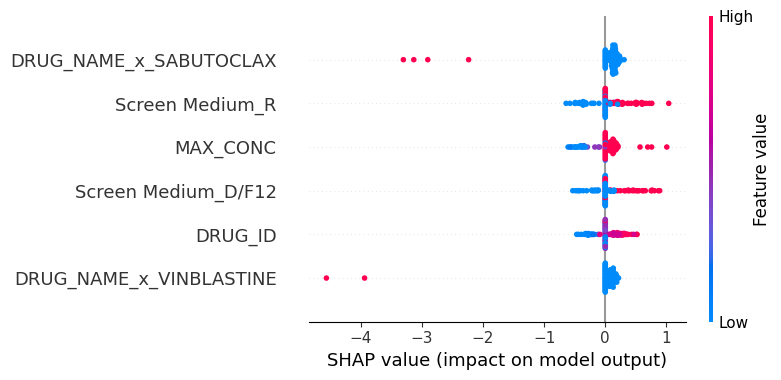
\includegraphics[width=1\textwidth]{figures/shap/shapValuesLittle.png}
        \caption{Example of SHAP values representation: Summary plot with 100 examples.}
        \label{fig:summaryPlot}
    \end{figure}

    \begin{itemize}
        \item Y-axis: The features sorted by relevance.
        \item X-axis: SHAP value. Impact on model output, a positive value show a higher predicton and vice versa.
        \item Dots: Each point represent a record of the dataset.
        \item Color: Indicate the feature value for that example.
    \end{itemize}
    

    \item \textbf{Force plot}: Used for local explainability. It provides the reasons why the prediction is higher or lower for an unique instance. In this type of graph, contrasting colors are used to show how each variable influences the prediction. Features that push the prediction higher are typically shown in red, while those that push it lower are shown in blue. This visualization helps to clearly distinguish between the variables that support and those that oppose the model's output for a specific instance.
    \begin{figure}[H]
        \centering
        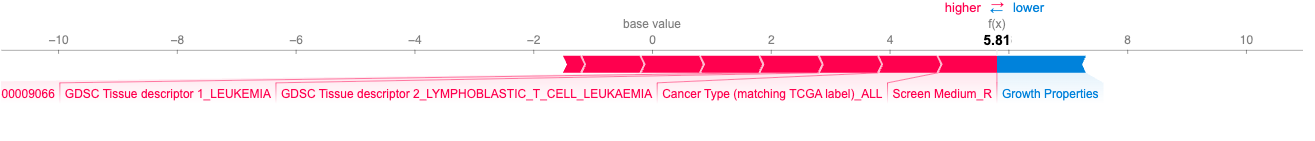
\includegraphics[width=1\textwidth]{figures/shap/force_plot.png}
        \caption{Example of SHAP values representation: Force plot with 100 examples.}
        \label{fig:forcePlot}
    \end{figure}

    Figure~\ref{fig:forcePlot} shows the variables that support increasing the value of the model output, while indicating that the Growth Properties variable is the only one that opposes this increase.

    \item \textbf{Dependence plot}: Used for global explainability. Show how a feature's value affect its SHAP value across the entire dataset helping to identify the relationship.
    \begin{figure}[H]
        \centering
        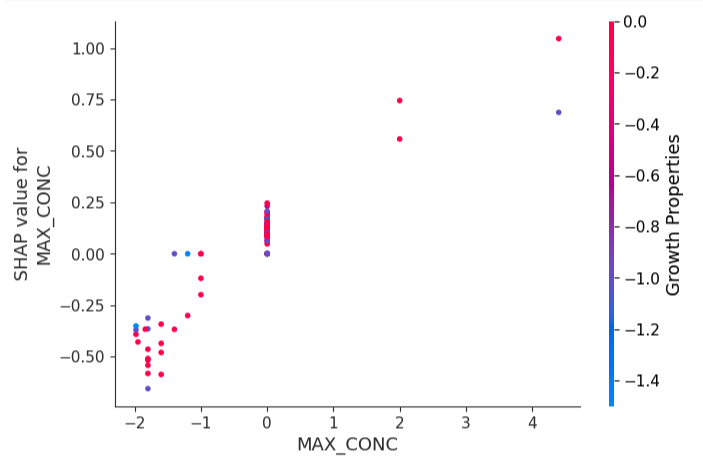
\includegraphics[width=1\textwidth]{figures/shap/depence_plot.png}
        \caption{Example of SHAP values representation: Dependence plot with 100 examples.}
        \label{fig:dependecePlot}
    \end{figure}

    \begin{itemize}
        \item Y-axis: The SHAP value for that variable, how much this feature contiributes to the model's output.
        \item X-axis: The value of the feature.
        \item Color: Indicate the second feature value.
    \end{itemize}

    In the example case shown in Figure~\ref{fig:dependecePlot}, it can be seen that as the MAX\_CONC variable decreases, it contributes less to a positive output, prompting a negative one.
\end{itemize}


    \chapter{Understanding the dataset}\label{cap:analisis}


\section{Introduction}

This research is based on the Genomics of Drug Sensitivity in Cancer (GDSC) dataset, available through Kaggle. The primary aim of this resource is to make publicly available data from the original GDSC repository, with additional annotations to facilitate downstream analysis.

The dataset includes detailed information about various cancer cell lines and their associated types. It provides genomic and molecular features such as mutation status, tissue origin, growth conditions, and methylation patterns. On the pharmacological side, it offers drug-specific information, including treatment response, administered concentrations, and metadata related to drug selection. In addition, it includes a classification label that reflects the effectiveness of the drug response.

Among the most critical variables is the logarithm of the half-maximal inhibitory concentration, denoted as \(LN\_IC_{50}\). This metric quantifies the drug dosage required to inhibit cell viability by 50\%, making it a biologically meaningful and clinically relevant target for prediction. A model capable of accurately predicting \(LN\_IC_{50}\) could serve as a decision-support tool in assigning optimal drug dosages to individual patients. Moreover, gaining insight into the factors that influence this value could offer valuable directions for further research in personalized medicine and oncology.

\section{Description of variables}

The dataset Genomics of Drug Sensitivity in Cancer (GDSC) comprises a total of four files, each providing complementary information on the status of cancer cell lines, patient characteristics, and prescribed medications. One of the most important features of this dataset is that the information it
contains comes from the COSMIC database \cite{cosmic}, one of the most comprehensive
collections on cancer cases and their treatment. In the following sections, each file will be briefly described along with the variables it contains, in order to provide an initial understanding of their relevance and potential utility for this research.

\begin{enumerate}
    \item \textbf{GDSC2-dataset.csv}: Mainly contains information about the medicines used and their effectiveness in the different patients. Among its variables are:
    \begin{itemize}
        \item \textbf{DATASET}: Since the objective of the author of the dataset is to keep the information updated, he uses this variable to indicate which version it comes from, since the database \textit{COSMIC} is updated regularly.
        \item \textbf{NLME\_RESULT\_ID}: Unique identifier of the NLME model to which it is related.
        \item \textbf{NLME\_CURVE\_ID}: Identifier of the dose-response curve fitted by the previous model.
        \item \textbf{COSMIC\_ID}: As its name suggests, this is the identifier by which this record is known in the database \textit{COSMIC}.
        \item \textbf{CELL\_LINE\_NAME}: Name of the cancer cell line of the experiment.
        \item \textbf{SANGER\_MODEL\_ID}: Identifier of the cell used by the Sanger Institute \cite{sanger}.
        \item \textbf{TCGA\_DESC}: Description of the type of cancer according to \textit{The Cancer Genome Atlas}\footnote{Project with the aim of cataloging genomic alterations due to the presence of cancer cells.}.
        \item \textbf{DRUG\_ID}: Identifier of the drug prescribed to the patient.
        \item \textbf{DRUG\_NAME}: Name of the drug used in the treatment.
        \item \textbf{PUTATIVE\_TARGET}: Refers to the original cellular target of the drug, i.e. which cell line the drug is intended to treat.
        \item \textbf{PATHWAY\_NAME}: The biological pathway affected by the drug, i.e., which series of cellular interactions the drug intake modifies.
        \item \textbf{COMPANY\_ID}: Identifier of the company that provides the drug.
        \item \textbf{WEBRELEASE}: Date on which this information was made public on the website.
        \item \textbf{MIN\_CONC}: Minimum used concentration of the drug during follow-up.
        \item \textbf{MAX\_CONC}: Maximum drug concentration used during follow-up.
        \item \textbf{LN\_IC50}: This variable represents the natural logarithm of the $IC_{50}$ value (mean inhibitory concentration). A higher value indicates that a greater dose of the drug is required to achieve the desired effect, suggesting lower sensitivity or resistance. Conversely, a lower value implies that only a small dose was sufficient to produce a significant biological response, indicating higher sensitivity to the drug.
        \item \textbf{AUC}: Area Under the Curve, a statistical measure that in this case reflects the effectiveness of the drug.
        \item \textbf{RMSE}: Error measure known as Root Mean Square Error. It indicates the quality of the dose-response prediction performed by the NLME model.
        \item \textbf{Z\_SCORE}: Standardized performance measure, intended to allow comparisons between different drugs and cell lines.
      \end{itemize}

      \item \textbf{Cell\_Lines\_Details.xlsx}: Contains information about the different cell lines, as well as data related to the patient's cancer. The variables it includes are:
      \begin{itemize}
        \item \textbf{Sample Name}: Unique identifier for the cell line sample.
        \item \textbf{COSMIC identifier}: Unique ID from the COSMIC database for the cell line.
        \item \textbf{Whole Exome Sequencing (WES)}: Genetic mutation data obtained through whole exome sequencing.
        \item \textbf{Copy Number Alterations (CNA)}: Data on gene copy number changes in the cell line.
        \item \textbf{Gene Expression}: Information on gene expression levels in the cell line.
        \item \textbf{Methylation}: Data on DNA methylation patterns in the cell line.
        \item \textbf{Drug Response}: Information on how the cell line responds to various drugs.
        \item \textbf{GDSC Tissue descriptor 1}: Primary tissue type classification. Mainly indicates the type of cancer.
        \item \textbf{GDSC Tissue descriptor 2}: Secondary tissue type classification. It can be interpreted as indicating the region affected by cancer.
        \item \textbf{Cancer Type (matching TCGA label)}: Cancer type according to the TCGA classification.
        \item \textbf{Microsatellite instability Status (MSI)}: Indicates the microsatellite instability status of the cell line.
        \item \textbf{Screen Medium}: Growth medium used to culture the cell line.
        \item \textbf{Growth Properties}: Characteristics of how the cell line grows in culture.
        \end{itemize}

    \item \textbf{Compounds-annotation.csv}: The data in this file refer mainly to the drug:
        \begin{itemize}
            \item \textbf{DRUG\_ID}: Unique identifier for the drug.
            \item \textbf{SCREENING\_SITE}: Location where the drug screening was performed.
            \item \textbf{DRUG\_NAME}: Name of the drug compound.
            \item \textbf{SYNONYMS}: Alternative names for the drug.
            \item \textbf{TARGET}: The molecular target(s) of the drug.
            \item \textbf{TARGET\_PATHWAY}: The biological pathway(s) targeted by the drug.
        \end{itemize}

    \item \textbf{GDSC\_DATASET.csv}: This dataset is the result of preprocessing performed by the original Kaggle author, based on three raw data files included in the same repository. The author applied extensive data cleaning and transformation techniques to reduce noise, enhance signal quality, and incorporate relevant domain knowledge. The resulting file provides a curated version of the data that is ready for analysis and modeling. Among the variables included in this dataset are:
    \begin{table}[H]
        \centering
        \begin{tabular}{|l|l|}
        \hline
        \textbf{COSMIC\_ID} & \textbf{CELL\_LINE\_NAME} \\ \hline
        \textbf{TCGA\_DESC} & \textbf{DRUG\_ID} \\ \hline
        \textbf{DRUG\_NAME} & \textbf{LN\_IC50} \\ \hline
        \textbf{AUC} & \textbf{Z\_SCORE} \\ \hline
        \textbf{GDSC Tissue descriptor 1} & \textbf{GDSC Tissue descriptor 2} \\ \hline
        \textbf{Cancer Type (matching TCGA label)} & \textbf{Microsatellite instability Status (MSI)} \\ \hline
        \textbf{Screen Medium} & \textbf{Growth Properties} \\ \hline
        \textbf{CNA} & \textbf{Gene Expression} \\ \hline
        \textbf{Methylation} & \textbf{TARGET} \\ \hline
        \multicolumn{2}{|c|}{\textbf{TARGET\_PATHWAY}} \\ \hline
        \end{tabular}
        \caption{List of variables present in the GDSC dataset.}
        \label{tab:gdsc_vars}
        \end{table}
\end{enumerate}

Although the preprocessing of the GDSC\_DATASET file is very interesting, its data has not been used for this research. It eliminates some variables that were considered useful for improving the prediction results. For example, including "DRUG\_RESPONSE" among the variables to be predicted could help the model understand some internal relationships in the data. However, given that the procedures applied could be helpful in resolving this research, some of the data provided has been taken into account.


\section{Analyzing the information}

The variable of greatest interest is \(LN\_IC_{50}\), as it is the one that would allow us to know how much medication to administer to the patient. Therefore, the first step is to understand its distribution. This makes it possible to anticipate potential problems understand how it evolves.

\begin{figure}[H]
    \centering
    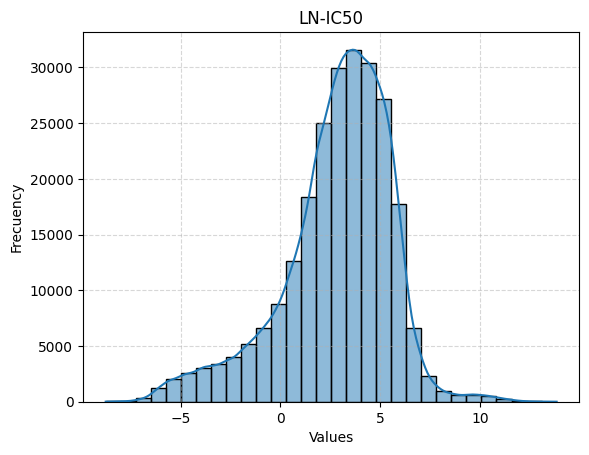
\includegraphics[width=1\textwidth]{figures/LNIC_50_barplot.png}
    \caption{Distribution of the \(LN\_IC_{50}\) variable.}
    \label{fig:lnic50_distribution}
\end{figure}

Figure~\ref{fig:lnic50_distribution} shows how the \(LN\_IC_{50}\) variable follows a normal distribution in which some aspect can be observed:

\begin{itemize}
    \item There are fewer examples on the right side of the distribution, which implies that the data has been slightly skewed when acquiring positive values.
    \item In the same area on the right, a small increase can be seen. This may indicate a population for which more records are available on an ad hoc basis, which could pose a small challenge during model training, as this population disrupts the natural progression of the normal distribution.
    \item In general, it shows good symmetry, thus favouring the training of a model, ignoring the area mentioned above.
\end{itemize}

\subsubsection{Joining the data}

Once the main target variable has been analysed, it is necessary to know how to join the files appropriately so that the records match their corresponding ones. Thus, referring to database terminology, it is necessary to carry out various join operations between the three files, relating each of the foreign keys\footnote{In the context of relational databases, it refers to an identifier that helps link records from one table to records from another.} to their corresponding primary keys.

There are unknown records in each of the three files, so there are several possibilities:
\begin{itemize}
    \item Delete all null values and perform the joins afterwards.
    \item Join the three files and apply value imputation to try to infer the value of the unknown fields.
    \item Join the datasets and then delete the resulting null values.
\end{itemize}

To obtain the complete dataset, it is necessary to merge the GDSC2 and Cell\_Lines\_Details files using  "COSMIC\_ID" and "COSMIC identifier" keys. This is because both records come from different sections of the COSMIC database. The resulting dataset must be linked to Compounds-annotation using the "DRUG\_ID" key, thus obtaining a record with all the data.

When making a decision, it is important to consider that value imputation could improve performance. However, if some of the records are deleted and assigned a status to those that are unknown, the future model could acquire a certain degree of resilience, strengthening the model. Based on this, two decisions were made. Investigate two of the possibilities: on the one hand, the datasets will be joined, applying a process of value imputation a posteriori. On the other hand, null records will be deleted and then the files will be merged. Both resulting datasets will be used in a first regressor to check which data provides the most value. Although this may seem complex, the implementation is straightforward using notebook files\footnote{Development environment that allows you to run code organized in cells}, as the two workflows are nearly identical except for the step involving imputation. This approach will be detailed in a subsequent section.

\subsubsection{Filtering the information}

Applying variable selection procedures reduces the dimensionality of the dataset. This has two key benefits: on the one hand, it reduces noise in the dataset and lowers the computational cost of training the model. On the other hand, it reduces the potential of human error during the initial data collection process. In practical terms, if you only need to record 10 characteristics instead of 20, the likelihood of introducing mistakes during data entry or measurement is significantly lowered.

The current dataset contains many identifiers related to external studies or various databases. These identifiers will not be necessary for this research, meaning that these variables are disposable.

\begin{itemize}
    \item DATASET
    \item NLME\_CURVE\_ID
    \item COMPANY\_ID
    \item COSMIC identifier
    \item Sample Name
    \item COSMIC\_ID
    \item SYNONYMS
\end{itemize}

The next step is to check if any of the variables are obsolete. This condition occurs when all available records for that feature are always the same. To do this, the code described in Listing~\ref{cod:obsoletes} has been used. This makes it possible to identify obsolete variables and determine the size of each variable's domain.

Apparently, the DRUG\_ID and DRUG\_NAME variables contain the same information, so one of them could be discarded. To be sure, it is necessary to check whether there are any inconsistencies in the data and, if so, to determine whether this is due to an error during data collection or whether the information provided is actually important. To check consistency, the function illustrated in Listing~\ref{cod:inconsistencesNameId} has been used. This code systematically scans the dataset to confirm that each drug ID matches its corresponding drug name. In cases where mismatches are detected, the function attempts to identify which variable is inconsistent, providing insight into the source of the discrepancy.

This reveals that there is inconsistency in the names, i.e. some names correspond to more than one identifier. To understand the nature of this inconsistency, the identifiers of the suppliers of these drugs are examined, as they may have a different identifier depending on the supplier. To do this, the code visible in Listing~\ref{cod:supplierConsistence} is used.

\begin{table}[H]
    \centering
    \begin{tabular}{|l|l|l|}
    \hline
    \textbf{Drug Name} & \textbf{Detected IDs} & \textbf{Supplier IDs} \\ \hline
    Docetaxel & [1007, 1819] & [1046, 1043] \\ \hline
    Selumetinib & [1062, 1736] & [1046, 1001] \\ \hline
    Oxaliplatin & [1089, 1806] & [1046, 1043] \\ \hline
    Fulvestrant & [1200, 1816] & [1046, 1043] \\ \hline
    Uprosertib & [1553, 2106] & [1046] \\ \hline
    GSK343 & [1627, 2037] & [1046, 1033] \\ \hline
    Acetalax & [1803, 1804] & [1043] \\ \hline
    Dactinomycin & [1811, 1911] & [1043, 1046] \\ \hline
    Ulixertinib & [1908, 2047] & [1046] \\ \hline
    \end{tabular}
    \caption{Detected inconsistencies between DRUG\_NAME, DRUG\_ID, and their suppliers}
    \label{tab:drug_id_supplier}
\end{table}

Table~\ref{tab:drug_id_supplier} shows that, with the exception of three cases, in all others, when there is an inconsistency between the drug name and its identifier, the medicine is supplied by a different provider. This information can be very useful, as variations between suppliers may involve subtle changes to some component of the drug formula, its preservation or concentration. Therefore, the Drug name and Drug id variables will be retained in the dataset, while the company identifier will be omitted.

\subsubsection{Modifying the representation of data}

Many operations, such as computing correlations, visualizing data, or training machine learning models, require the dataset to be in a numerical format. Therefore, the next step involves transforming categorical variables into numerical representations. A common technique is one-hot encoding; however, this method significantly increases the dimensionality of the dataset, which may negatively affect performance and training time. As an alternative, ordinal encoding will be applied where appropriate, allowing the numerical representation to preserve the inherent order or semantic relationships of the original categories. For example, in a variable representing size with values such as \textit{small}, \textit{medium}, and \textit{large}, assigning them the values 0, 1, and 2, respectively, maintains their natural ordering.

The following variables only express information of Yes, No or unknown value, making them clear candidates for replacement.
\begin{itemize}
    \item Copy Number Alterations (CNA)
    \item Gene Expression
    \item Methylation
    \item Drug Response
\end{itemize}

The Growth Properties variable contains information regarding adhesion, differentiated into three levels: Adherent, Semi-Adherent, and Suspension. Therefore, applying a numerical substitution indicating the degree of adhesion is a plausible option.

Finally, the Screen Medium variable only takes two values, "R" and "D/F12", so instead of applying one-hot encoding, it can be encoded as 0 or 1, depending on which option it is.

In order to facilitate the application of these changes to future data, this entire process is carried out using Sklearn's ColumnTransformer. This class allows you to perform a sequence of transformations on the data easily and effectively. The steps required to do this are illustrated in Listing~\ref{cod:columnTransformer}.

\subsection{Checking the feasibility of assigning values}

The imputation of unknown values could improve results, which is why research has been conducted on this topic. The objective is to conduct a small test to verify whether imputing values improves accuracy or whether, on the contrary, allowing a certain degree of ambiguity in the data improves the robustness of the model. To achieve this, the steps described below have been followed.

To perform the imputation process, all variables must be numbers. However, after the preprocessing described above, the dataset retains some categorical features. Since these variables cannot be expressed in numerical format while maintaining the relationship between them, the ideal solution would be to apply a one-hot encoder, but this would significantly increase the computational cost of applying value imputation. Therefore, Sklearn's ordinal encoder \cite{scikit-learn-ordinalencoder} has been used, which allows categorical variables to be replaced by numerical ones, while maintaining the correspondence stored, in case it needs to be restored later. This process can be observed in Listing~\ref{cod:ordinalEncoder}.

Once the dataset does not contain categorical information, it is possible to apply imputation methods. During this research, the method selected was KNNImputer \cite{scikit-learn-knnimputer}, which creates clusters between the data and imputes values based on the nearest centroids. In other words, it assigns values based on their similarity to known data. The application of this technique can be seen in Listing~\ref{cod:knnImputer}.

\subsubsection{Comparing results}

Comparing the results between applying value imputation and assigning values to nulls after the unification process will allow us to determine which method is best for the research.

To perform the comparison, a neural network architecture consisting of three fully connected (dense) layers was implemented, as detailed in Listing~\ref{cod:pythonGenerateNet}v. This structure was chosen to ensure a fair and consistent baseline for evaluating the impact of preprocessing. The network was trained using both datasets, one with imputed values and one without. The results from each training scenario were then collected and analyzed to assess the influence of the imputation step on model performance.

\begin{table}[H]
    \centering
    \begin{tabular}{|c|c|}
    \hline
    \textbf{Metric} & \textbf{Value} \\
    \hline
    MSE  & 0.843 \\
    RMSE & 0.918 \\
    MAE  & 0.674 \\
    \hline
    \end{tabular}
    \caption{Model performance in the test set after applying value imputation.}
    \label{tab:model_metrics_imputing_values}
\end{table}

\begin{table}[H]
    \centering
    \begin{tabular}{|c|c|}
    \hline
    \textbf{Metric} & \textbf{Value} \\
    \hline
    MSE & 0.320 \\
    RMSE & 0.566 \\
    MAE & 0.300 \\
    \hline
    \end{tabular}
    \caption{Model performance in the test set without applying value imputation.}
    \label{tab:test_metrics_without_values_imputation}
\end{table}

As can be seen in Tables~\ref{tab:model_metrics_imputing_values} and \ref{tab:test_metrics_without_values_imputation}, the model's performance is severely compromised after applying value imputation. Everything seems to indicate that adding some ambiguity to the data does indeed make the model more robust and versatile.

    \chapter{In search of solutions}\label{cap:diseño}

\section{Solving our regression problem}

The estimation of the variable \(LN\_IC\_{50}\) is considered highly beneficial in the fight against cancer. If this value can be accurately predicted, cases in which excessive medication is prescribed, potentially harming the patient's system, could be avoided. Patients requiring higher doses could be identified, thereby improving their outcomes during the course of the disease. To achieve this goal, it is essential that the target variables provided in the dataset are considered. Even if they are not all the primary objective, they can support the learning process of the algorithm, enabling more comprehensive and accurate predictions.

In line with this approach, the selected target variables, besides the \(LN\_IC\_{50}\) indicator, include the AUC curve, RMSE value, Z-Score, and the Boolean drug response. These variables contribute to understanding the behavior and characteristics of \(LN\_IC\_{50}\) across various blood samples, drugs, cancer types and other factors. Despite the preprocessing already performed, many variables still remain unordered or categorical in nature, such as blood samples, drug names or tissue descriptors. Therefore, one-hot encoding\footnote{This is a method for converting categorical data into numerical format. Instead of assigning arbitrary numeric values to categories, one-hot encoding creates a binary vector for each category \cite{amit2024onehot}.} will be applied to these features. This will be done using the get\_dummies function from the pandas library, which is already being utilized for various other operations. However, this transformation may be viewed as controversial, since it significantly increases the dataset's dimensionality, from 21 variables to 1339.

The next step to prepare the data for model training, is to divide it into three distinct subsets: a training set, a validation set and a test set. This division helps ensure that the model learns from one portion of the data the training set, while its performance is periodically evaluated on a separate subset the validation set, reducing the risk of overfitting. During training, the model attempts to minimize error on the training data, but its hyperparameters and general behavior are refined based on its performance on the validation set. Finally, once the model is fully trained, its ability to generalize is assessed using the test set, since it is a collection of data it has never seen before. This evaluation provides an unbiased estimate of the model's performance on new unseen data.

Although this step may appear straightforward, it is indispensable. It is essential to ensure that these subsets are representative of the overall data distribution. If the data is split in an unsupervised or careless manner, it may result in certain populations being excluded from the training set. This, in turn, would hinder the model's ability to learn from those data groups and ultimately reducing the generalization capacity of the model.

Therefore, after separating the data using sklearn's train\_test\_split method \cite{scikit-learn-train-test-split}, the various distributions have been represented using bar charts. This allows to check the differences between the distributions in order to detect anomalies between them.

\begin{figure}[H]
    \centering
    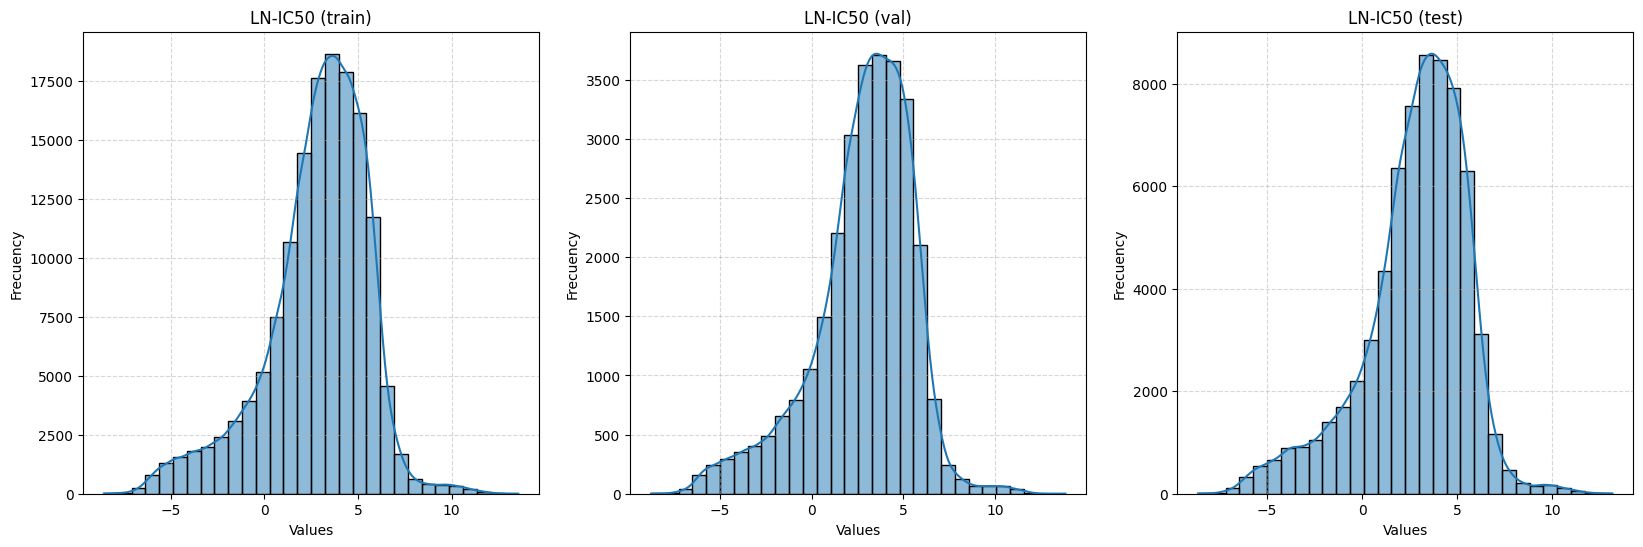
\includegraphics[width=1\textwidth]{figures/data_representation/LNIC50-splits.png}
    \caption{Distributions of the variable \(LN\_IC_{50}\) in the different subsets.}
    \label{fig:lnic50Split}
\end{figure}

\begin{figure}[H]
    \centering
    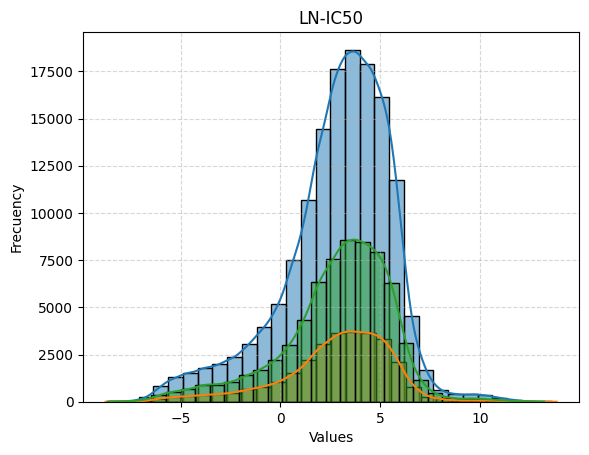
\includegraphics[width=1\textwidth]{figures/data_representation/LNIC50-splits-joined.png}
    \caption{Distributions of the variable \(LN\_IC_{50}\) in the different subsets represented in the same graph to facilitate comparison.}
    \label{fig:lnic50SplitJoined}
\end{figure}

In order to achieve better results, the data can be standarize. This process involves representing all the information on the same scale, i.e. which is specially important for algorithms like neural networks. Scikit-learn provides severals functions for this purpose, such as the StandardScaler \cite{scikit-learn-standardscaler}, which use the mean and the standar desviation to standarize the data.

The transformation applied by \texttt{StandardScaler} follows the formula:

\[
x' = \frac{x - \mu}{\sigma}
\]

Where \( x \) is the original value, \( \mu \) is the mean of the feature, and \( \sigma \) is the standard deviation.

Although the \texttt{StandardScaler} is widely used in many research studies, in this work it was decided to choose to use the \texttt{RobustScaler} \cite{scikit-learn-robustscaler} instead. This method has two main advantages: it standardizes the data while also reducing the influence of noise in the dataset. In particular, it is less sensitive to outliers, which is a highly valuable property when it is necessary to avoid misleading trends caused by extreme values. \texttt{RobustScaler} applies the formula:

\[
x' = \frac{x - \text{median}(x)}{\text{IQR}(x)}
\]

\[
\text{IQR}(x) = Q_3(x) - Q_1(x)
\]

Where \(x\) is the original value, \(x'\) is the scaled value, \(median(x)\) is the median of that feature and \(IQR\) is the interquartile range\footnote{The difference between the first and the last quartile.}. 

Given their proven effectiveness in similar contexts, both neural networks and XGBoost are selected as candidate algorithms for model training.
\begin{itemize}
    \item \textbf{Neural networks}: Neural networks are well-suited for handling high-dimensional data and typically outperform other algorithms in such contexts. In addition, applying convolutional layers could improve this predictive performance, by capturing local patterns or dependencies between related samples. This is particulary relevant, as the main aim to uncover potential relationships between blood samples, the drugs and the cancer react.
    \item \textbf{XGBoost}: Tree based model used to get great performance with tabular data, even they are able to overcome or match deep learning algorithms, like neural networks \cite{treesOverNets}. Moreover, training a tree-based model is typically faster and easier, compared to training a neural network, which takes more time. Another key advantage is interpretability, as tree models provide clearer insights into decision-making processes. However, they have one notable disadvantage: they are not able to extrapolate beyond the range of the train data due to how the algorithm learn \cite{treesLimitations}.
\end{itemize}

\subsection{Predicting $LN\_IC_{50}$ using Neural Networks}

Tensorflow is the framework selected for this reasearch due to it provides a smooth learning curve and includes built-in tools which helps to visualize the architecture and training progress.

During this research the following callbacks\footnote{Callbacks are functions or routines that are automatically called at specific points during training, such as at the end of an epoch or after a batch. They are commonly used for tasks like saving models, early stopping, adjusting the learning rate or logging training metrics.} will be used:
\begin{itemize}
    \item PlotLossesKerasTF \cite{livelossplot}: This package allows real-time visualization of training loss and other metrics during model training.
    \item ModelCheckpoint \cite{modelcheckpoint}: This callback save the best-performing model based on a chosen evaluation metric.
    \item EarlyStopping \cite{earlystopping}: Sometimes the model is not able to learn more. In this situations is common that the validation loss does not improve. When the moment in captured, the training is stopped using this callback. This enables to reduce the training time and to avoid overfitting. There are some occasions, where the model is not able to improve the validation results after a few epochs. In order to fix this, the callback needs patience of 10 epoch.
    \item ReduceLROnPlateau \cite{reducelronplateau}: Similar to the last one, this callback point out, in case the model stop of learning. In that moment it reduces the leaning rate in order to get an improvement in validation results. The patience considered was 7, as when this callback is applied the improvement is slower.
\end{itemize}



\subsubsection{Comparison of loss functions}

One of the main hyperparameters\footnote{A configuration variable set before training, which often determines whether the model learns effectively.} that must be configured during model development is the loss function. The choice of an appropriate loss function can significantly influence the quality of the results. Therefore, a function that aligns well with the nature of the problem should be selected. In this context, three potential candidates have been considered:

\begin{itemize}
    \item \textbf{MSE \cite{tensorflow-mse} (Mean Squared Error)}: Measures the averages squared difference between predicted values \(\hat{y}\) and the real ones \(y\). It is sensitive to large errors, but also to outliers. Sice the units are sqaured is less interpretable than other metrics like RMSE \cite{tensorflow-rmse}.
    \[
    \text{MSE} = \frac{1}{n} \sum_{i=1}^{n} (y_i - \hat{y}_i)^2
    \]

    \item \textbf{logCosh \cite{tensorflow-logcosh}}: It combines the best of MSE and MAE \cite{tensorflow-mae}, it is les sensitive to outliers and smoother than MAE. This function follows the formula:
    \[
    \text{LogCosh}(y, \hat{y}) = \sum_{i=1}^{n} \log\left( \cosh(\hat{y}_i - y_i) \right)
    \]

    This means in small errors it works like MSE and in the large ones, it grows more slowly like MAE. In addtion, it is derivable in all his domain, which ideal for neural network training.

    \item \textbf{Huber \cite{tensorflow-huber}}: This loss function try to replicate the principes of LogCosh, it works as squared error when this one is low, and it is linear for large errors. It requires tunning one hyperparameter, \(\delta\).
    \[
    L_{\delta}(y, \hat{y}) =
    \begin{cases}
    \frac{1}{2}(y - \hat{y})^2 & \text{if } |y - \hat{y}| \leq \delta \\
    \delta \cdot (|y - \hat{y}| - \frac{1}{2} \delta) & \text{otherwise}
    \end{cases}
    \]

\end{itemize}

\subsubsection{Development of our regressor model}

In order to determine the most appropriate approach for the research, some of methods were defined to increase the dynamism of the research. These can be found in the appendix in Listing~\ref{cod:pythonGenerateNet}, \ref{cod:pythonCompileNet} and \ref{cod:pythonShowMetrics}.


By default, the RMSE will be displayed during our training, just to interpret the learning progress.

\subsubsection{Getting the tools to compare error functions}

The initial training was conducted using Mean Squared Error (MSE) as the loss function. While simple, MSE is one of the most effective metrics for gaining insight into how well the model is learning during the early stages of training.

The training progress is illustrated in Figure~\ref{fig:mse_reg_net_train}.

\begin{figure}[H]
    \centering
    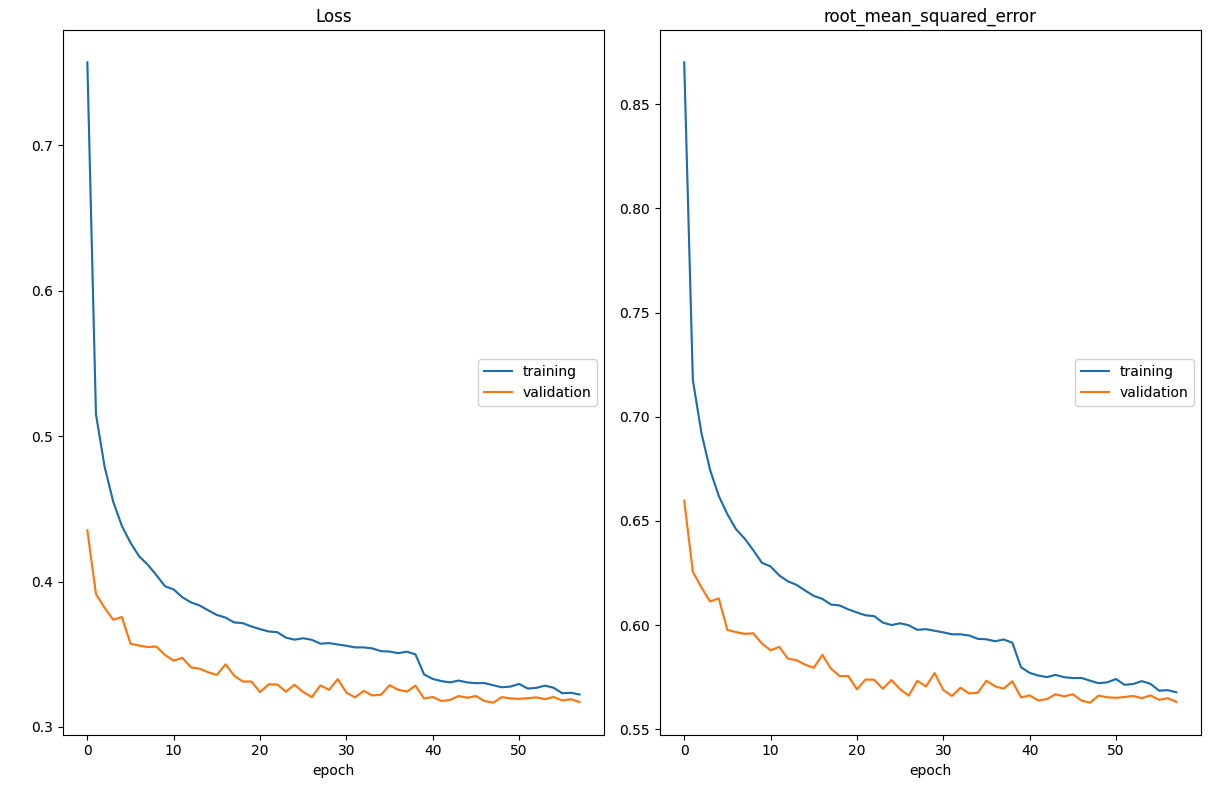
\includegraphics[width=1\textwidth]{figures/neural_net_regression_research/train_mse_neural_net.png}
    \caption{Study of the feasibility of employing MSE as a loss function using a neural network.}
    \label{fig:mse_reg_net_train}
\end{figure}

A summary of the training and validation performance, in terms of loss and RMSE, is provided in Table~\ref{tab:loss-rmse}, which shows the final values of the loss function and RMSE at the end of training.


\begin{table}[ht]
    \centering
    \begin{tabular}{|c|c|}
    \hline
    \textbf{Metric} & \textbf{Best value} \\
    \hline
    Loss (validation) & 0.317 \\
    RMSE (validation) & 0.563 \\
    \hline
    \end{tabular}
    \caption{Training and validation performance summary (loss and RMSE).}
    \label{tab:loss-rmse}
\end{table}

Finally, the overall performance of the model on the evaluation dataset is summarized in Table~\ref{tab:test_metrics_mse}:

\begin{table}[H]
    \centering
    \begin{tabular}{|c|c|}
    \hline
    \textbf{Metric} & \textbf{Value} \\
    \hline
    MSE & 0.320 \\
    RMSE & 0.566 \\
    MAE & 0.300 \\
    R\textsuperscript{2} & 0.575 \\
    \hline
    \end{tabular}
    \caption{Performance metrics on the test set using MSE as loss function.}
    \label{tab:test_metrics_mse}
\end{table}

Figure~\ref{fig:mse_reg_net_result} illustrates the relationship between the predicted values generated by our model and the corresponding actual values. In an ideal scenario, all points would lie precisely on the red diagonal line, which represents perfect predictions. Although not all predictions fall exactly on this line, the majority are closely clustered around it, indicating a generally good predictive performance. However, it is worth noting that in cases where the actual values are particularly high, the model tends to underpredict, suggesting a limitation in capturing extreme values accurately.

\begin{figure}[H]
    \centering
    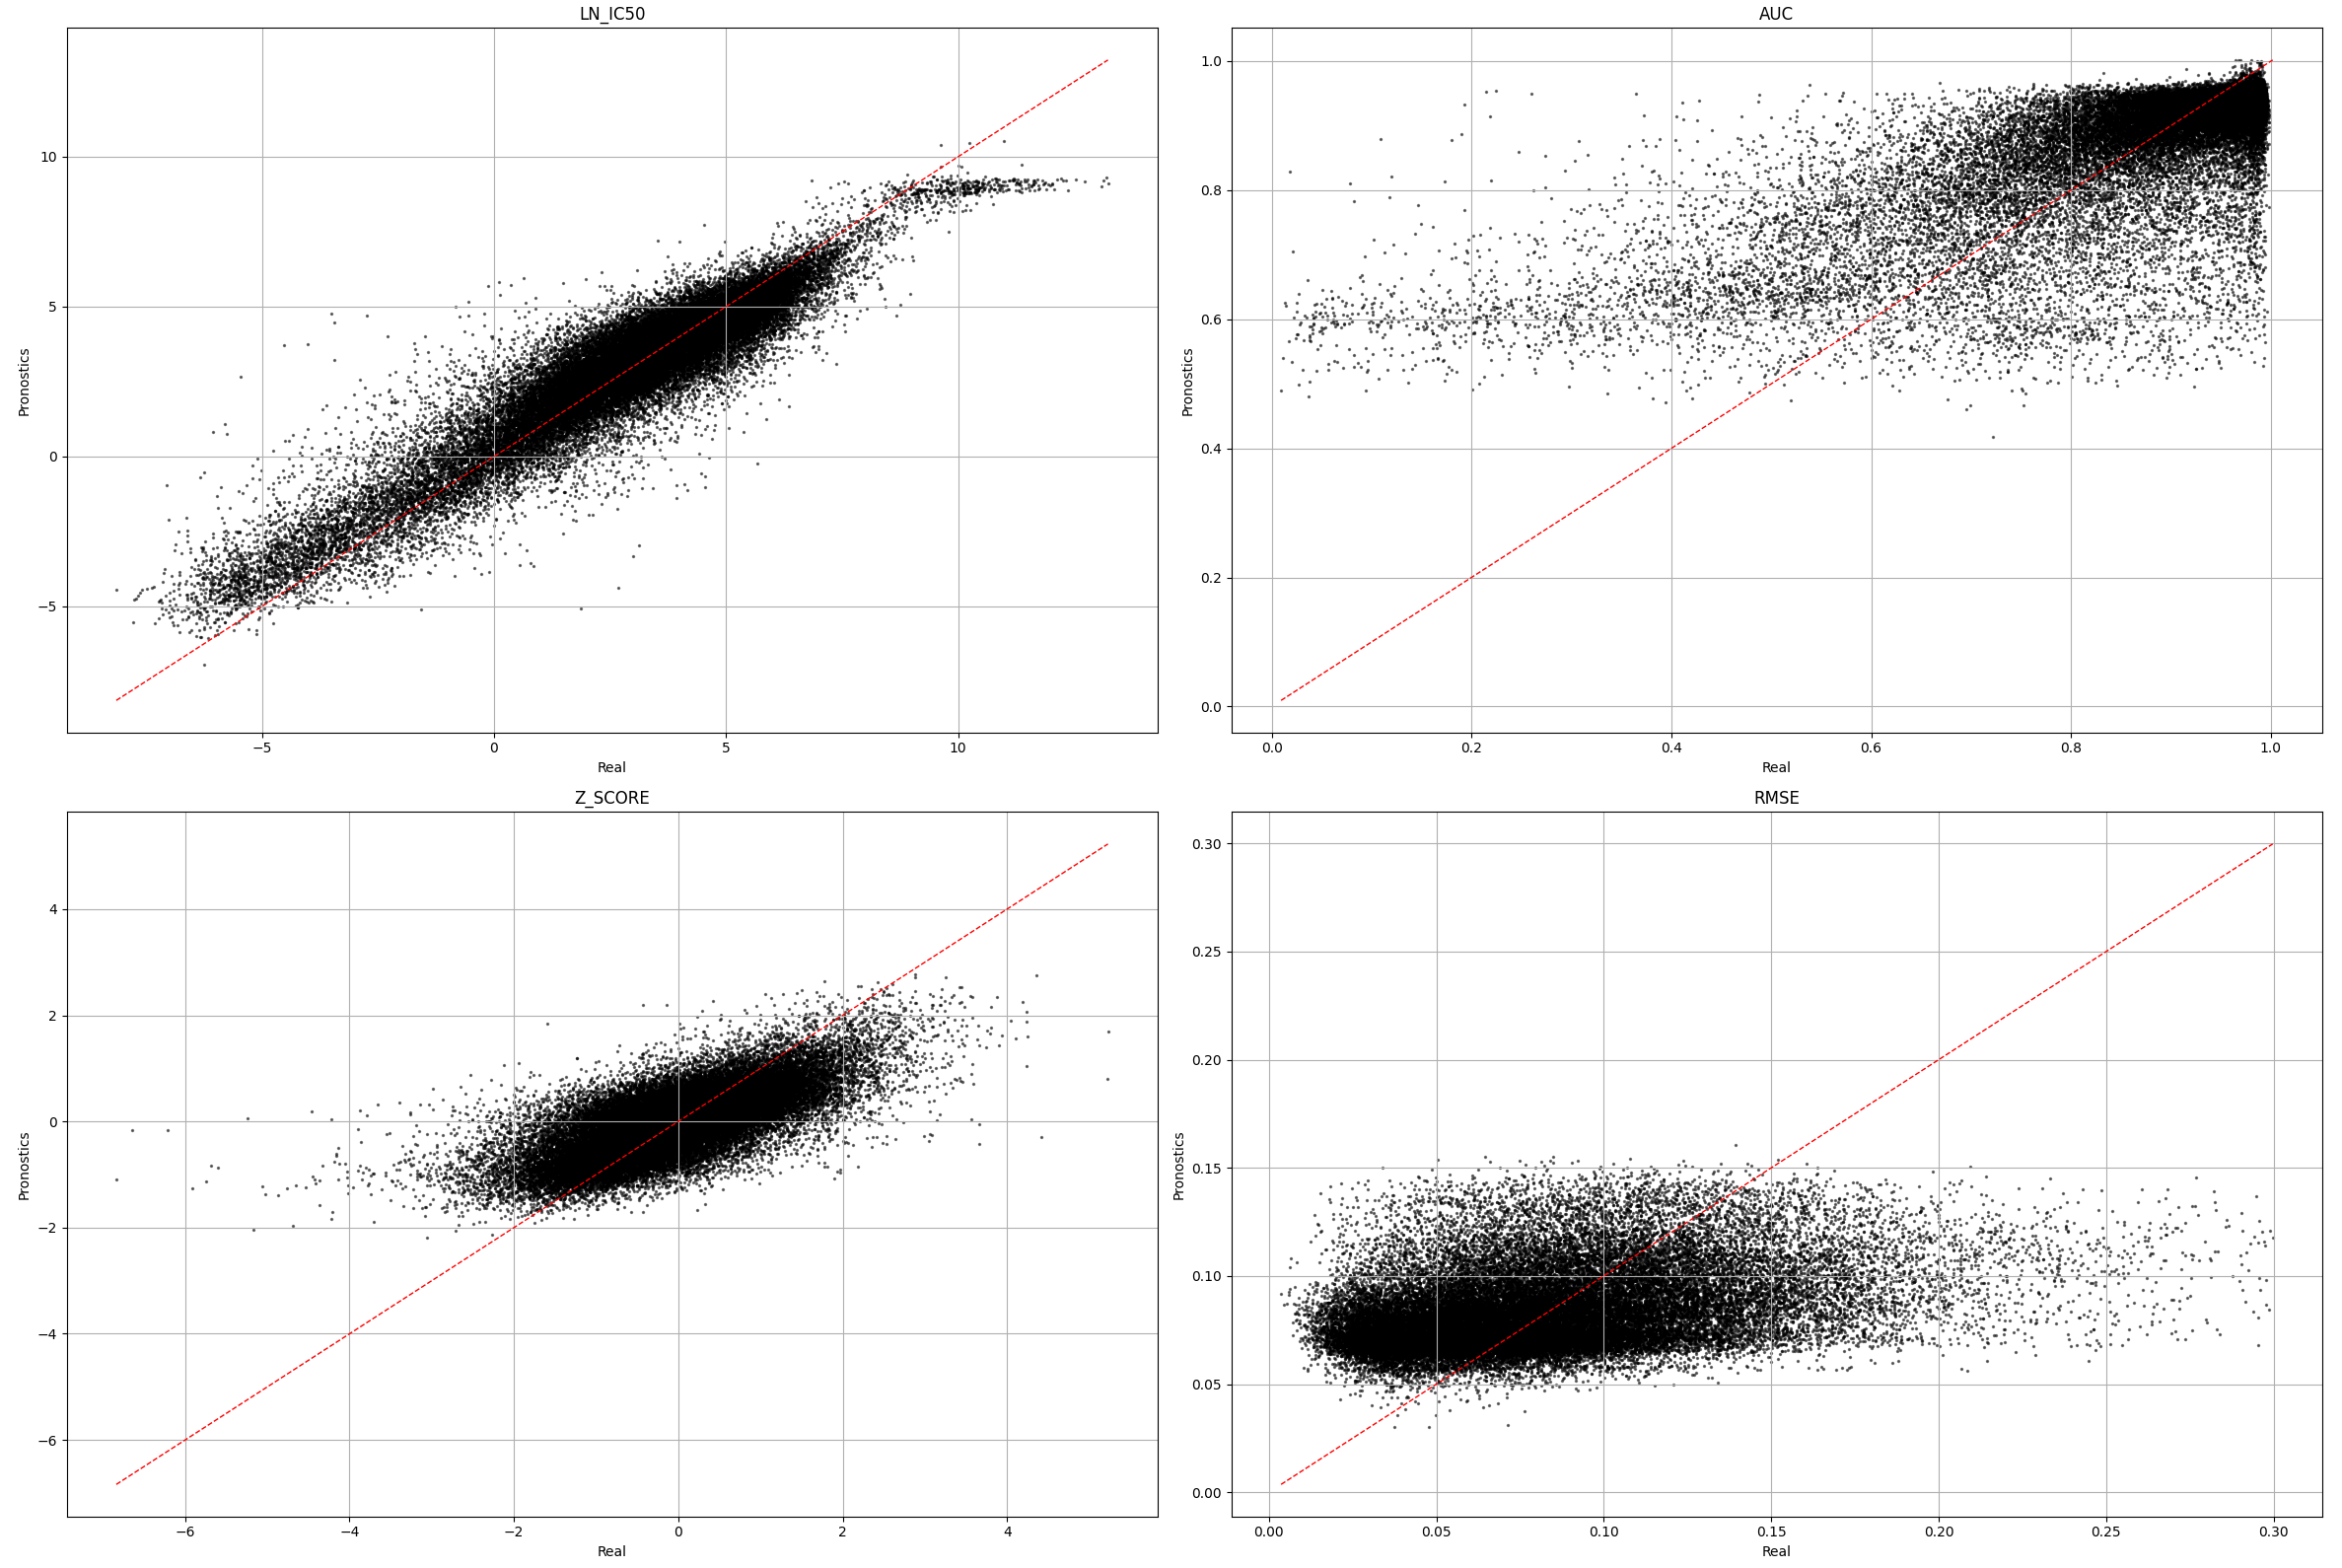
\includegraphics[width=1\textwidth]{figures/neural_net_regression_research/output_neural_net_mse.png}
    \caption{Result of employing MSE as a loss function using a neural network.}
    \label{fig:mse_reg_net_result}
\end{figure}

To further the research, the same process will be repeated with LogCosh as loss function. This could be a nice alternative because it works better with outliers than MSE and also it has a good performance with small error. For this reasons this one could be a great alternative.

In Figure~\ref{fig:logcosh_reg_net_train} si displayed the difference between training and validation, something similar to what it was seen in Figure~\ref{fig:mse_reg_net_train}. But there is a clear difference, in the previous case it seems that the model is not able to learn more, while in this one more fluctuations can be observed during learning, which allow us to see how each time the model makes a mistake and increases the error, it rectifies in the next step. This change is due to the new loss function. While ReLU is unable to represent negative values, LogCosh can. 

\begin{figure}[H]
    \centering
    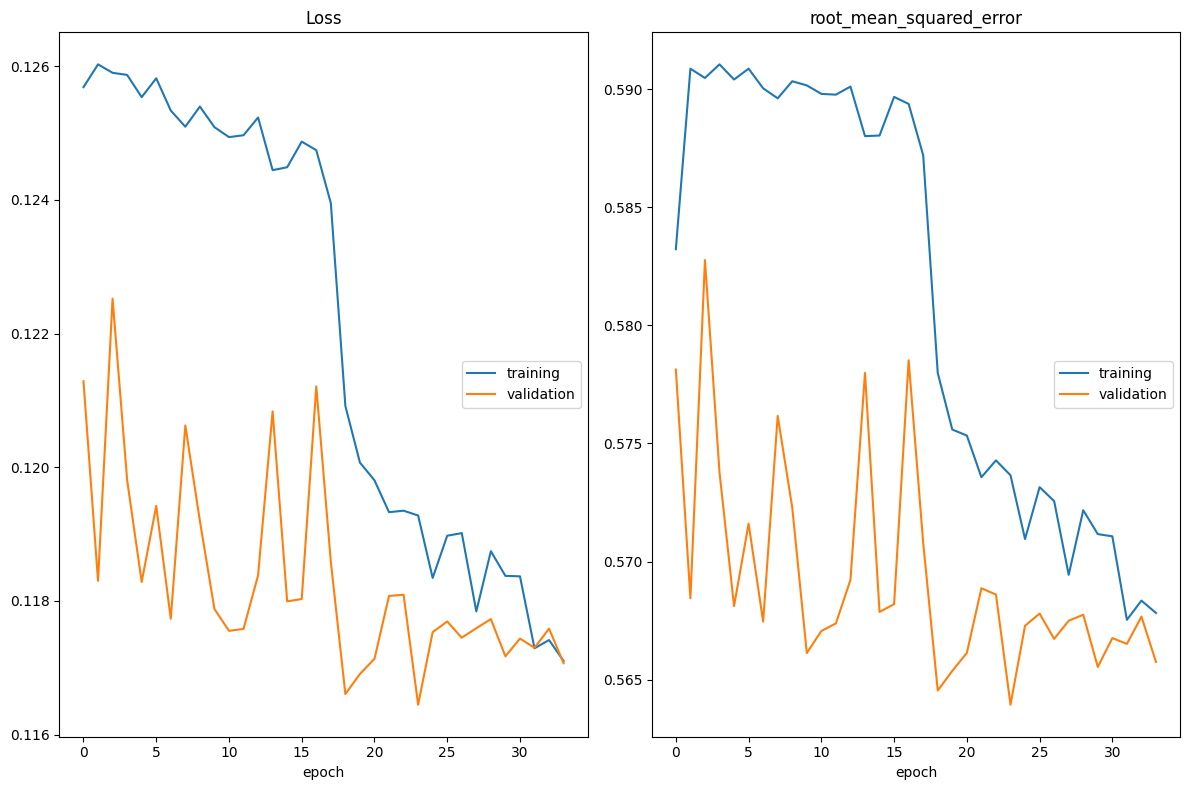
\includegraphics[width=1\textwidth]{figures/neural_net_regression_research/train_logcosh_net.png}
    \caption{Study of the feasibility of employing logarithm of the hyperbolic cosine as a loss function using a neural network.}
    \label{fig:logcosh_reg_net_train}
\end{figure}

In this case the predictions over the test set were a little bit worse that the previous one. 

\begin{table}[h]
    \centering
    \begin{tabular}{|c|c|}
    \hline
    \textbf{Metric} & \textbf{Best value} \\
    \hline
    Loss (validation) & 0.116 \\
    RMSE (validation) & 0.564 \\
    \hline
    \end{tabular}
    \caption{Validation performance metrics at the end of training using LogCosh.}
    \label{tab:loss-rmse-validation}
\end{table}

\begin{table}[H]
    \centering
    \begin{tabular}{|c|c|}
    \hline
    \textbf{Metric} & \textbf{Value} \\
    \hline
    MSE & 0.321 \\
    RMSE & 0.567 \\
    MAE & 0.299 \\
    R\textsuperscript{2} & 0.577 \\
    \hline
    \end{tabular}
    \caption{Performance metrics on the test set using LogCosh as loss function.}
    \label{tab:test_metrics_logcosh}
\end{table}

Although at first glance the results shown in Figures~\ref{fig:mse_reg_net_result} and \ref{fig:logcosh_reg_net_result} may appear nearly identical, a more in depth analysis reveals key differences. In Figure~\ref{fig:mse_reg_net_result}, the model trained with MSE appears to exhibit slightly less dispersion in its predictions, as the plot presents a more defined shape compared to that of Figure~\ref{fig:logcosh_reg_net_result}.

However, the evaluation of training progress tells a different story. In Figure~\ref{fig:mse_reg_net_train}, it can be observed that after only a few training iterations, the model reaches a plateau, showing little to no further improvement, an indication of early stagnation. In contrast, Figure~\ref{fig:logcosh_reg_net_train} displays a continued downward trend in the loss function, even in the final training stages. This suggests that the model trained with Log-Cosh loss retains the potential for further optimization, making it a more promising candidate than the one trained with MSE.


\begin{figure}[H]
    \centering
    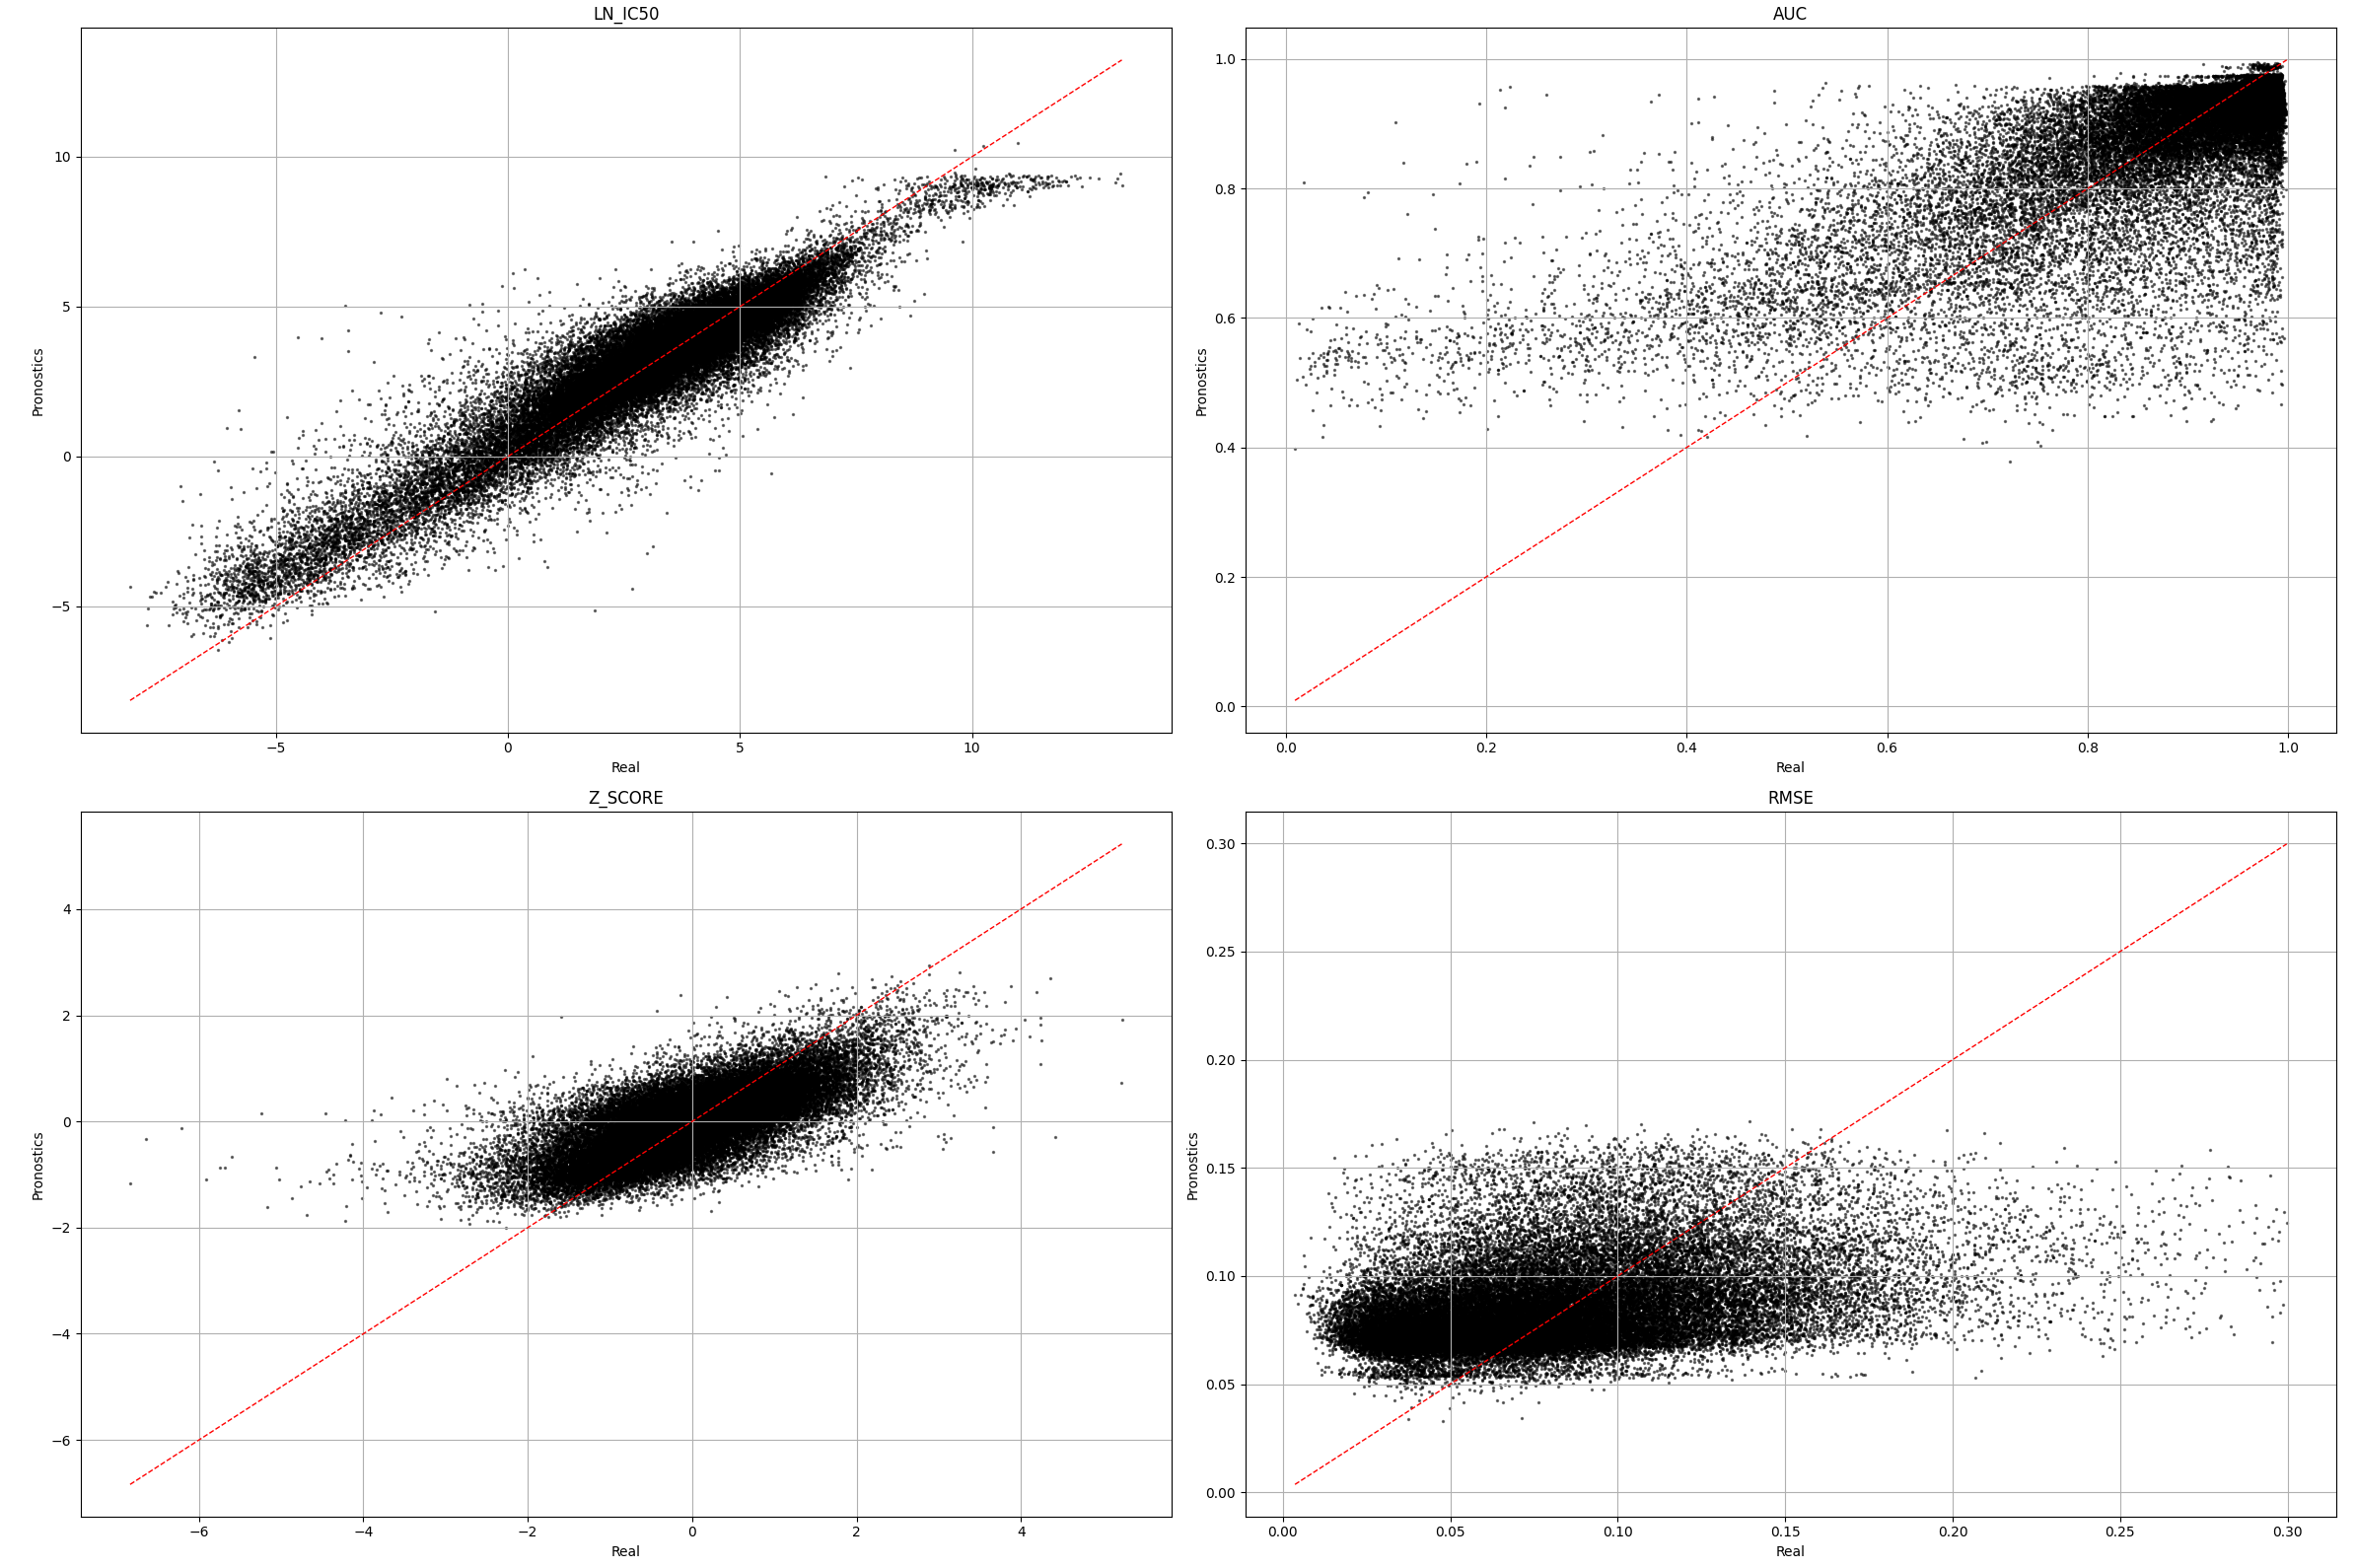
\includegraphics[width=1\textwidth]{figures/neural_net_regression_research/output_neural_net_logcosh.png}
    \caption{Result of employing logarithm of the hyperbolic cosine as a loss function using a neural network.}
    \label{fig:logcosh_reg_net_result}
\end{figure}

Finally, a new model is trained using the Huber loss function. Just as a reminder, this function and LogCosh have similar target but different points of views. The both are robust to reduce the impact of outliers, but this one require one hyperparameter, \(\delta\), which one is used as thresshold.



\begin{figure}[H]
    \centering
    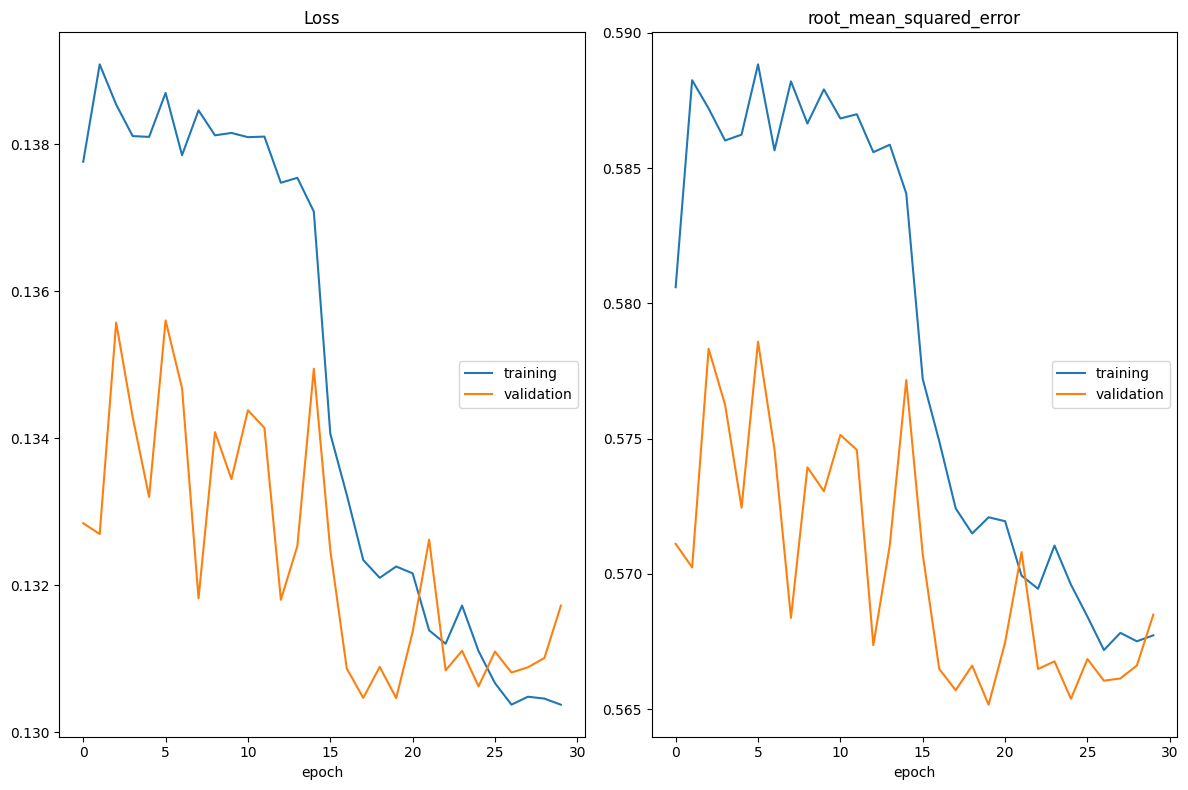
\includegraphics[width=1\textwidth]{figures/neural_net_regression_research/train_huber_net.png}
    \caption{Study of the feasibility of employing Huber as a loss function using a neural network.}
    \label{fig:huber_reg_net_train}
\end{figure}

\begin{table}[h]
    \centering
    \begin{tabular}{|c|c|}
    \hline
    \textbf{Metric} & \textbf{Best value} \\
    \hline
    Loss (validation)  & 0.130 \\
    RMSE (validation)  & 0.565 \\
    \hline
    \end{tabular}
    \caption{Validation performance metrics at the end of training using Huber loss.}
    \label{tab:loss-rmse-validation-huber}
\end{table}

\begin{table}[H]
    \centering
    \begin{tabular}{|c|c|}
    \hline
    \textbf{Metric} & \textbf{Value} \\
    \hline
    MSE & 0.321 \\
    RMSE & 0.567 \\
    MAE & 0.297 \\
    R\textsuperscript{2} & 0.586 \\
    \hline
    \end{tabular}
    \caption{Performance metrics on the test set using Huber as loss function.}
    \label{tab:test_metrics}
\end{table}


At the beginning of the training, the model trained with the Huber loss function seems really interesting, since, as illustrated in Figure~\ref{fig:huber_reg_net_train}, the results on the validation set are better than on the training set, a sign that the network is able to generalise certain behaviours. However, as the epochs go by, this difference not only reduces but the validation error exceeds the train error, gradually acquiring a clear upward trend, as can be seen in the same figure. This represents a major drawback, since if the model does not acquire or loses the ability to generalise, the results provided by the model are worthless, as it is not able to understand the nature of the progression.

\begin{figure}[H]
    \centering
    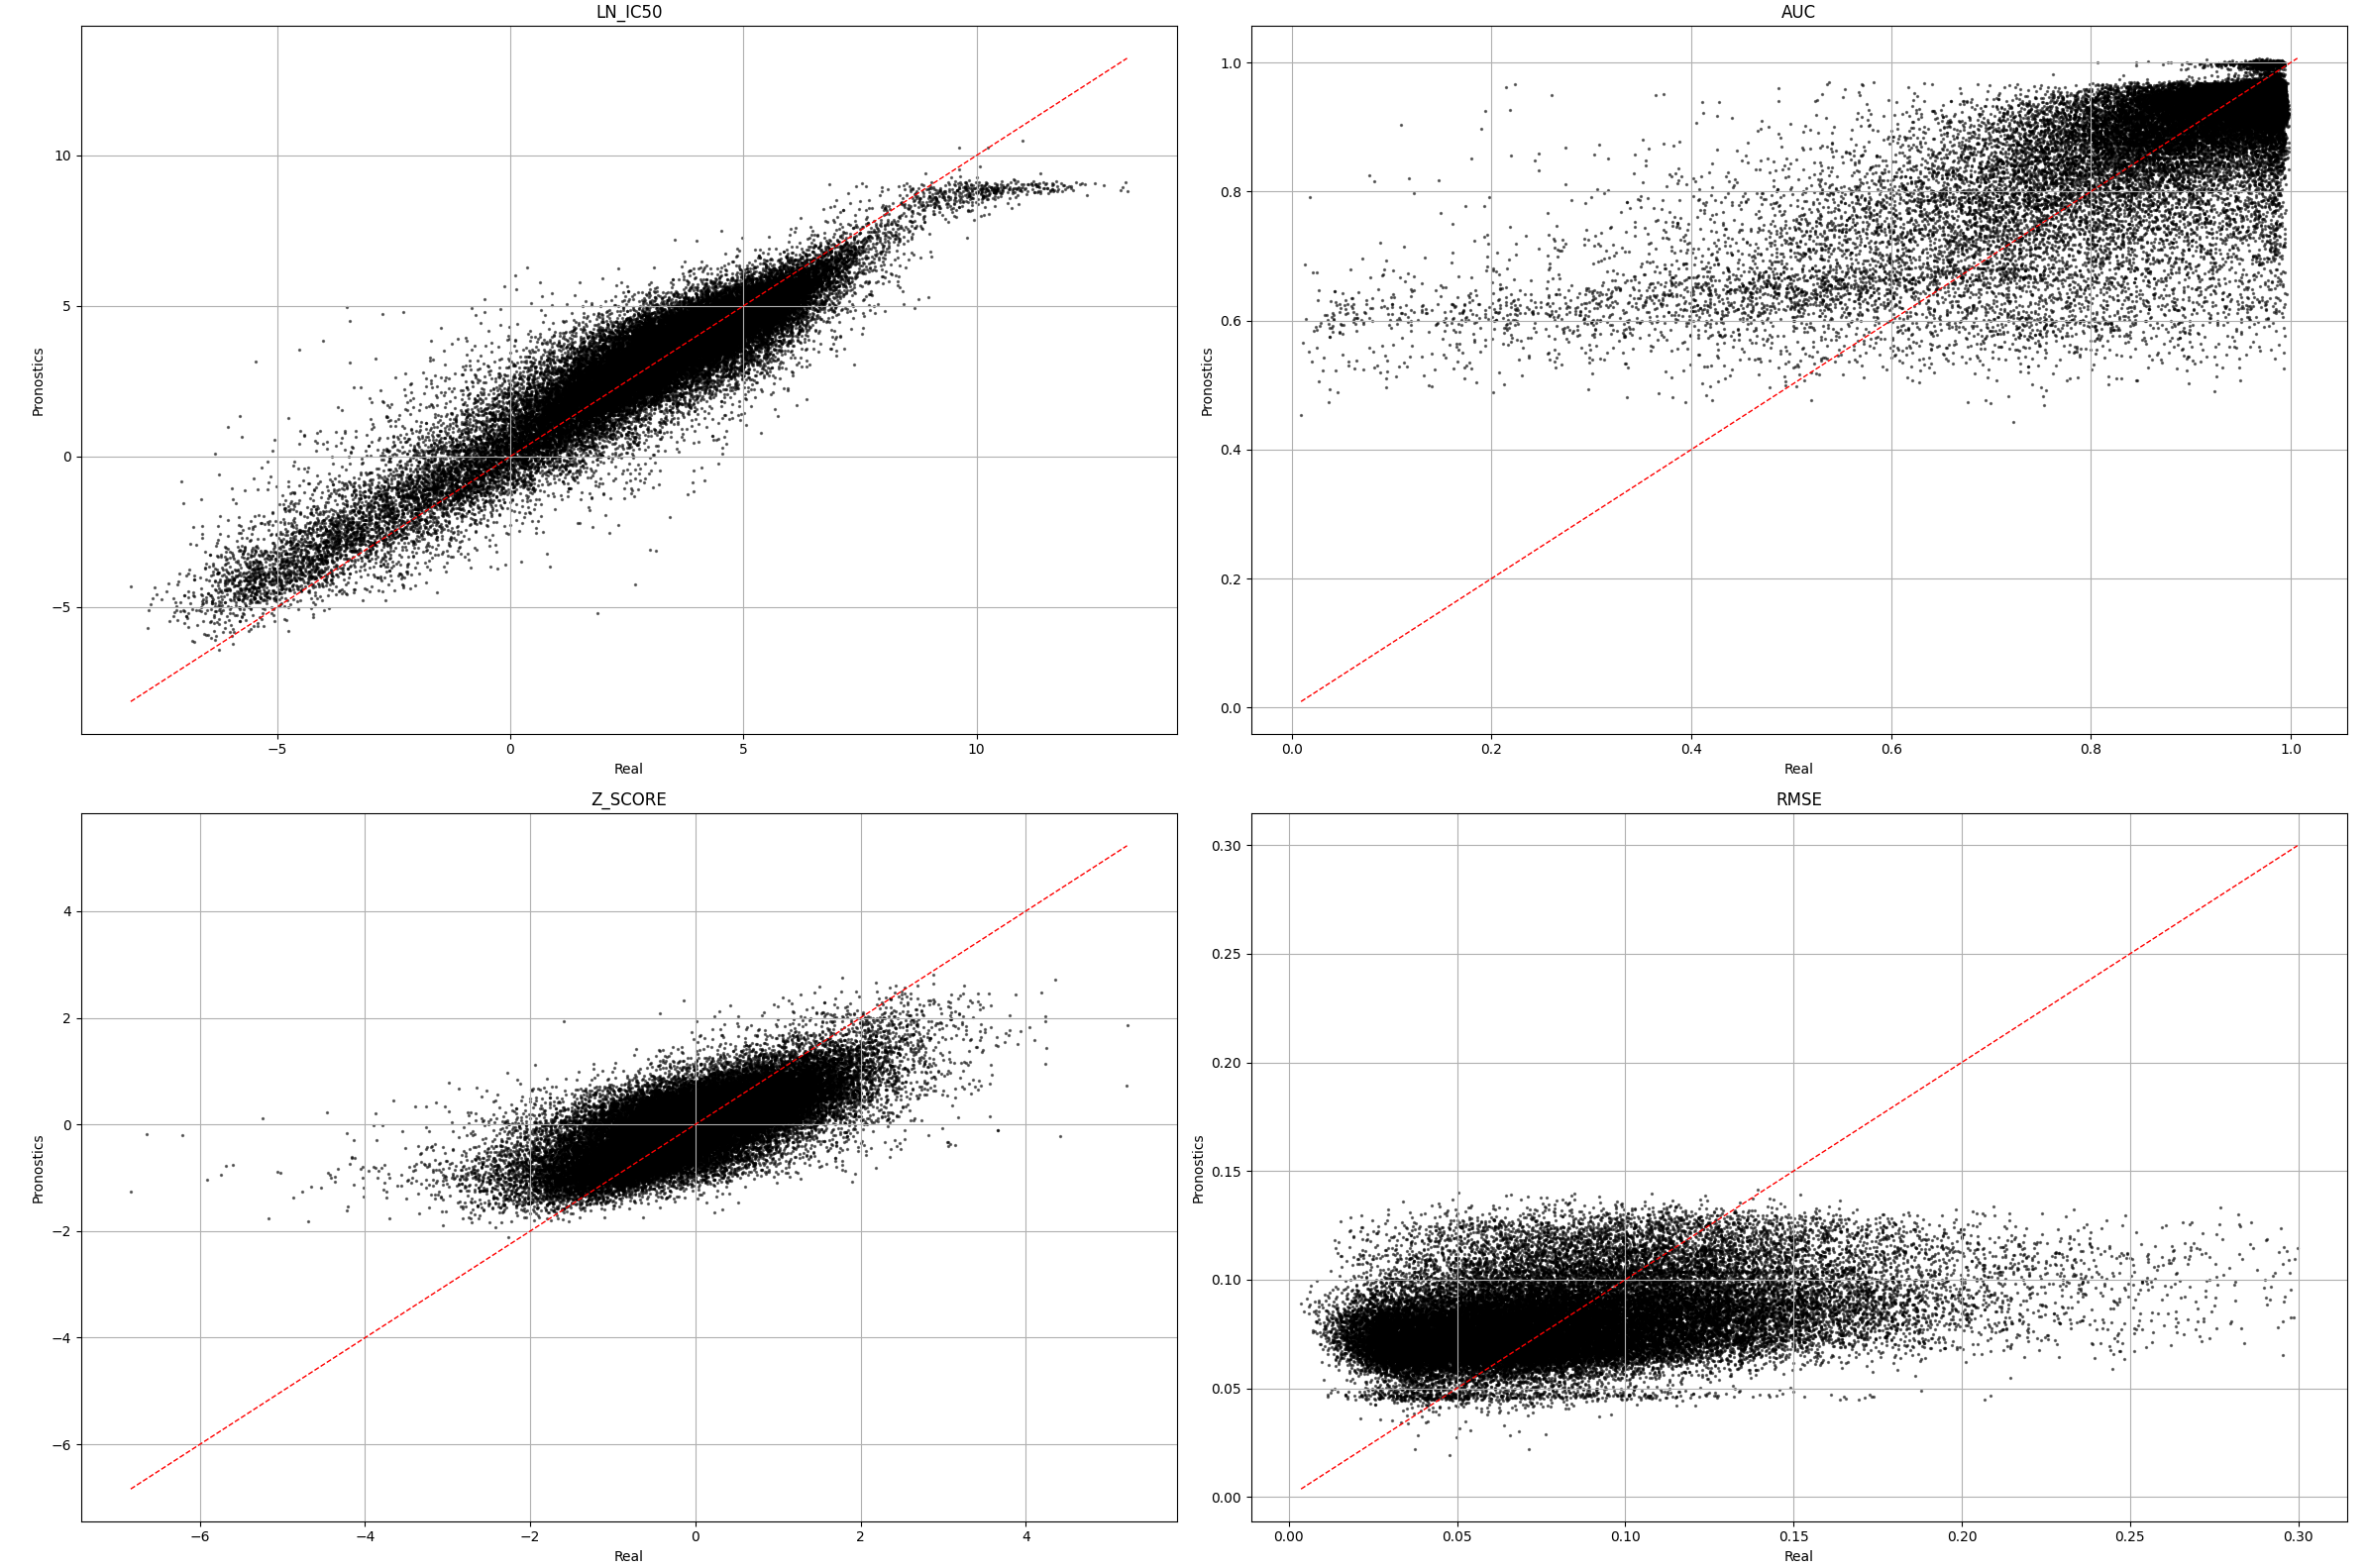
\includegraphics[width=1\textwidth]{figures/neural_net_regression_research/output_neural_net_huber.png}
    \caption{Result of employing Huber as a loss function using a neural network.}
    \label{fig:huber_reg_net_result}
\end{figure}

The three loss functions seen are interesting, as the implemented architectures that use them are able to estimate the correct form of \(LN\_IC_{50}\) in a similar way. However, this is only the beginning of defining the final model, so the best loss function will be the one that gives us a hint that it may be the start of something more promising.

Based on the results, everything seems to indicate that using the MSE error as a loss function will probably not allow us to make much progress. As previous discussed, the learning of the model that implements it does not present large variations, since the epoch 25. Only minimal improvement in validation is observed after appliying the learning rate reduction callback. 

The decision then lies between LogCosh and Huber. According to the graphs of the respective trainings, both experience oscillations in the error obtained, rectifying each time the error as the training progresses. However, as discussed in the previous analysis, Huber seems to contain an upward current from the last stage of training, while LogCosh tends to reduce the error. This is a key feature, as regularisation techniques could be used to enhance these signs of reduction and achieve a better result.

\subsubsection{Applying convolutional layers to our problem}

Once the error function has been selected, attention must be directed toward defining the architecture of the network responsible for performing the regression.

When thinking about how to organize the neurons there are many possible options, and there is no formula that indicates how to do it. So it is a trial-and-error process, with a lot of research and reading involved. Because keeping abreast of current events can save us from unnecessary testing. Something really interesting, since this type of training is not too fast.

Several studies \cite{arik2020tabnetattentiveinterpretabletabular, convolutionalToSkipImpute, tabularIntoImages} explore the use of one dimensional convolutional (1D-CNN) layers to adress problems involving tabular data. However, the effectiveness of 1D-CNN depends on the existence of a natural relationship between the variables that comprise the dataset, such as genetic sequences or cellular information. Otherwise, this type of network is not appropriate, as it may fail to capture meaningful patterns or dependencies in data lacking inherent sequential structure. In cases where the main objective is to capture local interactions between variables, 1D CNN layers represent one of the most suitable architectures that can provide meaningful insights into such relationships. This is specially significance because one of the primary goals is explain the different aspect involved in the increases or decreases of the \(LN\_IC_{50}\) variable, in order to apply that knowledge to future investigations.

After several researches \cite{softOrdering1D} is of special significance. This study iontroduce an architecture that combines a soft-ordering mechanism with 1D CNN layers to solve a regression problem, as ilustrated in Figure~\ref{fig:softOrdering1D}. To enhance performance a dense layer is first applied to the  input data to capture the spatial data or sequential relationships, without maintaining a strict order. The output is then reshape to the required dimension to allow processing through several convolutional layers. 

During the process, a branch is extranted from the initial convolutional layers. Once the main flow line passes through the last convolutional, the second flow are merged into the first one by summation, to avoid gradient vanishing. The output of this summation is subjected to average pooling and flattening before reaching the last layer, dense one as mentioned before. Finally, a dense layer performs the predictions. 

\begin{figure}[H]
    \centering
    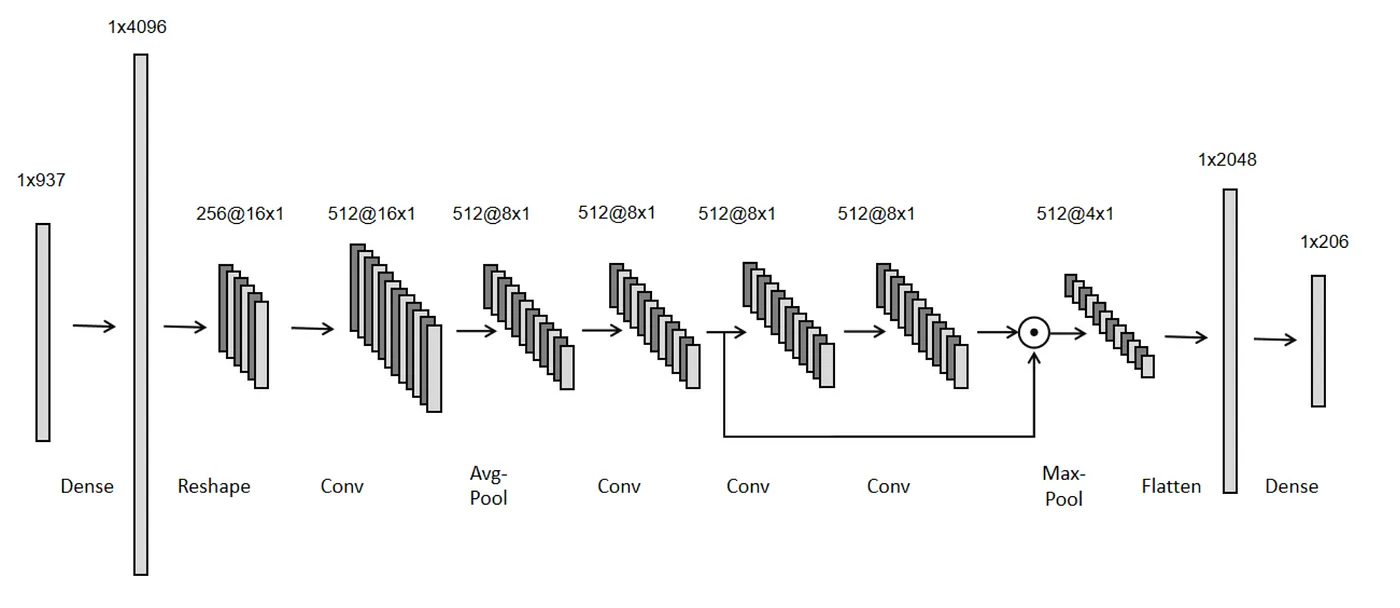
\includegraphics[width=1\textwidth]{figures/softOrdering1D.png}
    \caption{Soft-ordering with 1D convolutional architecture.}
    \label{fig:softOrdering1D}
\end{figure}

The process of reducing the error consisted of two stages. 

\begin{enumerate}
    \item Adapting the proposed architecture to the Kaggle data using tensorflow.
    \item Modifying the initial version to incorporate techniques that address issues present in the proposed dataset.
\end{enumerate}

\subsubsection{Adapting the proposed architecture to the Kaggle data using tensorflow}

The implementation was carried out using Tensorflow, based on the proposed scheme. As shown in Listing~\ref{cod:reg_addition_desbalanced}, various components from the library were utilized, such as the different types of layers, activation functions required and different regularisation techniques. This elements contributed an improvement in prediction quality, as illustrated in Figure~\ref{fig:result_addtion_reg}. In this figure, the discrepance between the predicted and actual values of the \(LN\_IC_{50}\) variable is visible reduced, indicating lower dispersion and a more accurate model, as reflected in the metrics in Table~\ref{tab:model_metrics_add_desb}. In addition, it is very important to note that Figure~\ref{fig:result_addtion_reg} no longer shows the large error that when \(LN\_IC_{50}\) variable took high values.

\begin{table}[H]
    \centering
    \begin{tabular}{|c|c|}
    \hline
    \textbf{Metric} & \textbf{Value} \\
    \hline
    Loss & 0.098 \\
    RMSE & 0.504 \\
    \hline
    \end{tabular}
    \caption{Model performance metrics on the test set during the architecture adapting phase.}
    \label{tab:model_metrics_add_desb}
\end{table}

Despite improved results, it is still possible to achieve a better quality model.

To identify potential improvements to the model, it is important to analyze Figure~\ref{fig:train_addtion_reg}, which illustrates the evolution of the loss function during training. As shown in the figure, the model initially exhibits high error, which progressively decreases as it learns to adjust its parameters. At a certain point, the loss drops significantly, suggesting that the model begins to generalize key patterns relevant to the regression task. However, this improvement plateaus after a few iterations, with no further reduction in error.

Moreover, a considerable gap is observed between the training and validation errors, with the training loss being significantly lower. This discrepancy suggests that, although there is no clear indication of overfitting, the model performs considerably better on the training set than on the validation set. This implies that it may not be capturing generalizable patterns well enough to accurately predict unseen data. Reducing this gap could therefore help to achieve better results.

\begin{figure}[H]
    \centering
    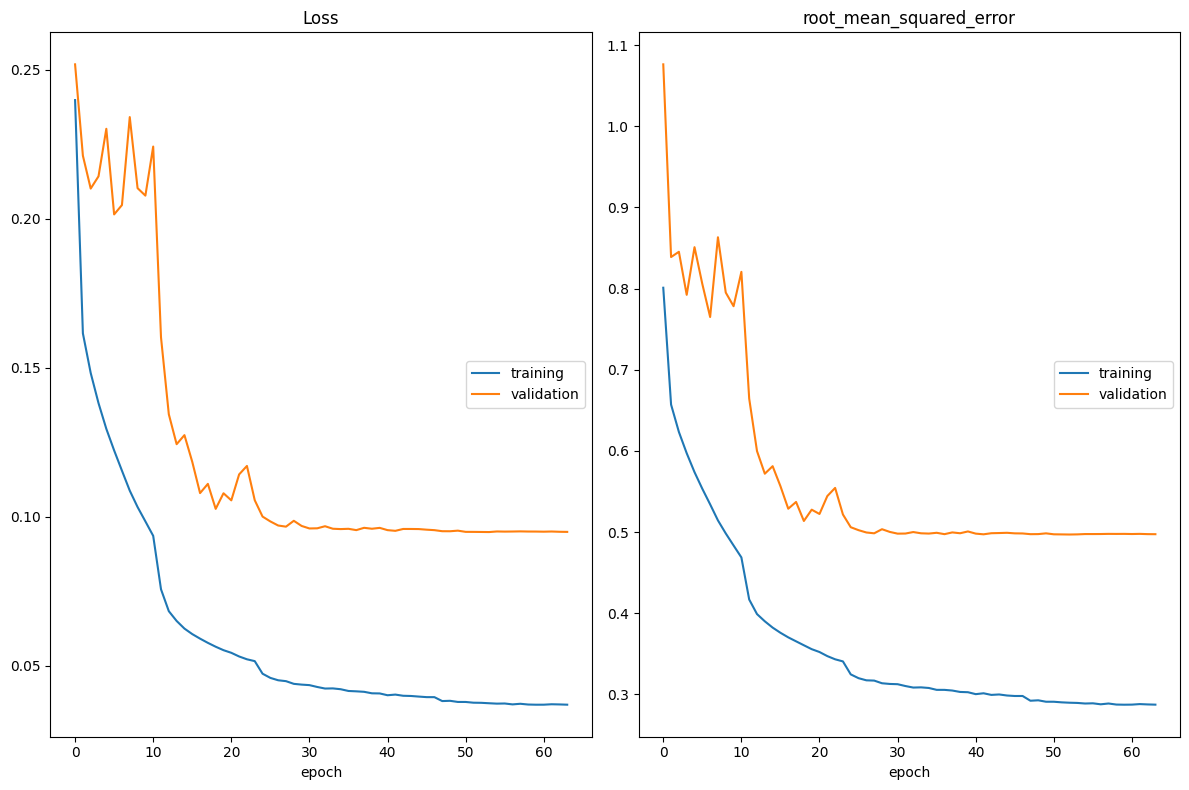
\includegraphics[width=1\textwidth]{figures/neural_net_regression_addition/train_logcosh_addition_desbalanced.png}
    \caption{Training a neural network using convolutional layers and addition as a bridge.}
    \label{fig:train_addtion_reg}
\end{figure}


\begin{figure}[H]
    \centering
    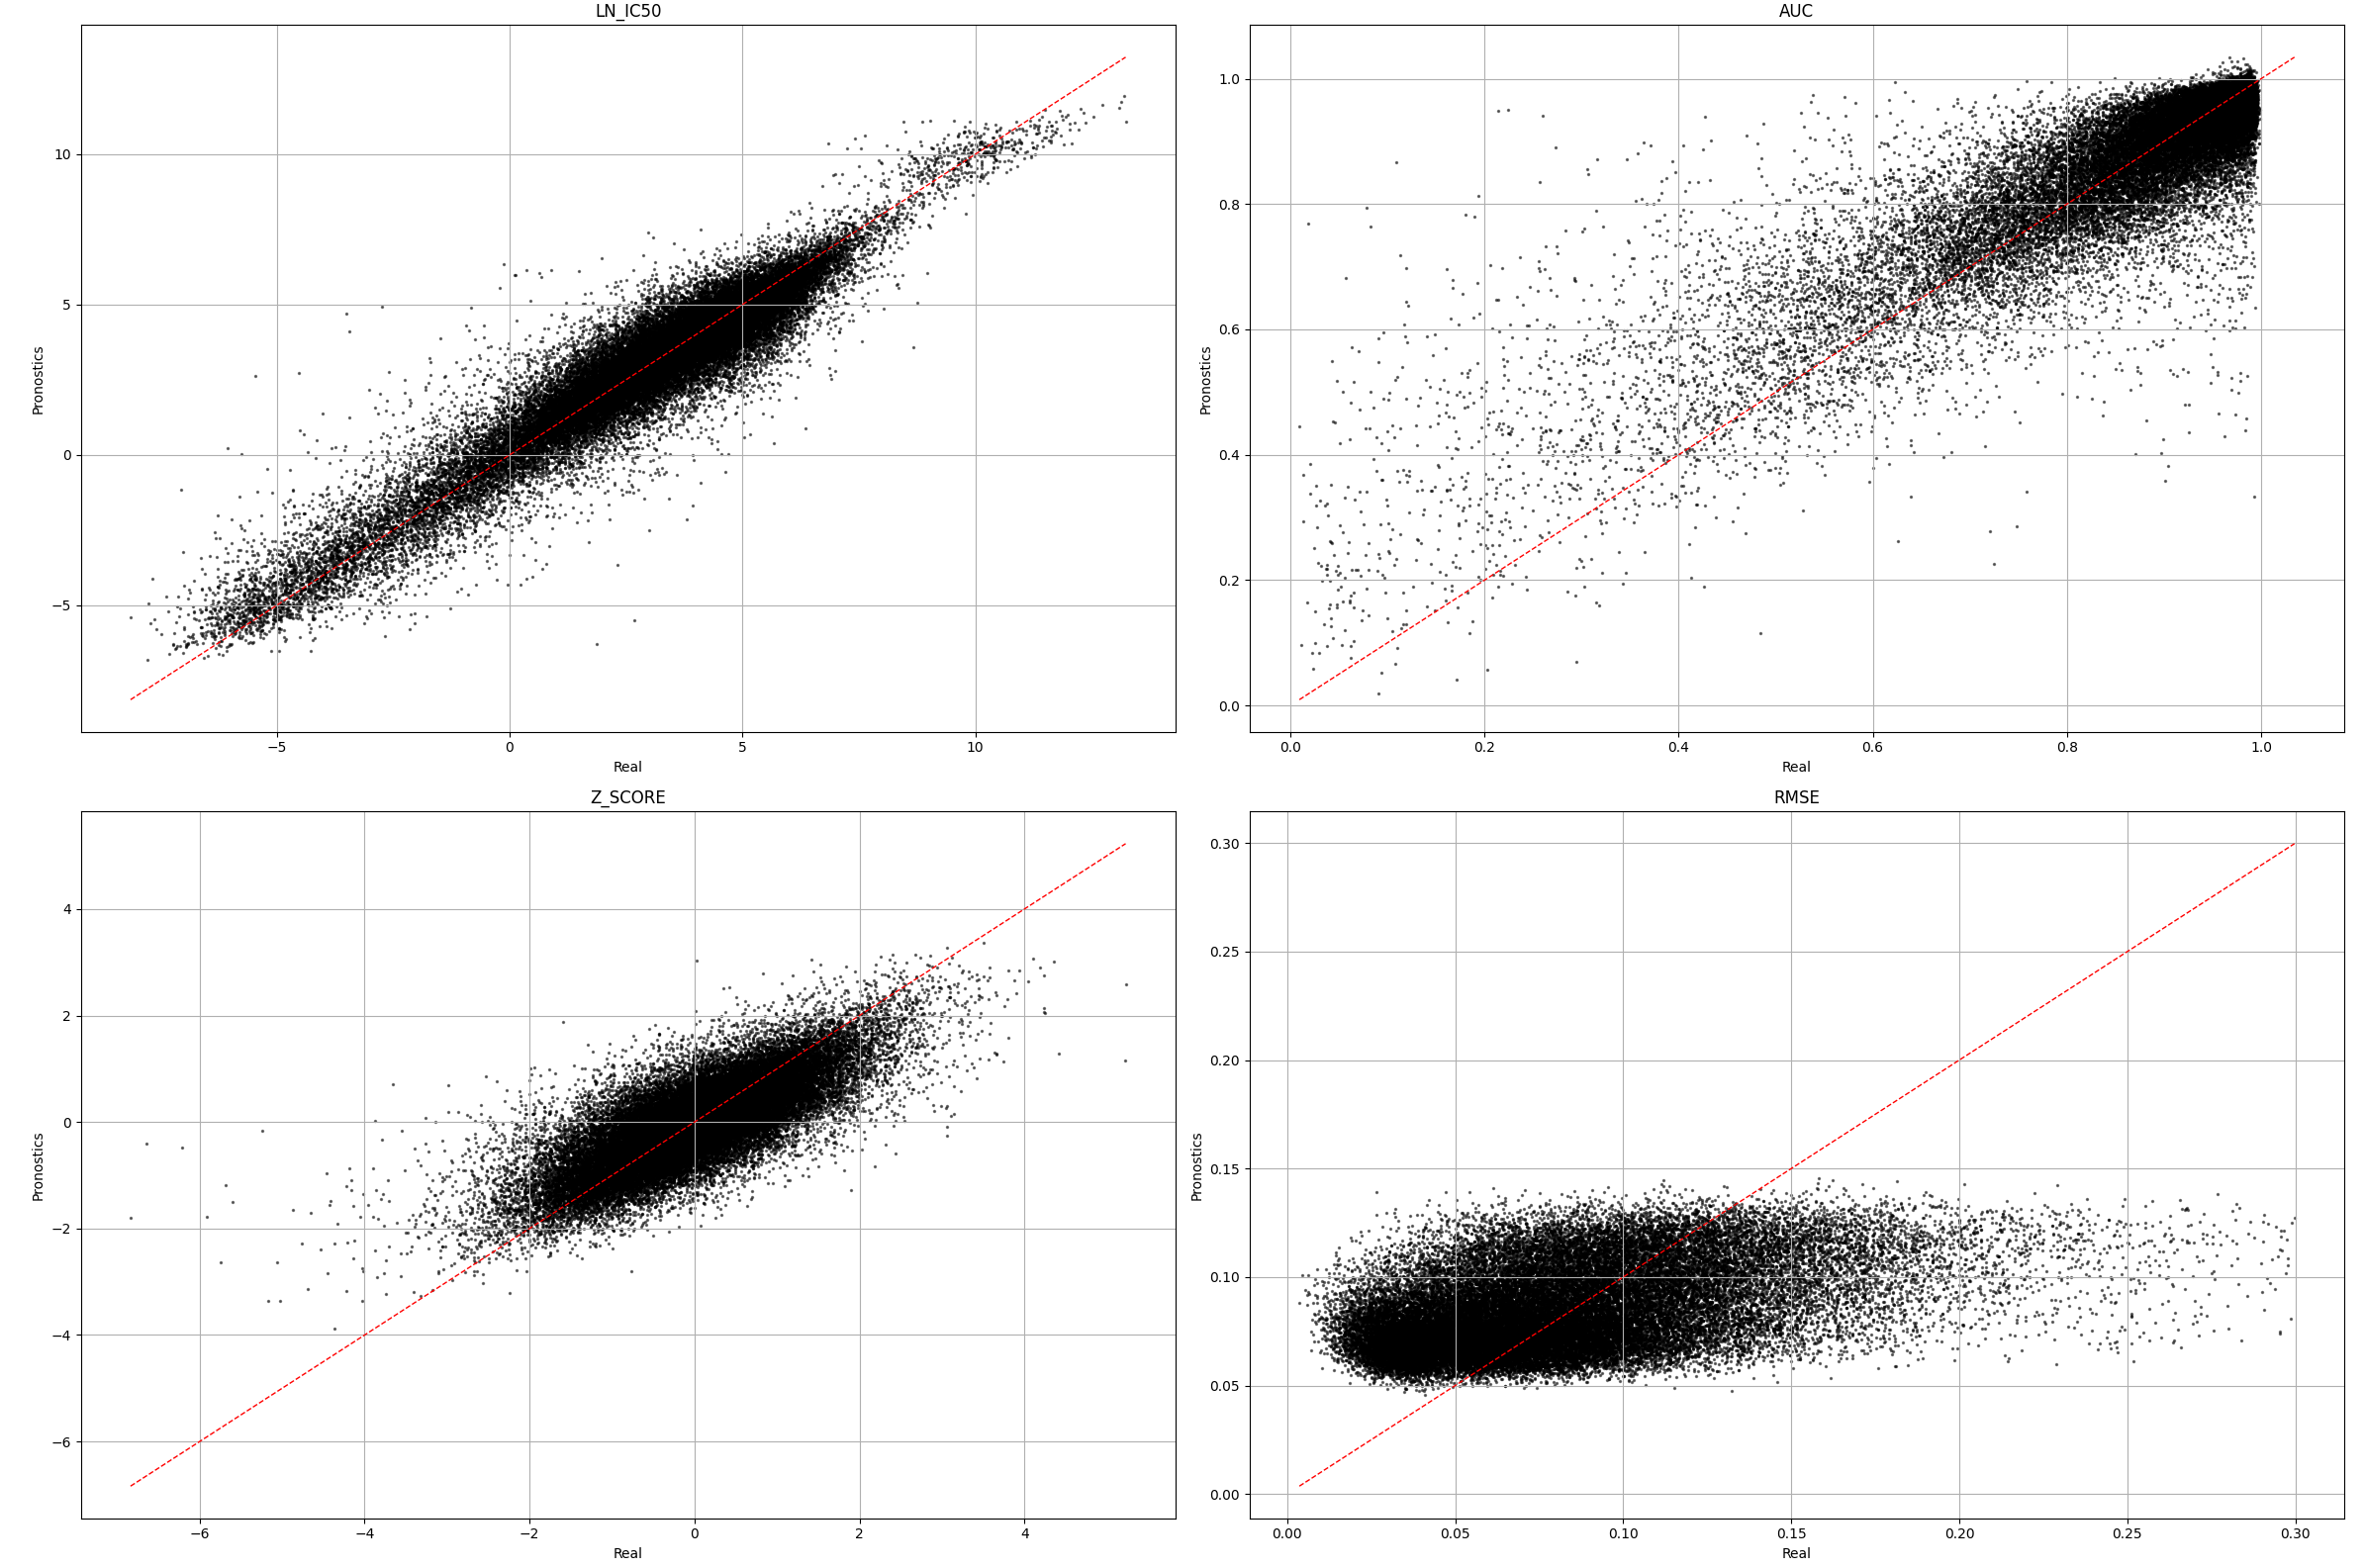
\includegraphics[width=1\textwidth]{figures/neural_net_regression_addition/output_neural_net_addition_desbalanced.png}
    \caption{Result of employing a neural network using convolutional layers and addition as a bridge.}
    \label{fig:result_addtion_reg}
\end{figure}

\subsubsection{Modifying the initial version to incorporate techniques that address issues present in the proposed dataset}

To mitigate overfitting, numerous experiments were conducted by increasing and varying different types of regularization techniques. However, the results remained largely unchanged, with only marginal improvements in error reduction. In contrast, experimenting with different activation functions led to more promising results. Initially, the functions suggested in the original paper were tested, but subsequently, other activation functions available in TensorFlow were explored. Among these, the SiLU function \cite{silu}, also known as Swish, proved particularly effective. It significantly reduced the gap between training and validation errors.

This improvement can be attributed to the characteristics of SiLU compared to ReLU and the specific nature of our dataset. SiLU is a smoother function with outputs close to zero, as illustrated in Figure~\ref{fig:compararisionSiluRelu}, making it more suitable in scenarios where small negative values may carry meaningful information. Unlike ReLU, which zeroes out all negative values, SiLU retains them with a small but non-zero output, allowing a more nuanced interpretation.

One of the main drawbacks of SiLU is its higher computational cost, as it requires computing a sigmoid function in addition to a multiplication operation. In contrast, ReLU simply computes the maximum between zero and the input value. The formula for SiLU is:

\[
\text{SiLU}(x) = x \cdot \sigma(x) = \frac{x}{1 + e^{-x}} \quad \text{where } \sigma(x) \text{ is the sigmoid function}
\]

\begin{figure}[H]
    \centering
    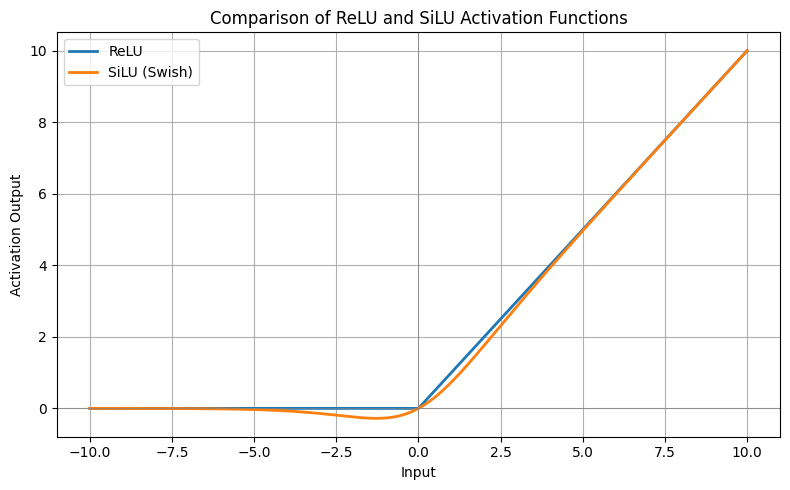
\includegraphics[width=1\textwidth]{figures/neural_net_regression_research/reluSilucomparison.png}
    \caption{ Comparision between SiLU and ReLU. In this picture it is observed the differeces between them around zero.}
    \label{fig:compararisionSiluRelu}
\end{figure}

On this basis, the implementation, shown in Listing~\ref{cod:reg_addition_balanced}, was carried out again, adjusting some of the hyperparameters related to the regularization and the number of layers. As a result of these modifications, the difference between the train and valiadation was reduced, showing a narrower gap, as is ilustrate by Figure~\ref{fig:train_addtion_reg_balanced}.

\begin{figure}[H]
    \centering
    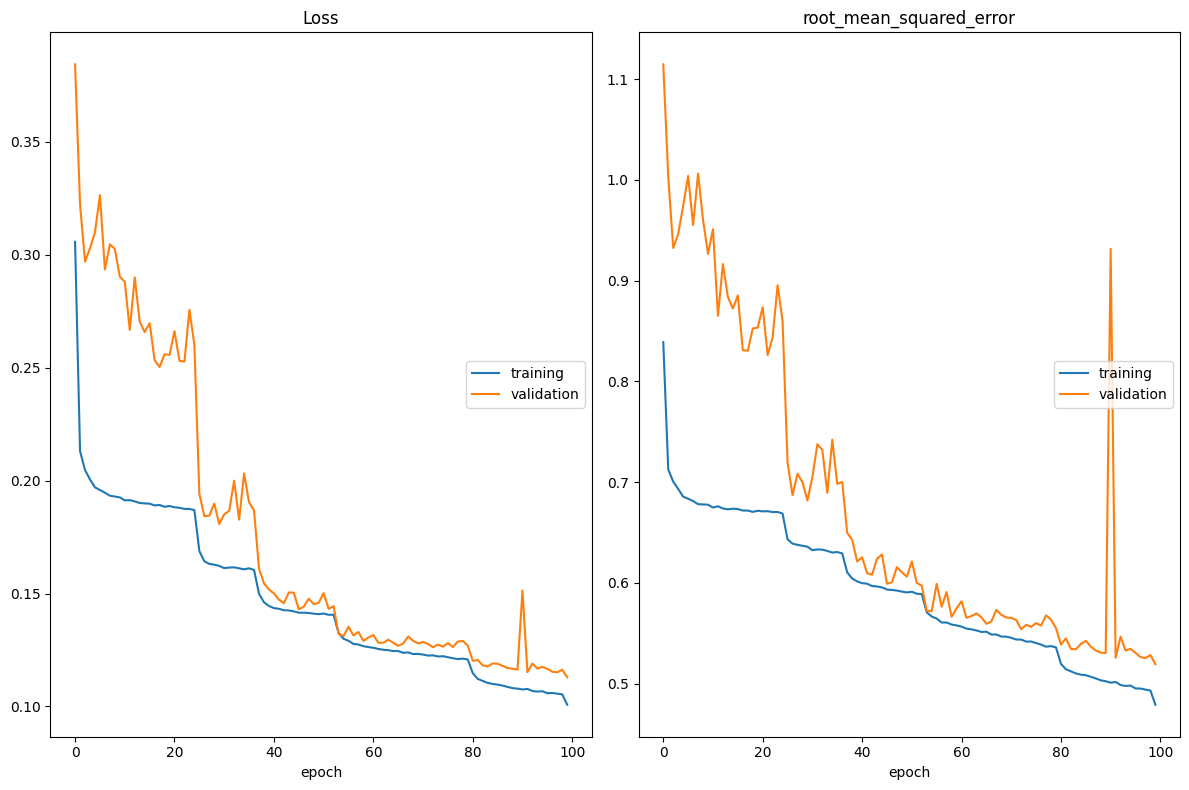
\includegraphics[width=1\textwidth]{figures/neural_net_regression_addition/train_logcosh_addition_balanced.png}
    \caption{Training a neural network using convolutional layers and addition as a bridge, increasing the regularization and using SiLU as activation function.}
    \label{fig:train_addtion_reg_balanced}
\end{figure}

\begin{table}[H]
    \centering
    \begin{tabular}{|c|c|}
    \hline
    \textbf{Metric} & \textbf{Value} \\
    \hline
    MSE & 0.270 \\
    RMSE & 0.520 \\
    MAE & 0.257 \\
    R\textsuperscript{2} & 0.685 \\
    \hline
    \end{tabular}
    \caption{Performance metrics on the test set after applying the SiLU activation function.}
    \label{tab:metrics_silu}
\end{table}

\begin{figure}[H]
    \centering
    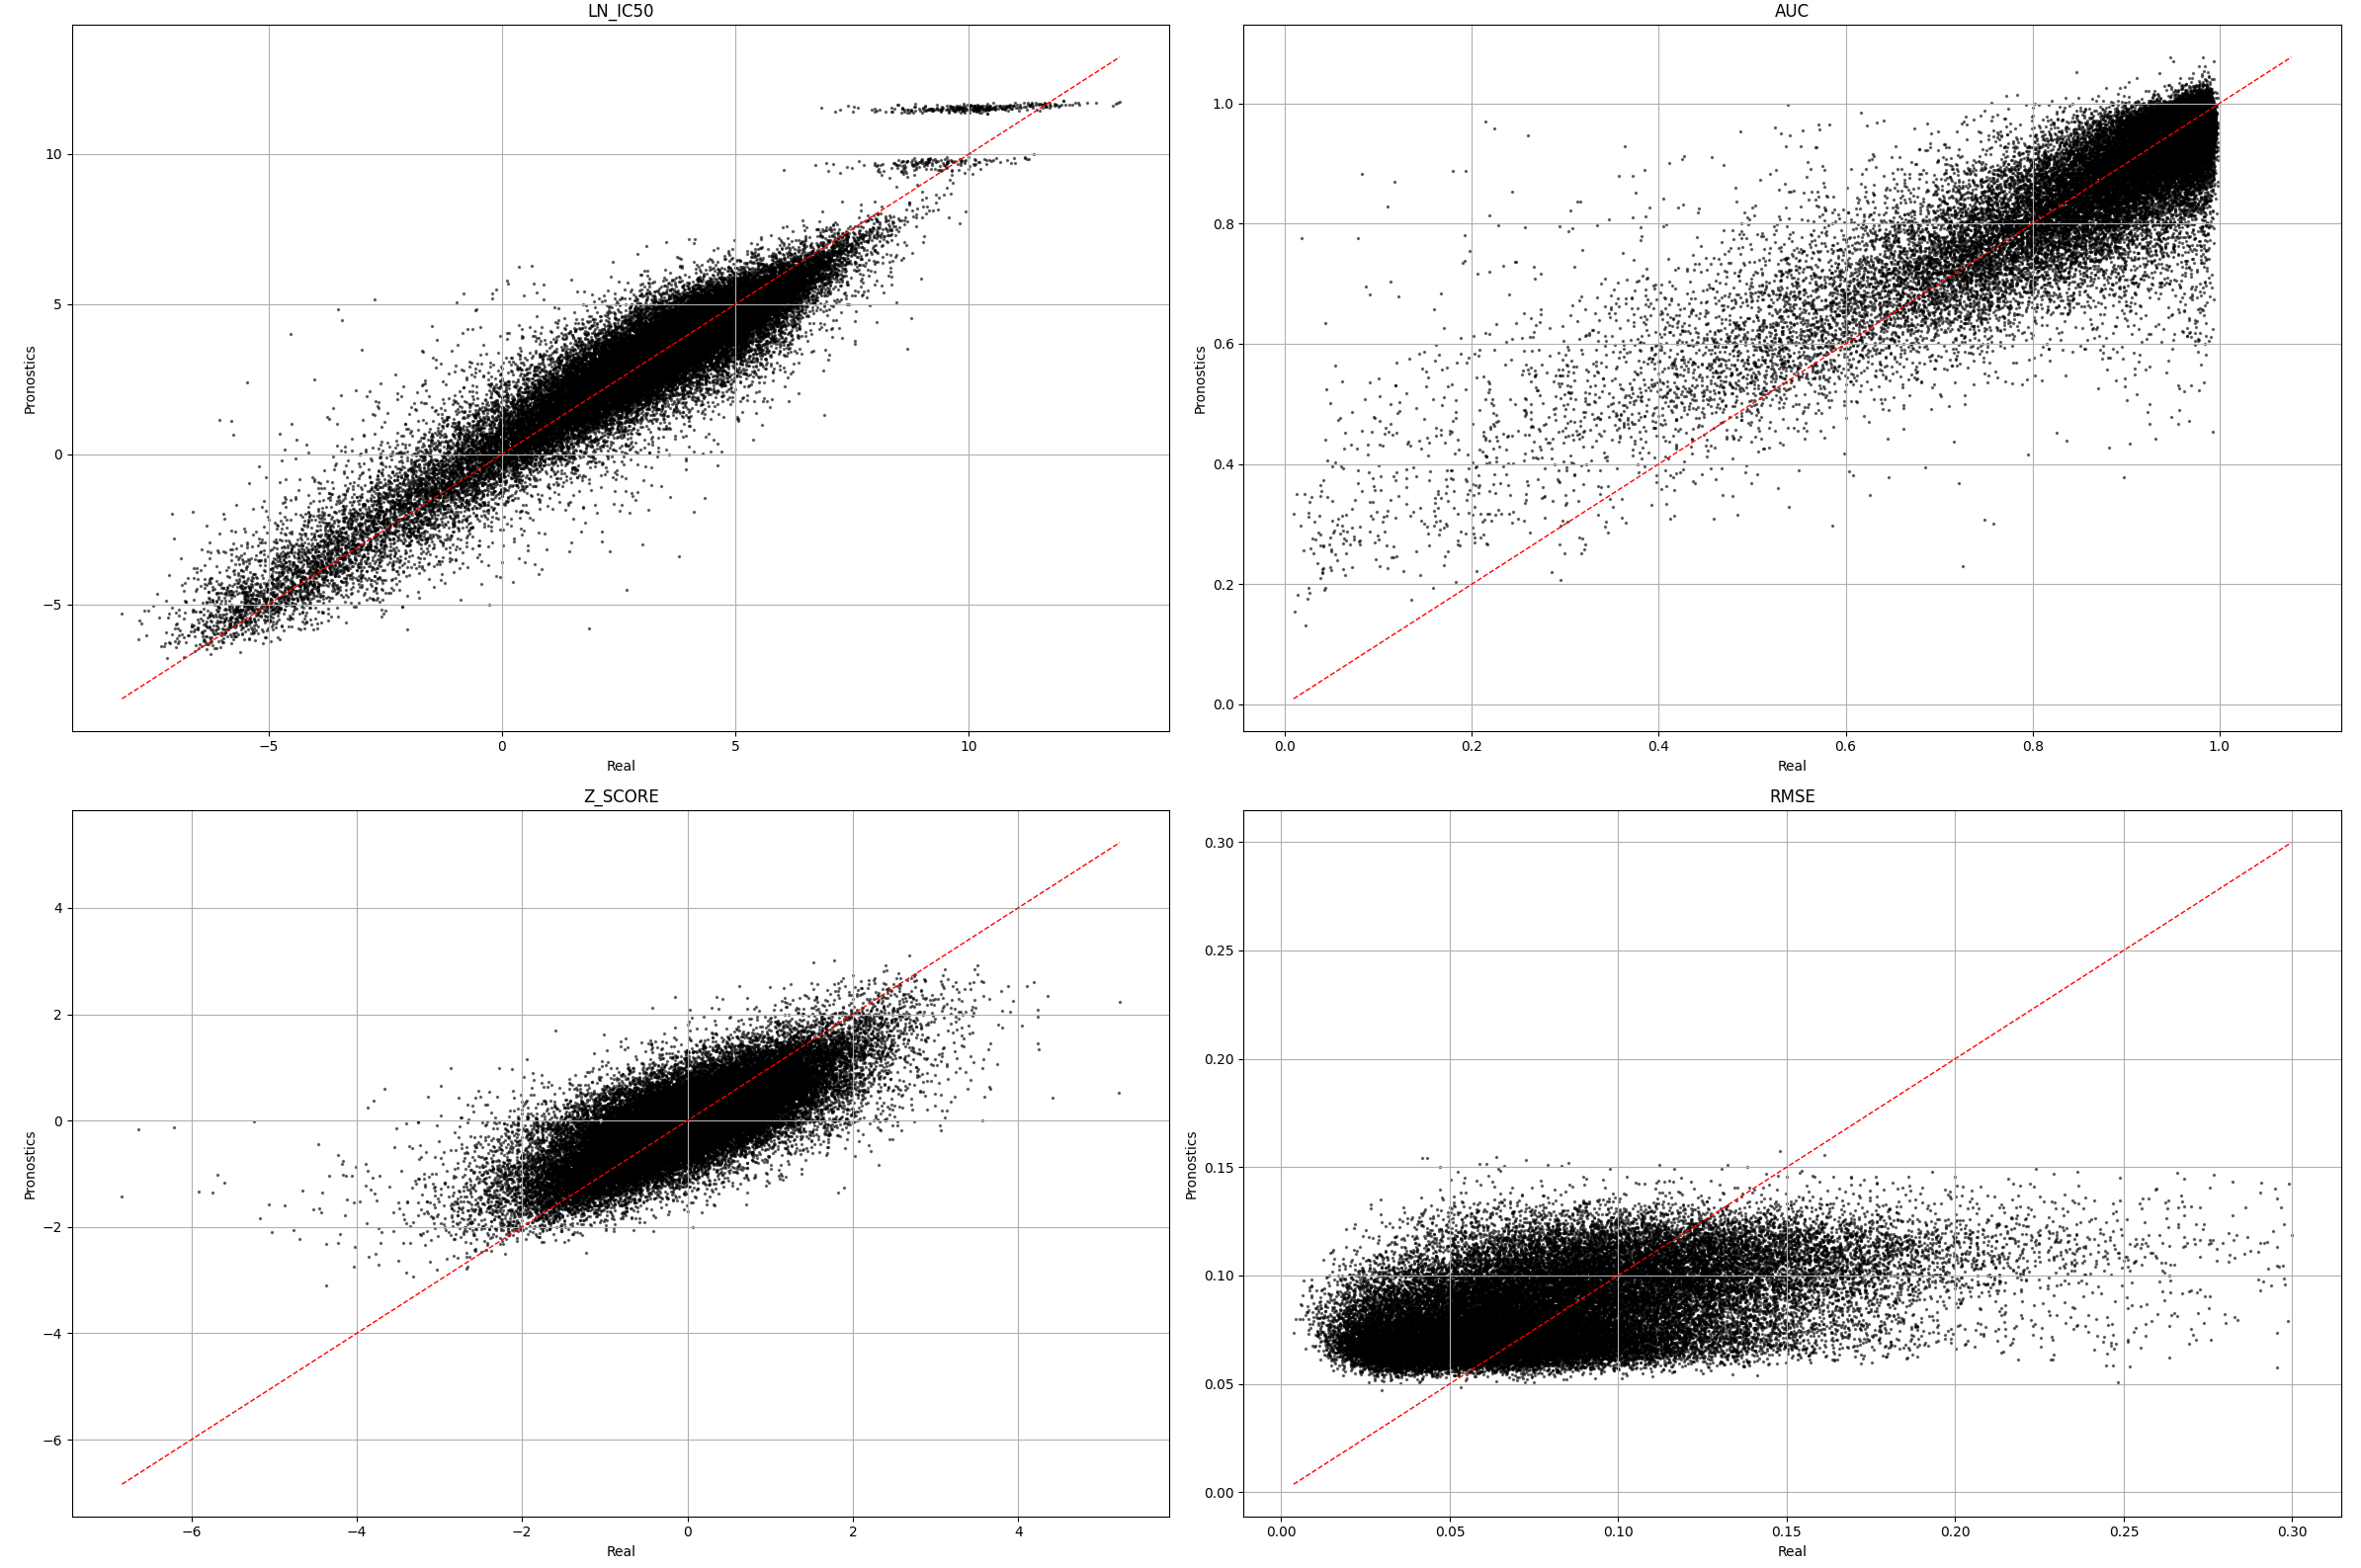
\includegraphics[width=1\textwidth]{figures/neural_net_regression_addition/output_neural_net_addition_balanced.png}
    \caption{Result of employing a neural network using convolutional layers and addition as a bridge, increasing the regularization and using SiLU as activation function.}
    \label{fig:result_addtion_reg_balanced}
\end{figure}

After this improvement in training stage, another challenge was found. The error was increased, as can be seen in Figure~\ref{fig:result_addtion_reg_balanced}. Not only did the spread for the predictions for the \(LN\_IC_{50}\) variable become wider, but the model also performed worse when predicting high values in comparation with the previous version.

This prompted a new line of research focused on improving the prediction results, trying to avoid increase the gap between training and validation again. In this situation, the best alternative was to investigate how to improve an architecture based on convolutions for other types of problems, in particular those related to images, since this is where most research has been done. 

\subsubsection{Custom architecture}

After extensive research, it became clear that one way to cancel out neurons or drastically reduce their impact was through multiplication \cite{contextgatedconvolution, gatedscnngatedshapecnns}. Thus, thinking about how to adapt this mechanism to the current architecture came to the fore, as it could be the answer to the problem. If possible, the model could learn to discriminate between points that are of no interest, providing better results.

Motivated by this idea, various ways of modifying the architecture to introduce multiplication were considered, two of which stood out:

\begin{itemize}
    \item Perform the addition as planned in the original model  and then apply the multiplication. This adaptation caused problems in the performance of the model.
    \item Replace the addition with multiplication, thereby reducing the freedom of the model compared to the previous approach. This design acts as an attention-like filter, helping the model distinguish important from irrelevant patterns. 
\end{itemize}


After observing the results of both proof-of-concept tests, the decision was clear. The implementation focused on replacing one operation with the other. As a result of this modification, the model provides better results in the test set, as evidenced by the metrics presented in Table~\ref{tab:metrics_multiplicative_gating}. Additionally, Figure~\ref{fig:result_multiply_reg_balanced} shows predictions with a lower degree of dispersion than any previous representation. This marks a key a milestone in the research, since the model achieved at this point is capable of estimating the value of the \(LN\_IC_{50}\) variable with great precision. Notably, it maintains its performance even for data points with exceptionally high \(LN\_IC_{50}\) values, not as it happened in Figure~\ref{fig:result_addtion_reg_balanced}. 

Given the absence of significant discrepancies between validation and test errors during training, this model is a strong candidate for applying explainability techniques. The insights derived could offer meaningful contributions to oncological research aimed at advancing cancer treatment

\begin{table}[H]
    \centering
    \begin{tabular}{|c|c|}
    \hline
    \textbf{Metric} & \textbf{Value} \\
    \hline
    MSE & 0.240 \\
    RMSE & 0.490 \\
    MAE & 0.242 \\
    R\textsuperscript{2} & 0.694 \\
    \hline
    \end{tabular}
    \caption{Performance metrics on the test set after incorporating the multiplicative gating mechanism.}
    \label{tab:metrics_multiplicative_gating}
\end{table}

\begin{figure}[H]
    \centering
    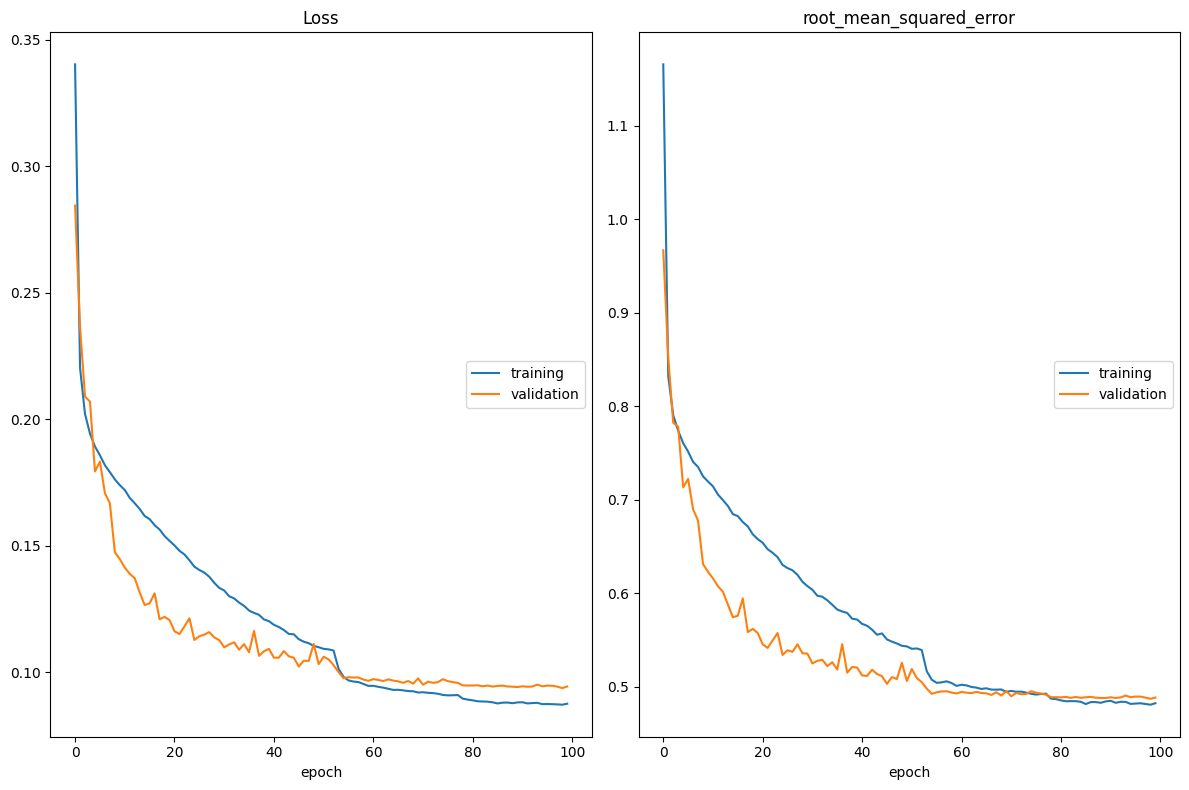
\includegraphics[width=1\textwidth]{figures/neural_net_regression_multiplication/train_logcosh_multiplication_silu.png}
    \caption{Training a neural network using convolutional layers and multiplication as a bridge.}
    \label{fig:train_multiply_reg_balanced}
\end{figure}

\begin{figure}[H]
    \centering
    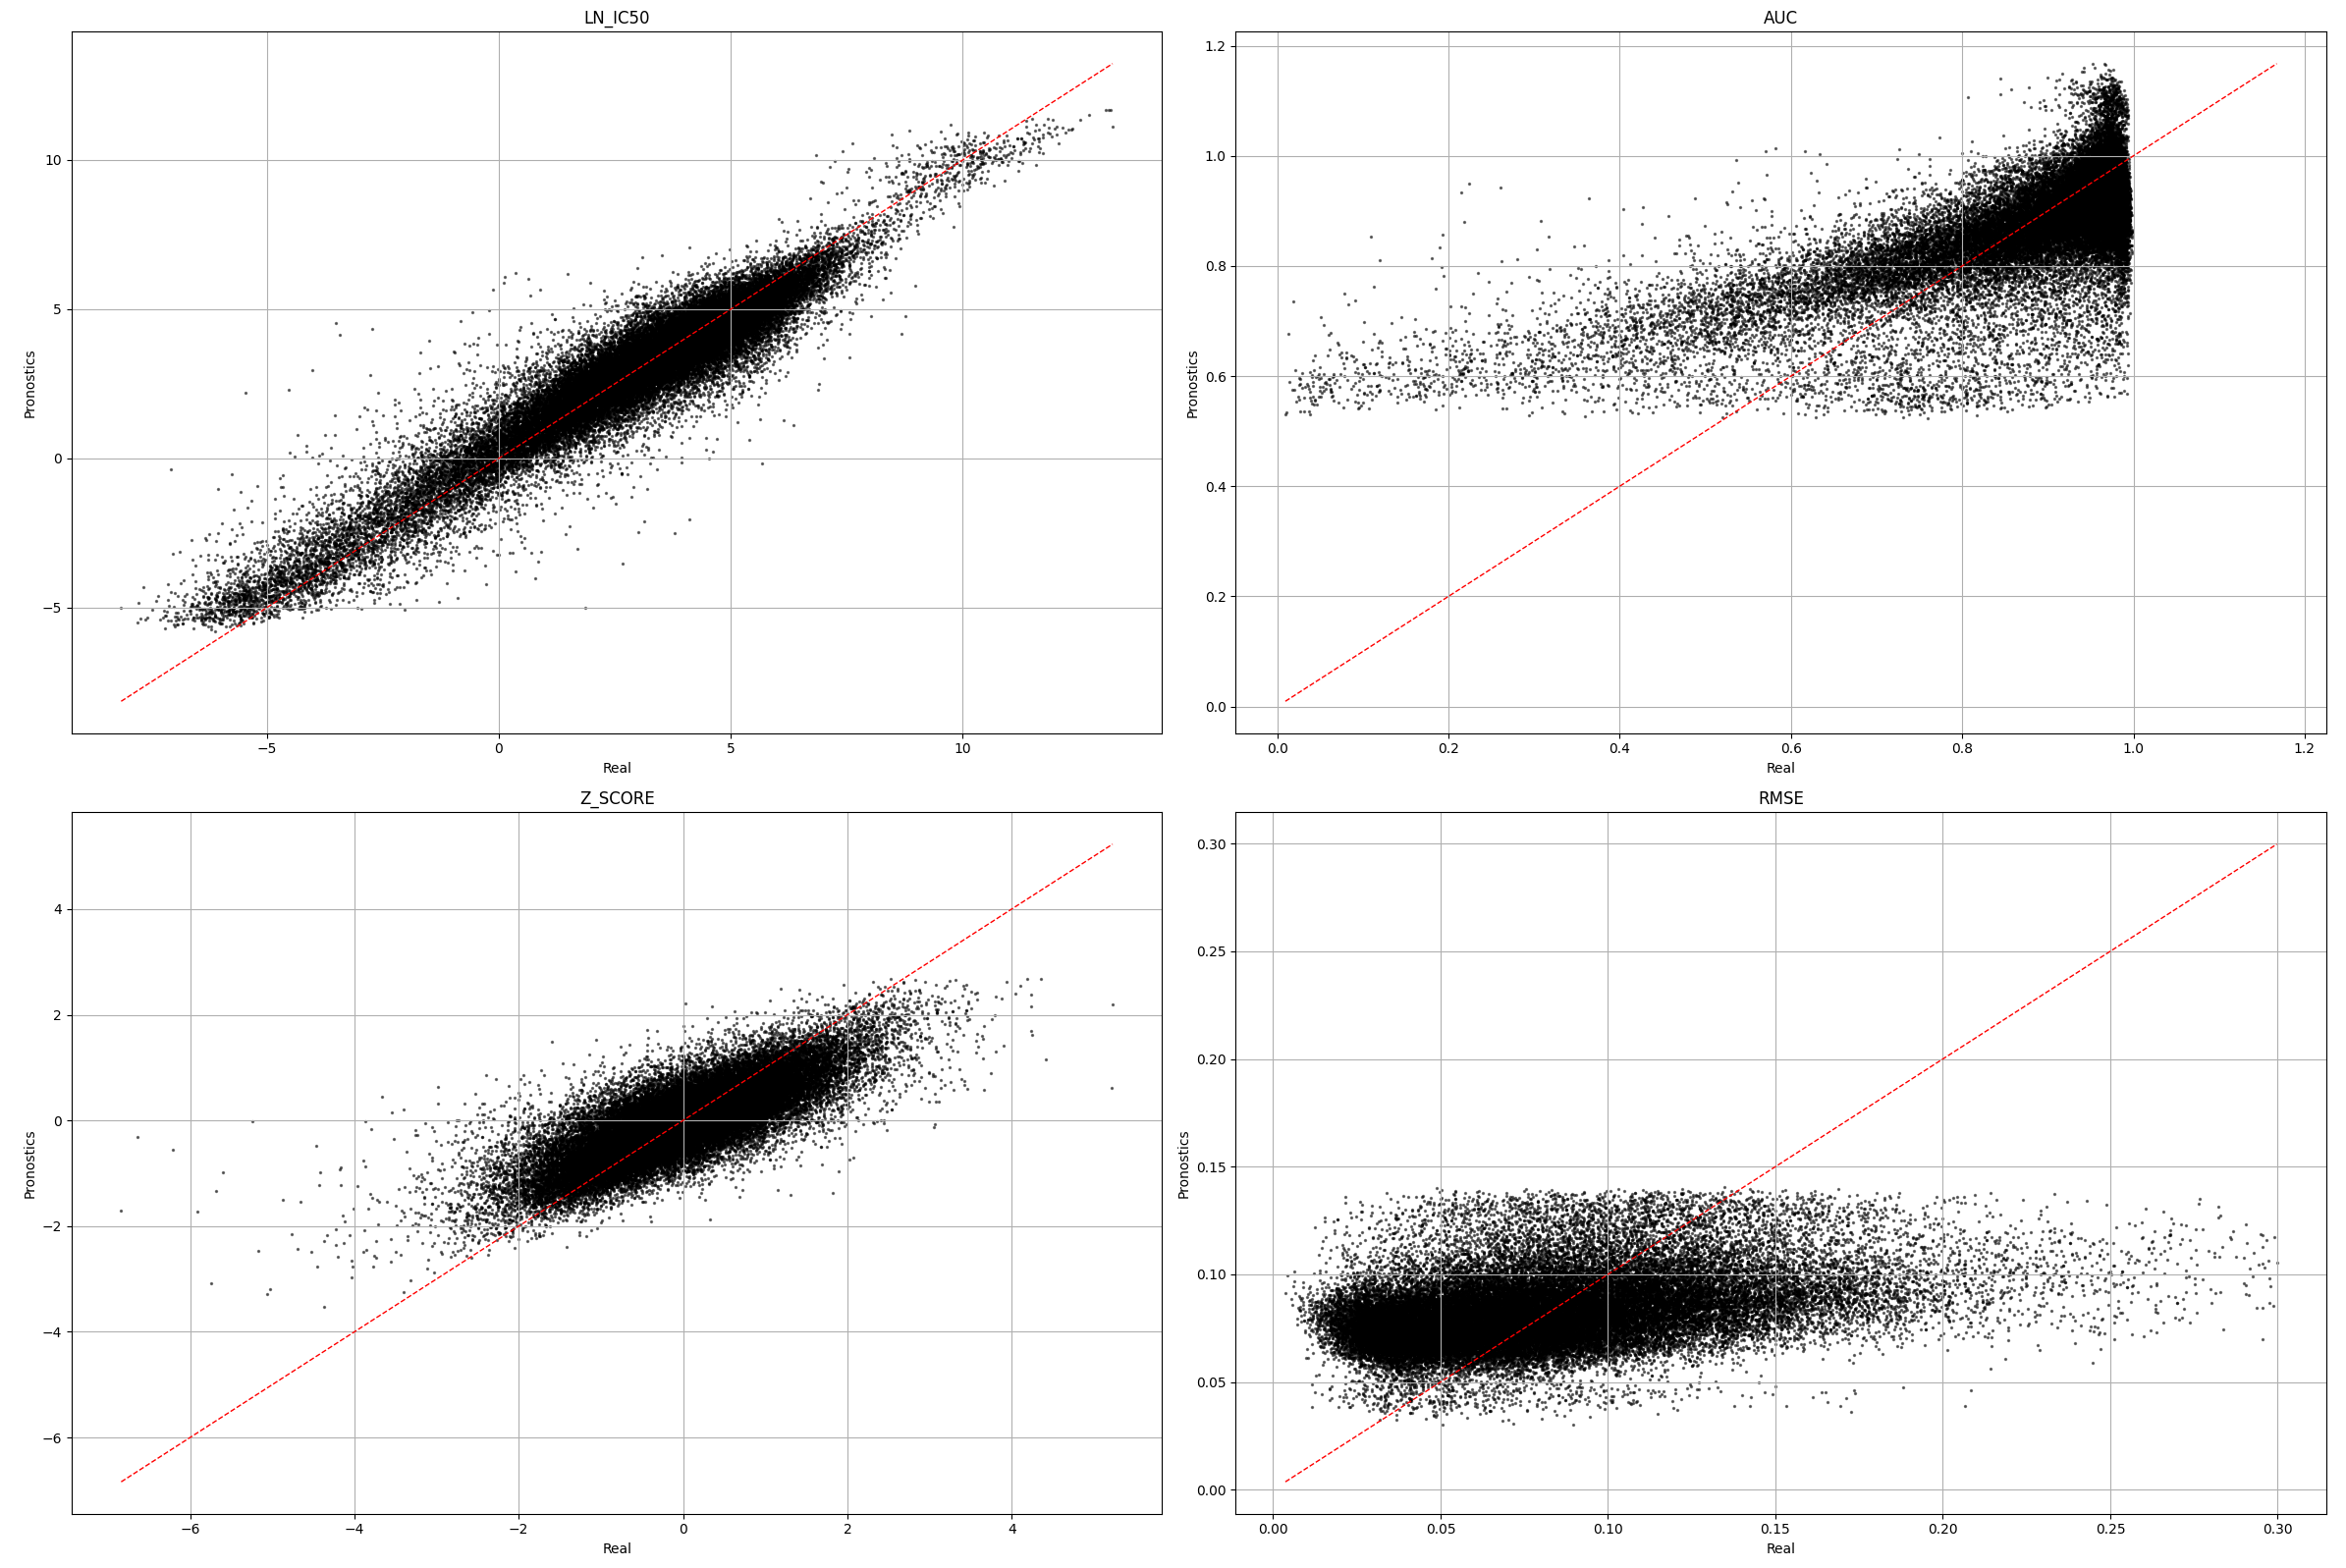
\includegraphics[width=1\textwidth]{figures/neural_net_regression_multiplication/output_neural_net_multiplication_silu.png}
    \caption{Result of employing a neural network using convolutional layers and multiplication as a bridge.}
    \label{fig:result_multiply_reg_balanced}
\end{figure}


\subsection{Application of XGBoost Regression Trees to our problem}

Currently, much of the research being conducted uses neural networks, but one should never assume that one type of architecture is always optimal for all cases. For this reason, this study includes some experiments with tree-based algorithms as well, in order to increase the knowledge of the problem. As stated at the beginning of this chapter, the chosen algorithm is XGBoost because it has shown very good results in several articles \cite{zheng2024advancedpaymentsecuritysystemxgboost, Computer-aided-boosting}.

Tree-based models have a major disadvantage compared to networks, they are typically poor at extrapolation, meaning they struggle to predict values outside the range observed during training. But even so, they are characterised by their great robustness and, due to their nature, they allow the elimination of variables without adding cost, since it is the algorithm itself that determines the features that are relevant to achieve the objective.

To enable a fair comparison between models, an XGBoost model was trained using the same dataset that was previously used for the neural networks. This approach ensures that both models are evaluated under identical conditions, allowing us to assess their respective performance accurately.

Several training sessions were performed using the XGBoost library available for Python, through which the following results were obtained:

\begin{table}[H]
    \centering
    \begin{tabular}{|c|c|}
    \hline
    \textbf{Metric} & \textbf{Value} \\
    \hline
    MSE & 1.253 \\
    RMSE & 1.119 \\
    R\textsuperscript{2} & 0.842 \\
    \hline
    \end{tabular}
    \caption{Performance metrics of the evaluated model on test set using XGBoost.}
    \label{tab:model_performance_xgboost}
\end{table}

\begin{figure}[H]
    \centering
    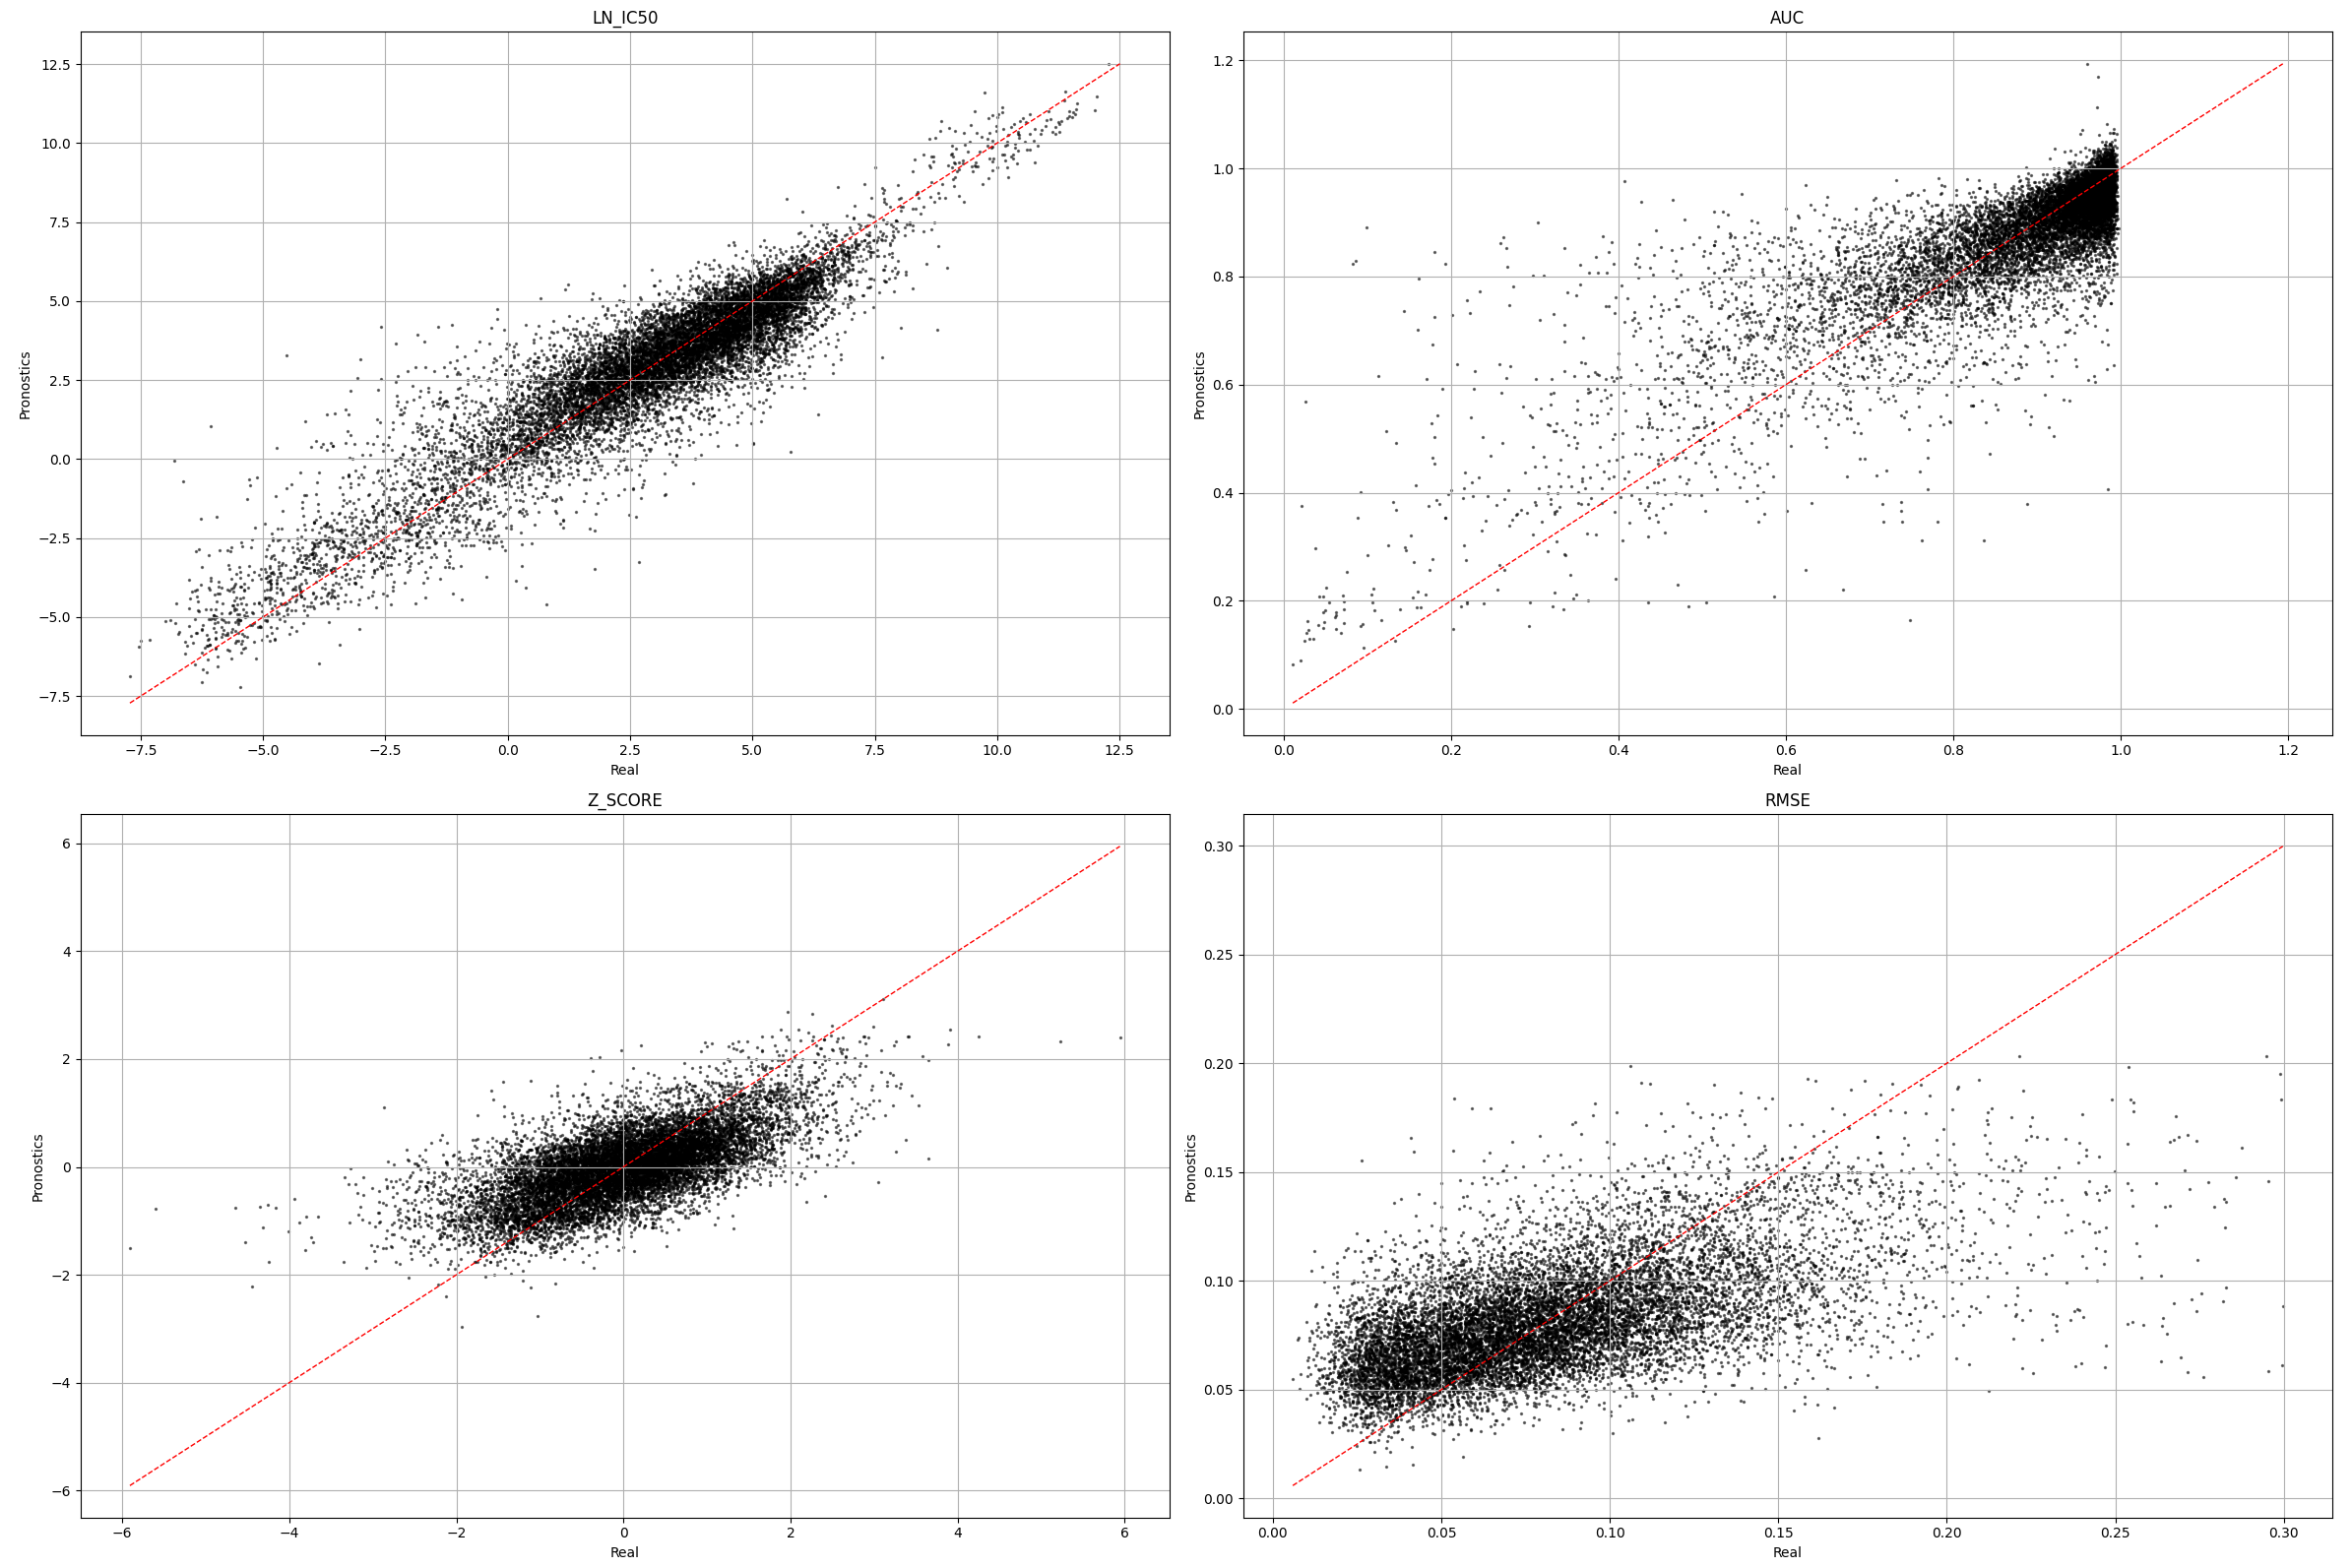
\includegraphics[width=1\textwidth]{figures/xgboost_reg/xgboost_reg_all_one_hot.png}
    \caption{Results of XGBoost with target variables encoded using one-hot.}
    \label{fig:train_xgboost_reg}
\end{figure}

Examining the performance of the model trained with XGBoost, as shown in Figure~\ref{fig:train_xgboost_reg} and Table~\ref{tab:model_performance_xgboost}, a decline in accuracy is observed compared to the neural network-based models. Specifically, the results suggest that XGBoost yields poorer predictions for the \(LN\_IC_{50}\) variable, while slightly improving the error for the remaining target variables. In other words, it increases the error in \(LN\_IC_{50}\) while reducing it for the others. However, this behavior is not desirable, as \(LN\_IC_{50}\) is the primary variable of interest. The other target variables serve merely as auxiliary signals to support the model during training and help improve its performance on the main target.

To improve the results, several hyperparameter optimization algorithms were applied, including GridSearch \cite{scikit-learn-gridsearchcv} and RandomSearch \cite{scikit-learn-randomizedsearchcv}. However, due to the presence of numerous features encoded using one-hot encoding, executing these processes required substantial computational resources, particularly in terms of RAM. This limitation posed a challenge, as such resources were not readily available. Various alternatives were evaluated to address this issue. Ultimately, ordinal encoding \cite{scikit-learn-onehotencoder} was applied to the one-hot encoded variables. This approach significantly reduced the number of columns, enabling the execution of different methods aimed at identifying dispensable variables. Among the algorithms used for this purpose were RFE \cite{scikit-learn-rfe} and SelectFromModel \cite{scikit-learn-selectfrommodel}.

In order to narrow down the variables to be eliminated, both feature selection methods, SelectFromModel and RFE, were run and those that were common to the two subsets generated were chosen. In this way, it was possible to reduce the number of variables to only 8, from 20 that were initially generated. Subsequently, RandomSearch was applied to try to find a good combination of hyperparameters, which one can be seen in Table~\ref{tab:gbm_params}. 

After that, the model was trained again. Two training were executed, the fir, using the variables with the ordinal encoder, and the second training with one-hot coding. Unfortunately, both results were of lower quality than those offered by the neural networks, as can be seen in Table~\ref{tab:xgboost_metrics_reducted}, which shows an increase in error. The best-performing model among the tested configurations was the one using one-hot encoding. It achieved the following evaluation metrics:

\begin{table}[H]
    \centering
    \begin{tabular}{|c|c|}
    \hline
    \textbf{Metric} & \textbf{Value} \\
    \hline
    MSE & 1.318 \\
    RMSE & 1.148 \\
    MAE & 0.855 \\
    R\textsuperscript{2} & 0.827 \\
    \hline
    \end{tabular}
    \caption{Performance metrics of the XGBoost model using one-hot encoding after hyperparameter optimization and variable selection.}
    \label{tab:xgboost_metrics_reducted}
\end{table}

\begin{figure}[H]
    \centering
    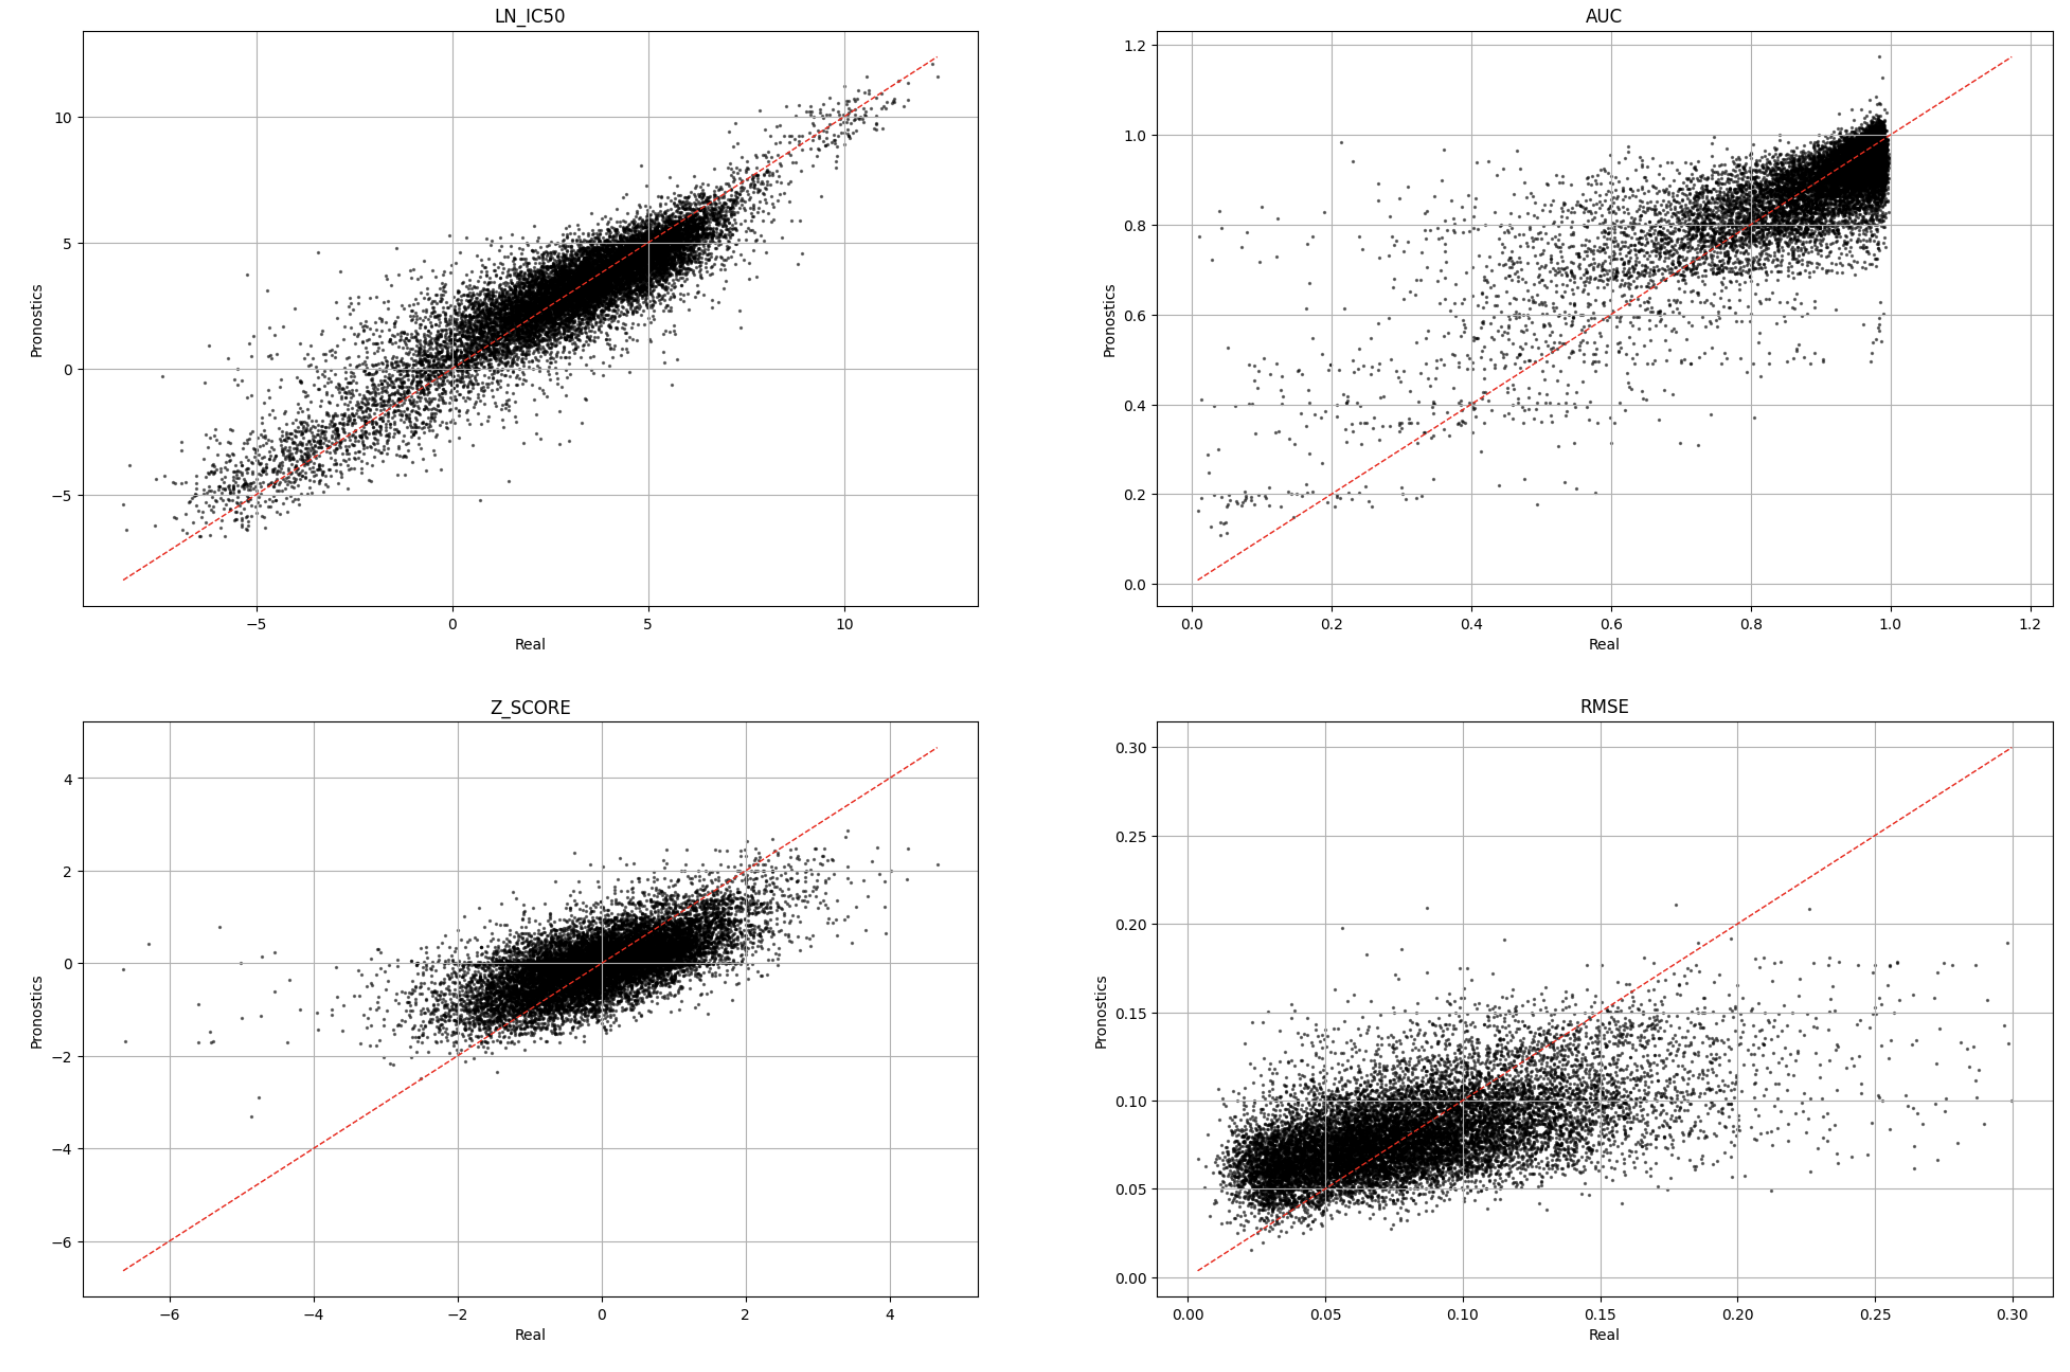
\includegraphics[width=1\textwidth]{figures/xgboost_reg/xgboost_optimized_reduced.png}
    \caption{Representation of predictions using XGBoost, together with feature reduction and hyperparameter optimisation.}
    \label{fig:xgboost_opt_red}
\end{figure}

\begin{table}[H]
    \centering
    \begin{tabular}{|c|c|}
    \hline
    \textbf{Parameter} & \textbf{Value} \\
    \hline
    \texttt{n\_estimators} & 869 \\
    \texttt{seed} & 123 \\
    \texttt{learning\_rate} & 0.028 \\
    \texttt{max\_depth} & 7 \\
    \texttt{reg\_alpha} & 0.040 \\
    \texttt{reg\_lambda} & 0.492 \\
    \texttt{max\_leaves} & 328 \\
    \hline
    \end{tabular}
    \caption{Hyperparameters of the gradient boosting model after applying hyperparameter optimization.}
    \label{tab:gbm_params}
\end{table}

\section{A classification problem}

The previous section has focused on continuous target variables, except for Drug Response, successfully developing a neural network-based regressor capable of predicting the \(LN\_IC_{50}\) variable with high accuracy, achieving an RMSE below 0.5. Building upon this strong foundation, the next step aims to bring the model closer to a real-world clinical application. To do this, the continuous \(LN\_IC_{50}\) variable is discretised into 25 equally spaced intervals, offering a practical approximation of dosage levels. 

This number of intervals has not been selected at random, but rather as a result of analysing the growth of entropy as a function of the number of divisions, particularly by observing the slope of this evolution. Maximising entropy allows to obtain a highly representative set, but an excessive number of divisions can introduce noise or redundancy. To avoid this problem, the slope of the entropy curve is analysed in order to identify an inflection point that indicates a balance between representativeness and stability. Thus, Figure~\ref{fig:intervalEntropy} illustrates the evolution of both entropy and the slope of its evolution. Based on this information, a division of 25 intervals is proposed, as this represents a midpoint between the slope and the increase in entropy. To carry out these operations, the code shown in Listing~\ref{cod:intervalEntropy} has been used.

\begin{figure}[H]
    \centering
    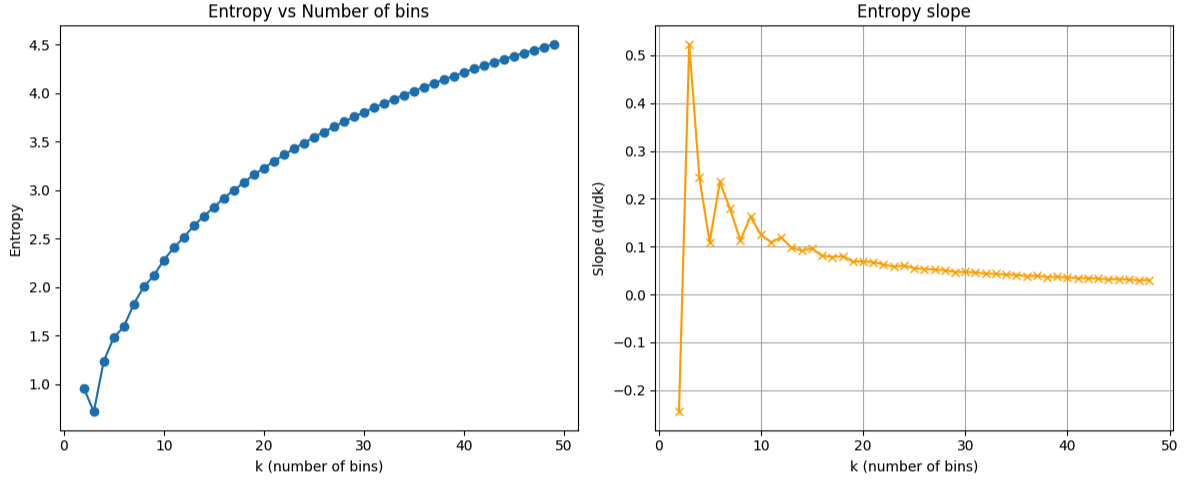
\includegraphics[width=1\textwidth]{figures/intervalEntropy.png}
    \caption{Representation of entropy evolution based on the number of bins.}
    \label{fig:intervalEntropy}
\end{figure}

The range in which the value of \(LN\_IC_{50}\) is found must be understood as the number of pills the patient should take. This idea makes a lot of sense, as getting closer to the concept of prescribing a certain number of pills allows to be somewhat more lax with the error made. For example, if two ibuprofens are taken instead of one, the negative effect is not appreciable. However, this is not the case when six are taken instead of one. Therefore, it can be inferred that making a slight error is not as serious as making a large one, an aspect that should certainly be considered when calculating the error.

Before any model is trained, the data will be visualized graphically to assess their separability, specifically, to determine whether the class ranges overlap in feature space or not. Since the dataset, after applying the ordinal encoder, contains more than 20 variables, direct representation is not feasible. Therefore, a dimensionality reduction process will be performed to project the data into 2D and 3D spaces, allowing for easier interpretation.

First, t-SNE \cite{cai2022theoreticalfoundationstsnevisualizing} will be used to perform the compression process. This algorithm is highly effective at capturing local relationships; that is, within a group, the relationships between data points can be accurately preserved. This will allow an assessment of whether points belonging to the same group are located close together in space. If they are not, it indicates higher data variance, which would make it more challenging for a model to correctly predict group membership.

For this purpose, the t-SNE method from scikit-learn \cite{scikit-learn-tsne} will be used. However, the algorithm is computationally expensive. To accelerate execution, the data obtained from the initial run will be saved using NumPy, so that subsequent executions can bypass the computational step. This process is illustrated in Listing~\ref{cod:tsne}.

\begin{figure}[H]
    \centering
    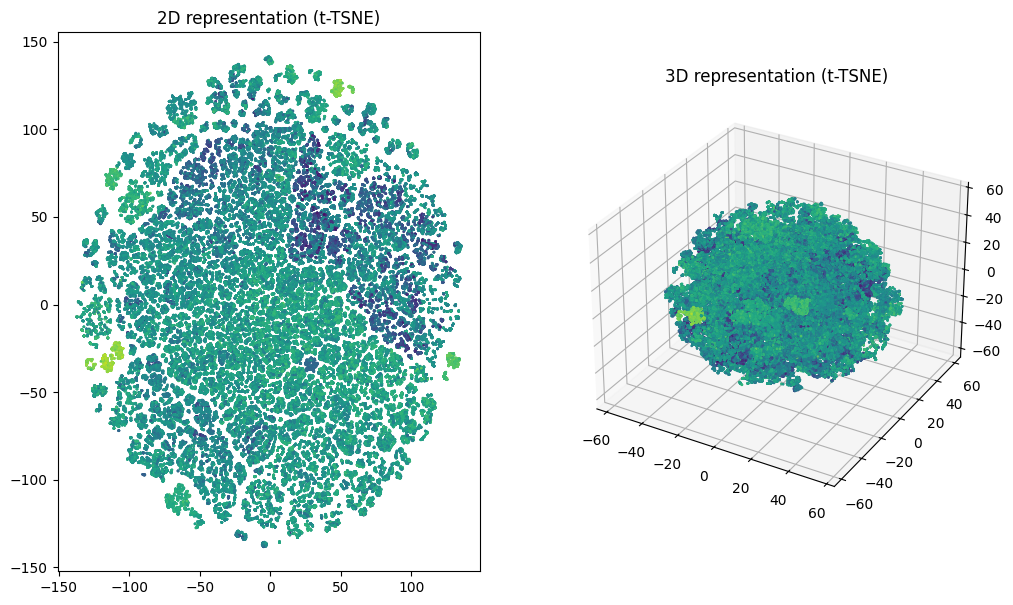
\includegraphics[width=1\textwidth]{figures/data_representation/tsne.png}
    \caption{Representation of the data by t-SNE, where it can be seen the separation between points of the same cluster.}
    \label{fig:tsne}
\end{figure}

As a result, the representation shown in Figure~\ref{fig:tsne} is obtained, in which the groups appear to be clearly distinguishable. However, a new question arises: although the clusters seem to be located close to one another in the plot, it is not certain whether this proximity reflects the true structure of the data, since t-SNE does not accurately capture global relationships, that is, the relationships between different groups.

To address this, UMAP \cite{mcinnes2020umapuniformmanifoldapproximation} will be used, as it is capable of preserving both local and global non-linear relationships. The implementation will be carried out using the umap-learn library \cite{umap-docs}, as demonstrated in Listing~\ref{cod:umap}. Similar to t-SNE, UMAP is computationally expensive; therefore, the same data-saving strategy will be applied to avoid repeated computations in future executions.

As a result, it can be observed in Figure~\ref{fig:umap} that the clusters are indeed well separated. Therefore, it can be assumed a priori that applying predictive models may yield good results.

\begin{figure}[H]
    \centering
    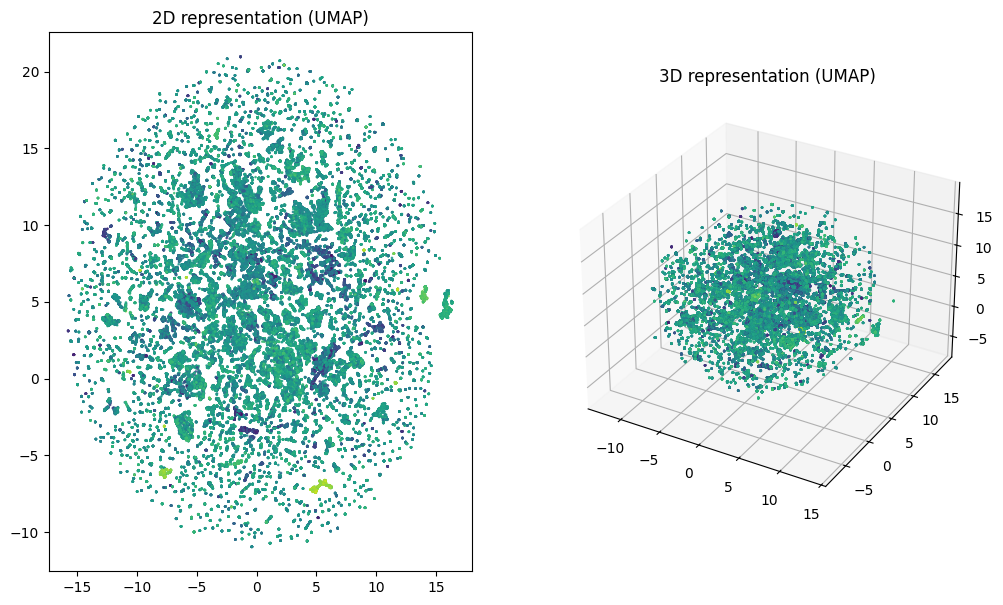
\includegraphics[width=1\textwidth]{figures/data_representation/umap.png}
    \caption{Representation of the data by UMAP, where it can be checked the distance between the different groups and their internal elements.}
    \label{fig:umap}
\end{figure}


\section{Discovering the correct group using Neural Networks}

The objective of this section is to estimate the number of doses required by a patient using a neural network. To accomplish this, the previously developed architecture must be adapted to effectively model the problem, beginning with the dataset that includes a discretized version of the target variable.

The process has been divided into three main stages:

\begin{enumerate}
    \item Adaptation of the existing architecture.
    \item Expansion paths
    \item Refinement of the loss function.
\end{enumerate}

\subsubsection{Adaptation of the existing architecture}

Building on the previously trained neural network model, the objective of this section is to obtain a new network capable of estimating the number of doses of a drug needed to treat a person. 
Acquiring a certain degree of intuition about how current architecture deals with classification issues is crucial to making changes that truly add value. Therefore, initially the changes will be subtle, i.e., only very specific sections of the architecture will be modified. In this way, after each modification that leads to an improvement in performance, it will be translated into the new goal to be achieved. To achieve this, it is necessary to modify both the loss function and the output layer of the model to make the predictions compatible with the classification.

Thus, the error function was replaced by categorical cross-entropy, which is one of the most used, with the aim of testing the model's accuracy. With regard to the model output, Softmax is the most recommended for this type of classification problem, as it provides a probability for each possible class. 

As there is more than one target variable, the network must have more than one output layer simultaneously, as can be seen in Listing~\ref{cod:class_net_v1}.

Once model training began, it successfully completed 100 epochs. The learning curves, shown in Figure~\ref{fig:train_class_net_v1}, reveal that the model achieves better performance on the validation set than on the training set, an uncommon but noteworthy behavior. However, despite this apparent advantage, the overall quality of the predictions remains limited, with accuracy values not exceeding 0.35, as can be seen in Table~\ref{tab:best_val_ln_ic50_metrics_net_class_v1}. This indicates that, although generalization may be occurring, the model still struggles to produce reliable predictions. Furthermore, depending on the progress of the training, the model would be able to improve if the number of available epochs were increased.

\begin{figure}[H]
    \centering
    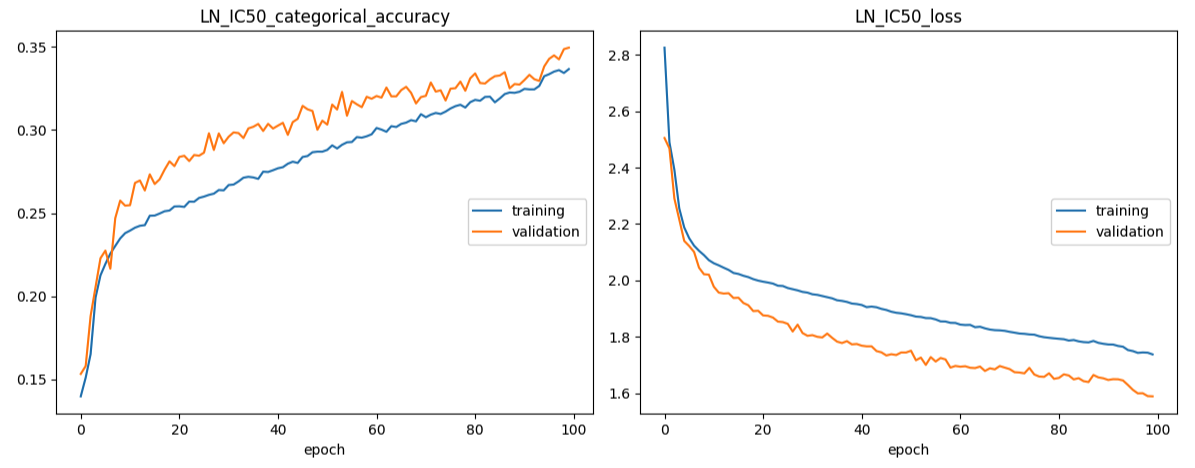
\includegraphics[width=1\textwidth]{figures/neural_net_classification/classification_mse_v1.png}
    \caption{Progress of model training after replacing the error function with cross-entropy and the output layer with a multi-class layer with softmax activation function. Better performance is observed in the validation set compared to the training set.}
    \label{fig:train_class_net_v1}
\end{figure}

\begin{table}[H]
    \centering
    \begin{tabular}{|l|c|}
    \hline
    \textbf{Validation Metric} & \textbf{Best Value} \\
    \hline
    LN\_IC50\_Categorical\_Accuracy & 0.349 \\
    LN\_IC50\_Loss & 2.505 \\
    \hline
    \end{tabular}
    \caption{Best validation results for LN\_IC50 metrics.}
    \label{tab:best_val_ln_ic50_metrics_net_class_v1}
\end{table}

\subsubsection{Expansion paths}

Refining the architecture so that the model is able to correctly capture the patterns present in the dataset is the next step towards achieving better results. Thus, the architecture currently proposed to act as a classifier has one main weakness: the error function. This is because it is unable to adjust to unbalanced data, for this reason it will be replaced by categorical focal cross-entropy. Depending on which one yields the most promising results, one or the other will be selected to form part of a customised function that takes into account the importance of large errors.

Additionally, giving greater relevance to the \(LN\_IC_{50}\) variable will help the model focus its efforts on correctly predicting this output. Without neglecting the extra knowledge provided by the others, thus serving as a support.

\subsubsection{Expansion paths: Loss function}

Among the loss functions suitable for classification tasks involving imbalanced classes, categorical focal cross-entropy is particularly worth considering. As an extension of the standard categorical cross-entropy, it introduces mechanisms specifically designed to mitigate the effects of class imbalance by emphasizing harder-to-classify examples. Applying this loss function can offer a useful indication of whether the class imbalance is significantly influencing model performance. 

The formula of this function is:

\[
\text{FL}(y, \hat{y}) = -\sum_{i=1}^{C} \alpha_i \, y_i \, (1 - \hat{y}_i)^\gamma \log(\hat{y}_i)
\]

\begin{itemize}
    \item \( C \): Total number of classes.
    \item \( y_i \): True label for class \( i \) (one-hot encoded).
    \item \( \hat{y}_i \): Predicted probability for class \( i \).
    \item \( \alpha_i \): Class weight (optional, used for class balancing).
    \item \( \gamma \): Focusing parameter (typically set to 2).
    \item \( (1 - \hat{y}_i)^\gamma \): Modulating factor that down-weights easy (high-confidence) examples.
\end{itemize}

Since the implementation is being carried out using the Tensorflow API, making this change is very simple. It only requires changing one line of text, as can be seen in Listing~\ref{cod:class_net_v2}.

\begin{figure}[H]
    \centering
    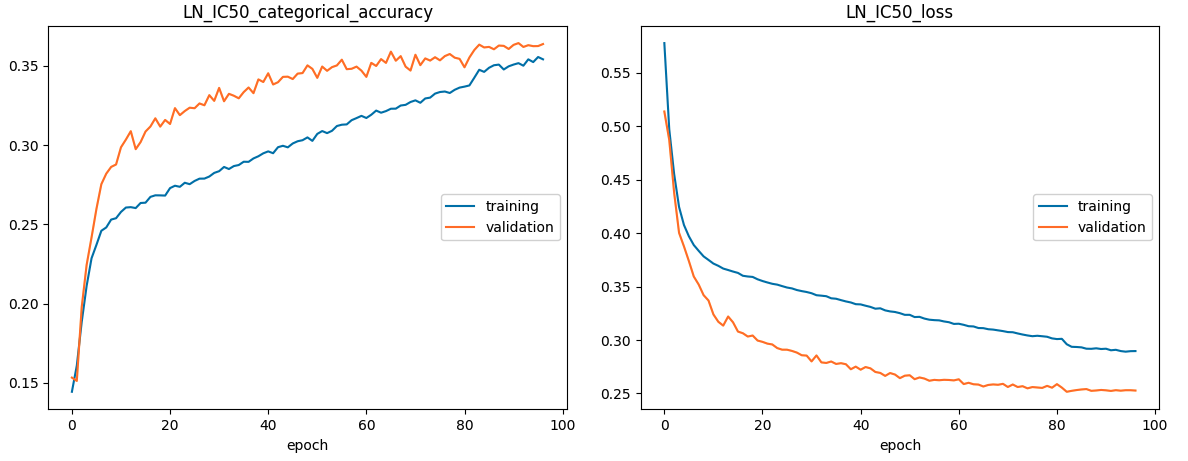
\includegraphics[width=1\textwidth]{figures/neural_net_classification/classification_mse_v2.png}
    \caption{Model training progress applying categorical focal loss.}
    \label{fig:train_class_net_v2}
\end{figure}

\begin{table}[H]
    \centering
    \begin{tabular}{|l|c|}
    \hline
    \textbf{Validation Metric} & \textbf{Best Value} \\
    \hline
    LN\_IC50\_Categorical\_Accuracy & 0.383 \\
    LN\_IC50\_Loss & 0.504 \\
    \hline
    \end{tabular}
    \caption{Best validation results for LN\_IC50 metrics using focal loss.}
    \label{tab:best_val_ln_ic50_focal}
\end{table}

The results obtained after this new modification are extremely interesting. Both models, the previous one and this one, perform better on the validation set than on the training set. However, in this case, it can be seen that it was necessary to reduce the learning rate halfway through training in order to continue improving. In the previous case, the learning rate did not need to be reduced to obtain a substantial improvement in performance, as illustrated in Figure~\ref{fig:train_class_net_v1}. 

In this second training session, although better results are obtained than in the previous one, as shown in Table~\ref{tab:best_val_ln_ic50_focal}, the model's progression is less promising, as can be seen in igure~\ref{fig:train_class_net_v2}.

This can lead to two main ideas:

\begin{itemize}
    \item The dataset contains some unbalanced classes. Therefore, in order to learn how to classify them correctly, the first model must invest more time, while the second, thanks to the focal error function, is able to learn faster. However, this second model reaches a plateau even after reducing the learning rate.
    \item Although the model that uses categorical error learns more slowly, it seems to have more potential for improvement, since in the case of the model that incorporates focal loss, the performance slope is less pronounced.
\end{itemize}

\subsubsection{Expansion paths: Priorities}

Due to the high number of outputs in the current architecture, the model may attempt to learn all targets with equal emphasis, or worse, prioritize outputs that are not related to \(LN\_IC_{50}\). To address this, a weighting strategy was proposed in which the importance of each output is adjusted. This aims to improve the prediction performance for \(LN\_IC_{50}\) by giving it higher priority during training.

This modification was implemented using the Keras Functional API, as shown in Listing~\ref{cod:class_net_v3}. The loss contributions from all output layers were maintained, except for the one corresponding to \(LN\_IC_{50}\), which was assigned 50\% more weight. The objective is to ensure that the model continues to consider the auxiliary outputs while explicitly encouraging better performance on the primary target, \(LN\_IC_{50}\).

Thanks to this approach, a considerable improvement was achieved during training, as shown in Figure~\ref{fig:train_class_net_v3} and Table~\ref{tab:best_val_ln_ic50_wheighting}. Here, both accuracy and error have improved. Once again, it was necessary to reduce the learning rate during training.

\begin{figure}[H]
    \centering
    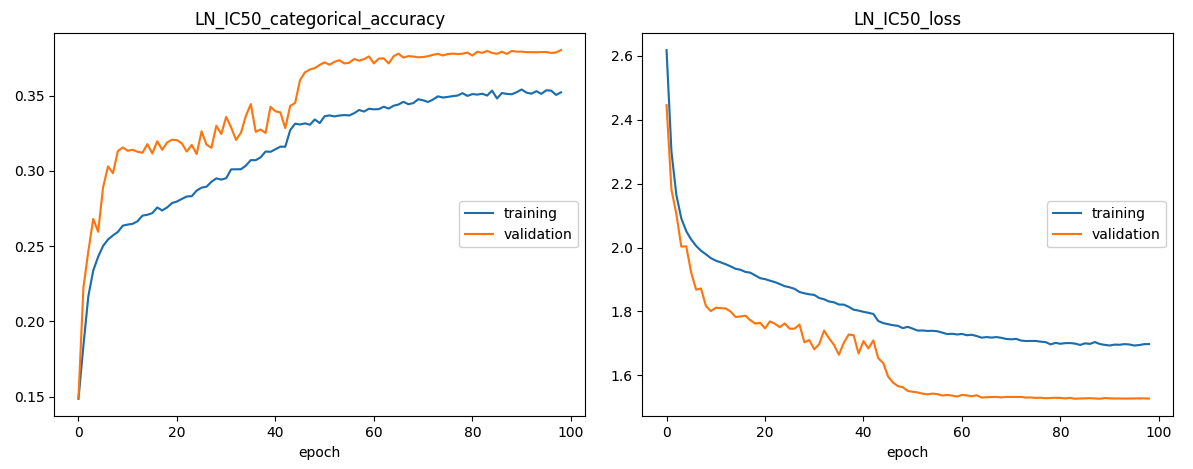
\includegraphics[width=1\textwidth]{figures/neural_net_classification/classification_mse_v3.png}
    \caption{Model training progress by changing the importance of outputs.}
    \label{fig:train_class_net_v3}
\end{figure}

\begin{table}[H]
    \centering
    \begin{tabular}{|l|c|}
    \hline
    \textbf{Validation Metric} & \textbf{Best Value} \\
    \hline
    LN\_IC50\_Categorical\_Accuracy & 0.384 \\
    LN\_IC50\_Loss & 2.496 \\
    \hline
    \end{tabular}
    \caption{Best validation results for \(LN\_IC_{50}\) metrics after applying output weighting.}
    \label{tab:best_val_ln_ic50_wheighting}
\end{table}

Everything seems to indicate that adjusting the weights of the outputs provides an increase in the model's performance. Likewise, during this training, it can be observed how, once again, the categorical cross-entropy error function has provided the necessary dynamism to improve the quality of the predictions by reducing the learning rate in around the epoch 80.

\subsubsection{Refinement of the loss function}

The experimental results suggest that performance can be improved by carefully designing the training process, specifically through a combination of output weighting and an appropriately chosen loss function.

While selecting the optimal combination of weights often involves empirical tuning, the choice of loss function is more critical, as it must be tailored to both the characteristics of the data and the nature of the problem. It is important to recall that the objective is not merely to predict the exact number of doses, but to minimize the severity of misclassifications. For example, mispredicting by one dose is less significant than mispredicting by five. Consequently, the loss function must reflect this asymmetry in error severity.

Additionally, the loss must support effective learning; otherwise, there is a risk of stagnation during training. To address these requirements, a custom loss function was developed for the final version of the classification model, as shown in Listing~\ref{cod:class_net_v4}. This function penalizes predictions progressively based on their distance from the correct class, encouraging the model to make closer, even if not exact, predictions. As a result, the number of highly incorrect classifications is significantly reduced.

As a result of all these modifications, the model significantly increases performance and reduces the difference between training and validation, all of which can be seen in Figure~\ref{fig:train_class_net_v4}. This translates into more accurate and reliable predictions outside the training set.

\begin{figure}[H]
    \centering
    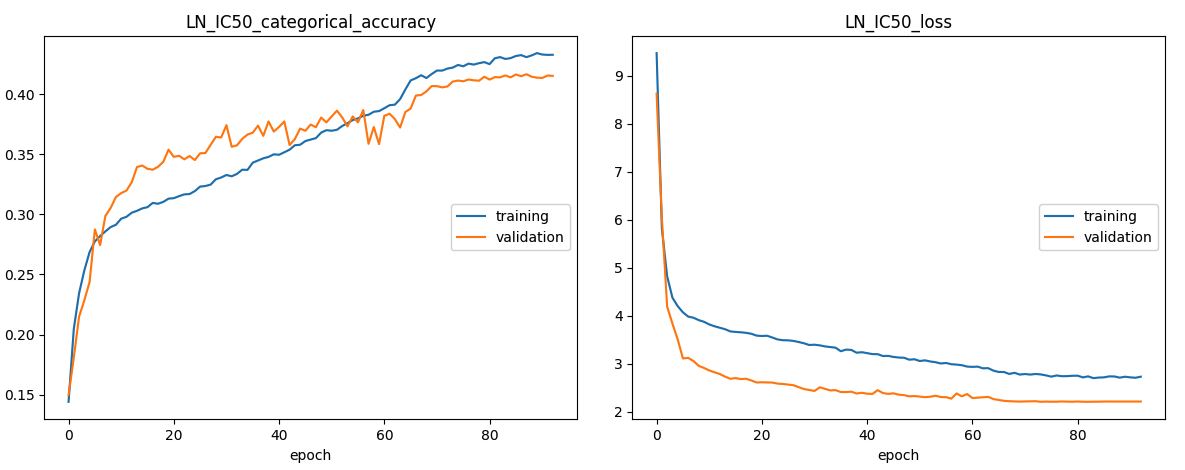
\includegraphics[width=1\textwidth]{figures/neural_net_classification/classification_custom_loss.png}
    \caption{Progress of model training applying a customised error function, which takes into account both accuracy and the difference between the actual and predicted values.}
    \label{fig:train_class_net_v4}
\end{figure}

\begin{table}[H]
    \centering
    \begin{tabular}{|l|c|}
    \hline
    \textbf{Validation Metric} & \textbf{Best Value} \\
    \hline
    LN\_IC50\_Categorical\_Accuracy & 0.412 \\
    LN\_IC50\_Loss & 2.195 \\
    \hline
    \end{tabular}
    \caption{Best validation results for LN\_IC50 metrics using the custom loss function.}
    \label{tab:best_val_ln_ic50_customloss}
\end{table}

\begin{figure}[H]
    \centering
    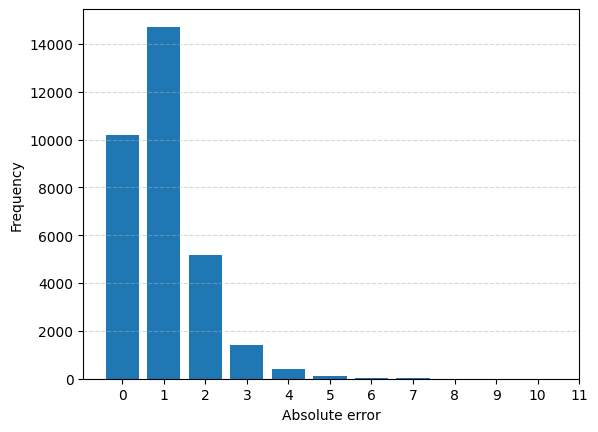
\includegraphics[width=1\textwidth]{figures/neural_net_classification/catogorical_net_barplot.png}
    \caption{Bar chart representation of the absolute error committed in the test set. It allows us to verify that the model predicts with a low degree of error.}
    \label{fig:train_class_net_v4_barplot}
\end{figure}

\begin{table}[H]
    \centering
    \begin{tabular}{|l|c|}
    \hline
    \textbf{Test Metric} & \textbf{Value} \\
    \hline
    MSE & 1.218 \\
    RMSE & 1.103 \\
    R\textsuperscript{2} & 0.878 \\
    \hline
    \end{tabular}
    \caption{Regression performance metrics on the test set for LN\_IC\_50 using a neural network with custom loss function.}
    \label{tab:test_regression_metrics:net_class_v4}
\end{table}

However, there is one aspect that cannot be assessed from the graph in Figure~\ref{fig:train_class_net_v4}. In this iteration, an error function has been defined that should prevent large discrepancies between reality and prediction. This feature is corroborated in Figure~\ref{fig:train_class_net_v4_barplot}, which illustrates a histogram in which the highest percentage of errors are between 0 and 1 doses. Therefore, the model effectively meets expectations.

Reaching this point in the research represents a milestone in the study, as the model is capable of deciding how many doses to administer, with a single-dose error in most cases. This allows for better management of prescriptions, thus improving patients' quality of life.

\section{Testing XGBoost as a classifier}

In this section, the method applied is XGBoost in a multi-class classification setting, using the discretised variable \(LN\_IC_{50}\) as in previous experiments. The aim is to evaluate its predictive power and compare it with the results obtained using deep learning approaches.

Beyond accuracy, it is particularly interesting how XGBoost handles the ordinal nature of the target variable, where misclassifying a class by 1 is much less serious than misclassifying it by 5 or more. To achieve this, evaluations will be carried out using standard metrics, such as accuracy, but also some that take into account the distance between the prediction and the actual classes, including MAE and RMSE.

As the dynamic applied throughout the research, the model will be refined as the reading progresses. First, training will be carried out where only accuracy will be taken into account, and then training will also evaluate the difference between prediction and expected class. This initial process will allow us to compare and verify that this approach is the most appropriate.

\subsubsection{Focusing on classification}

To conduct the research using xgboost and focusing solely on the accuracy of the result, the most appropriate objective function is softmax. This setting enable multi-class classification, by directly modeling the probability distribution over all classes. Otherwise, the architecture would have to be modelled as one vs rest system, which would require a binary classifier for each class. This would increase the time and effort required.

For evaluating model performance, the chosen loss function is categorical cross-entropy, referred to in the XGBoost Python library as Multi-Class Log Loss (mlogloss). This metric is particularly appropriate because it not only assesses classification correctness but also takes into account the confidence of the predicted probabilities, in this way, a more nuanced assessment is provided than simple accuracy.

The flaw in this approach is that it does not take into account the severity of major errors. In fact, Figure~\ref{fig:barplot_xgboost_v1} shows how the results obtained using this model falls significantly short of those produced by the neural network. This is further supported by the metrics shown in Table~\ref{tab:xgboost_classification_metrics_v1}, which reveal a substantial increase in error.

\begin{figure}[H]
    \centering
    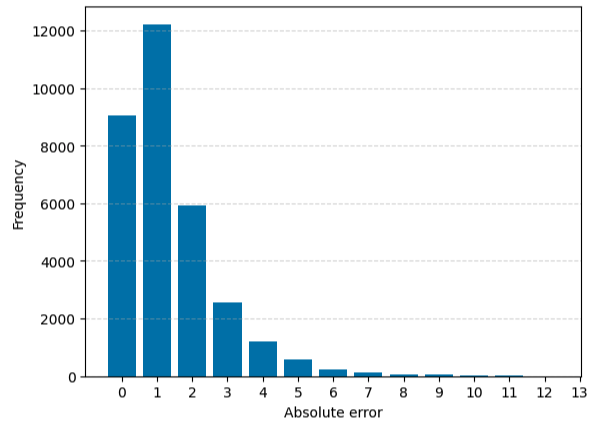
\includegraphics[width=1\textwidth]{figures/xgboost_class/xgboost_class_v1_softmax.png}
    \caption{Representation of the absolute error committed with the test set using XGBoost and softmax. A substantial increase in error is observed, with the largest error committed being 11.}
    \label{fig:barplot_xgboost_v1}
\end{figure}

\begin{table}[H]
    \centering
    \begin{tabular}{|l|c|}
    \hline
    \textbf{Test Metric} & \textbf{Value} \\
    \hline
    MSE & 2.766 \\
    RMSE & 1.663 \\
    R\textsuperscript{2} & 0.724 \\
    \hline
    \end{tabular}
    \caption{Performance metrics on the test set for \(LN\_IC_{50}\) using XGBoost classifier predictions interpreted as numerical outputs.}
    \label{tab:xgboost_classification_metrics_v1}
\end{table}

\subsubsection{Prioritizing distance to the right class}

Applying a function that shows the importance of being close to the correct class should improve the quality of the model. In the case of XGBoost, the function used is the mean square error (MSE). In addition, it is necessary to modify the evaluation metric, in this case the root mean square error (RMSE), to facilitate the interpretation of progress.

After a series of training sessions, a result similar to that of neural networks was obtained, without reaching the same quality, but improving on the previous version. This can be seen in Figure~\ref{fig:barplot_xgboost_v2}, which shows how the proportion changes, increasing the number of cases in which only one error is made, or even none at all. It also reduces all the others, as reflected in the metrics in Table~\ref{tab:xgboost_classification_metrics_v2}, where the maximun error is 12.

\begin{figure}[H]
    \centering
    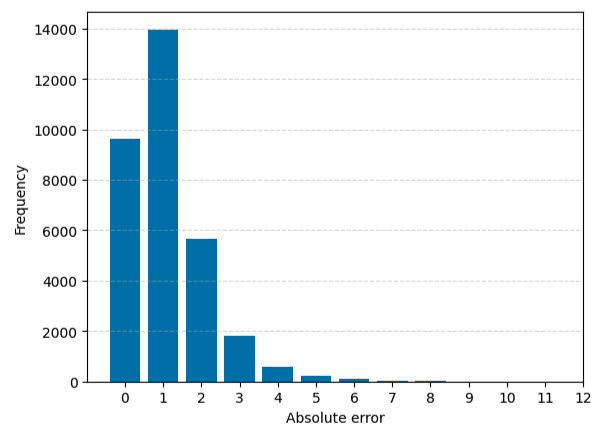
\includegraphics[width=1\textwidth]{figures/xgboost_class/xgboost_class_v2_mse.png}
    \caption{Representation of the absolute error committed with the test set using XGboost and MSE. A substantial increase in error is observed, with the largest error committed being 12.}
    \label{fig:barplot_xgboost_v2}
\end{figure}

\begin{table}[H]
    \centering
    \begin{tabular}{|l|c|}
    \hline
    \textbf{Test Metric} & \textbf{Value} \\
    \hline
    MSE & 2.381 \\
    RMSE & 1.543 \\
    R\textsuperscript{2} & 0.834 \\
    \hline
    \end{tabular}
    \caption{Performance metrics on the test set using XGBoost with \texttt{reg:squarederror}.}
    \label{tab:xgboost_classification_metrics_v2}
\end{table}

By applying the same distance-aware approach used in neural networks to the XGBoost model, the result obtained is very similar. Two key aspects of this result must be taken into account:

\begin{itemize}
    \item Accuracy of predictions: While the overall performance is similar in terms of trend, the quality of the model is slightly lower. the model exhibits a higher number of instances where the error is greater than 3, a threshold that should not be exceeded too often, as such deviations could negatively impact clinical outcomes.
    \item Training time and cost: One of the major advantages of using XGBoost lies in its training efficiency. The model can be trained significantly faster and with much lower computational overhead compared to neural networks, which often require extensive resources and time to achieve optimal performance.
\end{itemize}


\section{SHAP: The reasons must be known.}

This chapter focuses on applying all the knowledge acquired during the research to understand what the best trained models have learned. The objective is to extract the linear or non-linear relationships that the model has learned from the data.

This approach allows, on the one hand, to validate the correct learning of the model. For example, it could be the case that to infer the response, the model looks at patterns that have nothing to do with the efficiency of a drug, as would be the case with a model that groups several cases because it identifies that they have the same doctor. This knowledge, although entirely valid, implies that the learning has not acquired the quality it should, as it should predict based on a patient's data, not on who is treating them. On the other hand, knowing the features on which a model is based and to what extent can represent a major advance in cancer research, open up new avenues of research or demonstrate previously unknown theories.

Throughout this research, regressors based on two different modeling approaches were trained. First, models based on neural networks were trained, which are particularly capable of finding non-linear and complex relationships. Then, research was conducted on the feasibility of using tree-based models, hough generally less performant than neural networks, offer faster training times and lower computational cost. Thus, there are models based in two different type of algorithm, a network-based model and a tree-based model. Among them, the model that provides the best results should be selected, as it is the one that generalises best. Thus, given that the best network-based model, whose metrics are shown in Table~\ref{tab:metrics_multiplicative_gating}, offers much better performance than the tree-based model, whose metrics are shown in Table~\ref{tab:model_performance_xgboost}, the network-based architecture should be used.

To understand the reasons behind the neural network's predictions, the technique used in this study was SHAP, as it allows explainability to be applied not only locally but also globally.

In Figure~\ref{fig:shap_values}, the SHAP values of a set of 200 examples are shown. This representation provides a very intuitive visualisation of what is happening within the model, slightly dispelling that black box perception.

\begin{figure}[H]
    \centering
    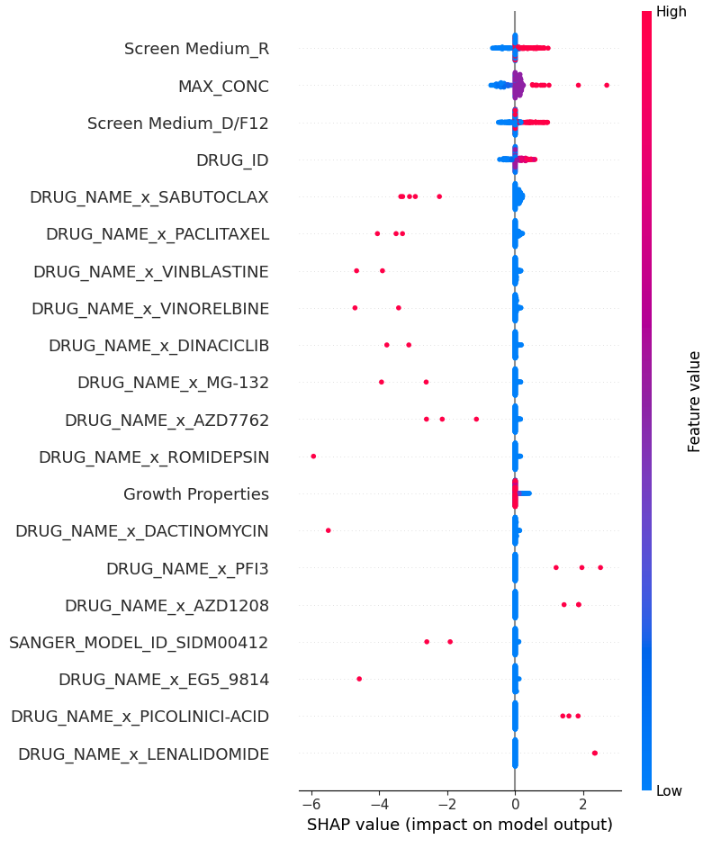
\includegraphics[width=1\textwidth]{figures/shap/shap_values.png}
    \caption{Shap summary plot with 200 examples. This one shows how the model behaves based on the values of its most representative variables.}
    \label{fig:shap_values}
\end{figure}

To interpret the image, it is important to note that all variables beginning with "DRUG\_NAME", "Screen Medium", or "SANER" have been one-hot encoded. This encoding explains the pattern of numerous blue dots and only a few red ones, indicating that the model primarily values the absence of these features. In contrast, the variable "DRUG\_ID" retains its original numerical values. Thus, the blue dots corresponding to these variables indicate that they are not present in the instance. For example, in the case of drug names, the blue dots represent those cases in which the drug in question has not been administered.

Figure~\ref{fig:shap_values} suggests that when the network detects that drugs such as Sabutoclax, Paclitaxel Vinblastine are recessed, the probability of predicting a low value for the \(LN\_IC_{50}\) variable increases, since all of them contribute to reducing the prediction value. Applying this knowledge to real life could mean that these drugs are more aggressive against cancer and therefore the amount needed is lower. In fact, according to several studies \cite{Hu2018Sabutoclax, DAguanno2020Bcl2}, Sabutoclax is mainly used in cases where the patient experiences some resistance to standard therapies.

Similarly, it can be seen that when the maximum concentration increases the model, so does the probability of predicting a high value for \(LN\_IC_{50}\).

Regarding the listed drugs, the presence of the first 9 appears to be associated with lower predictions for the \(LN\_IC_{50}\) variable, which is considered a favorable outcome for patients. Notably, one of the 20 most influential features is linked to the blood sample type. Its presence consistently contributes to lower \(LN\_IC_{50}\) values, reinforcing the hypothesis that genetic or biological factors, such as the type of sample, may significantly influence a patient's response to cancer treatments. This finding supports the broader theory that the human genome plays a crucial role in drug sensitivity.

The dependency plot for the variable SANGER\_MODEL\_ID\_SIDM00412, illustrated in Figure~\ref{fig:dependenceSanger}, reveals that, in the cases analysed by SHAP, when this specific blood sample is present, the value of the Growth Properties feature is never set to D/F12. This combination is associated with negative SHAP values for the target variable  \(LN\_IC_{50}\), suggesting that patients corresponding to this sample tend to require a lower dosage of medication. This may indicate a favorable drug sensitivity profile for this particular biological condition.

\begin{figure}[H]
    \centering
    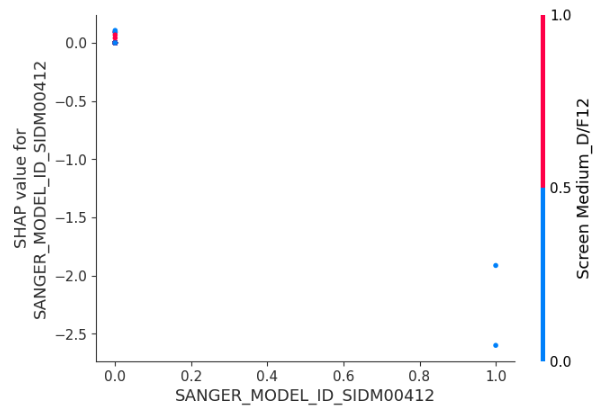
\includegraphics[width=1\textwidth]{figures/shap/dependence_plot_sanger.png}
    \caption{Dependence plot of variable SANGER\_MODEL\_ID\_SIDM00412 obtained using SHAP. Obtained by analysing 200 examples.}
    \label{fig:dependenceSanger}
\end{figure}
    \chapter{Conclusions}\label{cap:conclusiones}

This thesis has explored the intersection between machine learning and precision oncology, with the aim of predicting drug sensitivity in cancer using genomic data. Leveraging the Genomics of Drug Sensitivity in Cancer (GDSC) dataset, the study developed and evaluated several predictive models focused primarily on estimating the value \( \text{LN\_IC}_{50} \), a key indicator of drug efficacy.

The initial phase of the research focused on regression, where neural networks demonstrated a strong ability to model complex, non-linear relationships inherent in genomic data. Through careful preprocessing, dimensionality reduction, and hyperparameter optimisation, the best regressor achieved an RMSE of less than 0.5, demonstrating the feasibility of accurately estimating drug response.

To more closely approximate real clinical decisions, the problem was subsequently discretised, transforming it into a classification task to emulate dose estimation. Several approaches were tested, including categorical cross-entropy, focal loss, and custom-designed loss functions that penalised large prediction errors more severely. Despite the inherent complexity and class imbalance, the network maintained reasonable accuracy while respecting the ordinal nature of the problem.

In addition, explainability techniques such as SHAP were explored to interpret model decisions. These insights revealed the most influential genomic and pharmacological characteristics, supporting the hypothesis that patient-specific genomic profiles significantly influence drug efficacy. This not only improved the transparency of the model but also suggested potential biological insights that warrant further investigation.

Comparative experiments with tree-based models, such as XGBoost, confirmed that, although they offer faster training and lower resource consumption, they tend to underperform deep learning models when capturing complex data relationships.

Finally, the work highlights the importance of personalised medicine and the role that machine learning can play in improving treatment strategies. The results demonstrate that integrating genomic data with predictive models offers a promising avenue towards more effective and individualised cancer therapies.
    
    \appendix
\addcontentsline{toc}{chapter}{Appendix}
\chapter*{Appendix}

\vspace{10pt}
\lstinputlisting[
    language=Python,
    label=cod:obsoletes,
    caption={Find obsolete variables and determine the size of each variable's domain.}
]{code/datat_representation/obsoletes.py}
\vspace{10pt}

\vspace{10pt}
\lstinputlisting[
    language=Python,
    label=cod:inconsistencesNameId,
    caption={Check for matching values between the drug ID and drug name variables.}
]{code/datat_representation/inconsistences_name_id.py}
\vspace{10pt}

\vspace{10pt}
\lstinputlisting[
    language=Python,
    label=cod:gaussTest,
    caption={Checking whether \(LN\_IC_{50}\) follows a normal distribution.}
]{code/datat_representation/normal_distribution_test.py}
\vspace{10pt}

\vspace{10pt}
\lstinputlisting[
    language=Python,
    label=cod:supplierConsistence,
    caption={Code intended to check the different suppliers assigned to each drug name.}
]{code/datat_representation/supplier_name_consistence.py}
\vspace{10pt}

\vspace{10pt}
\lstinputlisting[
    language=Python,
    label=cod:columnTransformer,
    caption={Application of ColumnTransformer to map the data.}
]{code/datat_representation/column_transformer.py}
\vspace{10pt}

\vspace{10pt}
\lstinputlisting[
    language=Python,
    label=cod:ordinalEncoder,
    caption={Encoding data in numerical format using Ordinal Encoder.}
]{code/datat_representation/ordinal_encoder.py}
\vspace{10pt}

\vspace{10pt}
\lstinputlisting[
    language=Python,
    label=cod:knnImputer,
    caption={Imputation of values using KnnImputer.}
]{code/datat_representation/knn_imputer.py}
\vspace{10pt}

\vspace{10pt}
\lstinputlisting[
    language=Python,
    label=cod:pythonGenerateNet,
    caption={Function to generate a neural network. This code generates a very simple dense network, but we only want it to know which loss function to choose.}
]{code/loss_checker/generate_model.py}
\vspace{10pt}

\lstinputlisting[
    language=Python,
    label=cod:pythonCompileNet,
    caption={Function to compile, show the losses during learning, do a evaluation with test set and return the model trained.}
]{code/loss_checker/train_model.py}
\vspace{10pt}

\lstinputlisting[
    language=Python,
    label=cod:pythonShowMetrics,
    caption={Functions to show some metrics about the model. Also, we display a plot where you can see how much near is the predicted values from the real ones.}
]{code/loss_checker/evaluate.py}
\vspace{10pt}

\vspace{10pt}
\lstinputlisting[
    language=Python,
    label=cod:reg_addition_desbalanced,
    caption={Definition of Soft-ordering with 1D convolutional architecture using tensorflow.}
]{code/neural_nets/reg_addition_desbalanced.py}
\vspace{10pt}


\vspace{10pt}
\lstinputlisting[
    language=Python,
    label=cod:reg_addition_balanced,
    caption={Definition of Soft-ordering with 1D convolutional architecture using SiLU as activation function.}
]{code/neural_nets/reg_addition_balanced.py}
\vspace{10pt}

\vspace{10pt}
\lstinputlisting[
    language=Python,
    label=cod:intervalEntropy,
    caption={Representation of entropy evolution based on the number of bins.}
]{code/datat_representation/intervals_entropy.py}
\vspace{10pt}

\vspace{10pt}
\lstinputlisting[
    language=Python,
    label=cod:tsne,
    caption={Calculation of dimensionality reduction using t-SNE for data representation while respecting local distances.}
]{code/datat_representation/tsne.py}
\vspace{10pt}

\vspace{10pt}
\lstinputlisting[
    language=Python,
    label=cod:umap,
    caption={Calculation of dimensionality reduction using UMAP for data representation while respecting global and local distances.}
]{code/datat_representation/umap.py}
\vspace{10pt}

\vspace{10pt}
\lstinputlisting[
    language=Python,
    label=cod:class_net_v1,
    caption={First adaptation of the regressor network in the process of obtaining a classifier.}
]{code/neural_nets/classification_net_v1.py}
\vspace{10pt}

\vspace{10pt}
\lstinputlisting[
    language=Python,
    label=cod:class_net_v2,
    caption={Testing a different function to check for changes in model performance.}
]{code/neural_nets/classification_net_v2.py}
\vspace{10pt}

\vspace{10pt}
\lstinputlisting[
    language=Python,
    label=cod:class_net_v3,
    caption={Assigning importance to target variables for the purpose of obtaining better results in \(LN\_IC_{50}\).}
]{code/neural_nets/classification_net_v3.py}
\vspace{10pt}

\vspace{10pt}
\lstinputlisting[
    language=Python,
    label=cod:class_net_v4,
    caption={Definition of a custom error function, including categorical cross entropy and MSE.}
]{code/neural_nets/classification_net_v4.py}
\vspace{10pt}
    % Bibliografía
    \bibliographystyle{unsrtnat}
    \bibliography{bibliografia.bib}
        

% Fin del documento
\end{document}
